\documentclass[aps,preprint,tightenlines,floatfix,superscriptaddress,nofootinbib,showpacs]{revtex4-1}
\pdfoutput=1
\usepackage{graphicx}
%\usepackage{dcolumn}
\usepackage{amsfonts}
\usepackage{hhline}
\usepackage{multirow}
\usepackage{array}
%\usepackage{longtable}
\usepackage{amsmath}
\usepackage{amssymb}
\usepackage{maybemath}
%\usepackage[italic]{hepparticles}
\usepackage{float}
\usepackage[lofdepth,lotdepth]{subfig}
\usepackage[countmax]{subfloat}
\usepackage{cancel}
%\usepackage[nodisplayskipstretch]{setspace}
%\setstretch{1.5}
%\usepackage{caption}
%\usepackage{subcaption}
\setlength{\oddsidemargin}{-1in}
\addtolength{\oddsidemargin}{24mm} \setlength{\textwidth}{170mm}
\setlength{\topmargin}{-0.55in} \setlength{\headheight}{10mm}
\setlength{\headsep}{0mm} \setlength{\textheight}{230mm}
\def\beq{\begin{equation}}
\def\eeq{\end{equation}}
\def\bea{\begin{eqnarray}}
\def\eea{\end{eqnarray}}
\def\nn{\nonumber}
\def\sss{\scriptstyle}
\def\lft{{\scriptstyle L}}
\def\rht{{\scriptstyle R}}
\def\roughly#1{\mathrel{\raise.3ex\hbox
{$#1$\kern-.75em\lower1ex\hbox{$\sim$}}}}
\def\lsim{\roughly<}
\def\gsim{\roughly>}
\def\tbslash{\tbar\hspace{-10pt}\not{}\hspace{4pt}}
\def\tslash{t\hspace{-10pt}\not{}\hspace{4pt}}
\def\lpslash{l^+\hspace{-10pt}\not{}\hspace{4pt}}
\def\lmslash{l^-\hspace{-10pt}\not{}\hspace{4pt}}
\def\nslash{n\hspace{-10pt}\not{}\hspace{4pt}}
\def\ntbslash{n_{\tbar}\hspace{-10pt}\not{}\hspace{4pt}}
%%%%%%%%%%%%%%%%%%%%%%%%%%%%%%%%%%%%%%%%%%%%%%%%%%%%%%%%%%%%%%%%%%%%%%%%%%%%%%%
\newcommand{\note}[1]{\marginpar{{\small\begin{center}{\it #1}\end{center}}}}
%%%%%%%%%%%%%%%%%%%%%%%%%%%%%%%%%%%%%%%%%%%%%%%%%%%%%%%%%%%%%%%%%%%%%%%%%%%%%%%
\def\tbar{\bar{t}}
%\def\tbar{{\overline{t}}}
\def\bbar{\bar{b}}
\def\qbar{\bar{q}}
\def\nubar{{\bar{\nu}}_{\ell}}
\def\tbbc{t \to b \bbar c}
\def\tauprocess{\tau\rightarrow K\pi\pi\nu_{\tau}}
\def\ppprocess{pp\to t\,\left(\rightarrow b {\ell}^+ \nu_{\ell}\right) \tbar\,\left(\rightarrow\bbar {\ell}^-\nubar\right)\,H}
\def\bppprocess{{\boldmath $pp\to t \tbar H\to \left(b {\ell}^+ \nu_{\ell}\right)\left(\bbar {\ell}^-\nubar\right)H$}}
\def\ggprocess{gg\to t \tbar H\to\left(b l^+ \nu_l\right)\left(\bbar l^-\nubar\right)H}
\def\qqprocess{q\qbar\to t \tbar H\to\left(b l^+ \nu_l\right)\left(\bbar l^-\nubar\right)H}
\def\kp{\kappa_t}
\def\kpt{\tilde{\kappa}_t}
\def\MG{\mbox{MadGraph 5}}
\def\tm#1{\texttt{TM-{#1}}}
\def\ex#1{\texttt{EX-{#1}}}
\def\Ahat{\hat A_i^{\sigma}}
\def\madg{MadGraph~5}
\def\TPa{\epsilon(t,\tbar,n_t,n_{\tbar})}
\def\TPb{\epsilon(Q,\tbar,n_t,n_{\tbar})}
\def\TPc{\epsilon(Q,t,n_t,n_{\tbar})}
%%%%%%%%%%%%%%%%%%%%%%%%%%%%%%%%%%%%%%%%%%%%%%%%%%%%%%%%%%%%%%%%%%%%%%%%
%%%%%
%for editing purposes
\usepackage[normalem]{ulem}
\usepackage{color}
\definecolor{BrickRed}{cmyk}{0,0.89,0.94,0.28}
\definecolor{DarkGreen}{cmyk}{1,0,1,0.5}
\definecolor{Blue}{cmyk}{1,1,0,0}
\definecolor{BurntOrange}{cmyk}{0,0.51,1,0}

\def\hldl#1{\textcolor{BrickRed}{\textsf{#1}}}
\def\hlps#1{\textcolor{DarkGreen}{\textsf{#1}}}
\def\hlkk#1{\textcolor{Blue}{\textsf{#1}}}
\def\hlas#1{\textcolor{BurntOrange}{\textsf{#1}}}
\def\soutdl{\bgroup\markoverwith{\textcolor{BrickRed}{\rule[0.5ex]{2pt}{0.4pt}}}\ULon}
\def\soutps{\bgroup\markoverwith{\textcolor{DarkGreen}{\rule[0.5ex]{2pt}{0.4pt}}}\ULon}
\def\soutkk{\bgroup\markoverwith{\textcolor{Blue}{\rule[0.5ex]{2pt}{0.4pt}}}\ULon}
\def\soutas{\bgroup\markoverwith{\textcolor{BurntOrange}{\rule[0.5ex]{2pt}{0.4pt}}}\ULon}

\def\mhldl#1{\textcolor{BrickRed}{\ensuremath{#1}}}
\def\mhlps#1{\textcolor{DarkGreen}{\ensuremath{#1}}}
\def\mhlkk#1{\textcolor{Blue}{\ensuremath{#1}}}
\def\mhlas#1{\textcolor{BurntOrange}{\ensuremath{#1}}}
\def\msoutdl#1{\text{\soutps{\ensuremath{#1}}}}
\def\msoutps#1{\text{\soutps{\ensuremath{#1}}}}
\def\msoutkk#1{\text{\soutps{\ensuremath{#1}}}}
\def\msoutas#1{\text{\soutps{\ensuremath{#1}}}}
%%%%%%%%%%%%%%%%%%%%%%%%%%%%%%%%%%%%%%%%%%%%%%%%%%%%%%%%%%%%%%%%%%%%%%%%
\begin{document}
\vspace*{2cm}

\title{{\boldmath Pseudoscalar top-Higgs coupling:  Exploration of $\mathrm{CP}$-odd observables to 
resolve the sign ambiguity
}}

\def\tayloru{\affiliation{\it Physics and Engineering Department,
    Taylor University, \\ 236 West Reade Ave., Upland, IN 46989, USA \vspace*{1mm}}}

%\def\tayloru{\affiliation{\it Physics and Engineering Department,
%    Taylor University, \\ 236 West Reade Ave., Upland, IN 46989, USA \vspace*{8mm}}}

\def\laplata{\affiliation{\it IFLP, CONICET -- Dpto. de F\'{\i}sica,
    Universidad Nacional de La Plata, C.C. 67, 1900 La Plata,
    Argentina \vspace*{8mm}}}

\author{Nicolas Mileo}
\email{mileo@fisica.unlp.edu.ar}
\laplata

\author{Ken Kiers}
\email{knkiers@taylor.edu}
\tayloru

\author{Alejandro Szynkman}
\email{szynkman@fisica.unlp.edu.ar}
\laplata

\author{Daniel Crane \vspace*{4mm}}
\email{dkcrane@mtu.edu}
\tayloru

\author{Ethan Gegner}
\email{ethan\_gegner@taylor.edu}
\tayloru

\date{\vspace*{2mm}\today \\\bigskip\bigskip}

\begin{abstract}
\vspace*{4mm} We present a collection of $\mathrm{CP}$-odd observables
for the process $\ppprocess$ that are linearly dependent on the scalar
($\kp$) and pseudoscalar ($\kpt$) top-Higgs coupling and hence
sensitive to the corresponding relative sign. The proposed observables
are based on triple product (TP) structures that we extract
from the expression of the differential cross section in terms of the
spin vectors of the top and antitop quarks. In order to explore other
possibilities, we progressively modify these TPs, first
by combining them, and then by replacing the spin vectors by the
lepton momenta or the $t$ and $\tbar$ momenta by their visible parts.
Assuming an integrated luminosity that is consistent with that
  envisioned for the HL-LHC, we find that the most
promising observable can disentangle the hypotheses $\kp=1,\kpt=\pm 1$
by more than the $\sim 20\sigma$ statistical level.  In
the case of observables that do not need the reconstruction of the $t$
and $\tbar$ momenta, the power of discrimination is up to the $\sim
16\sigma$ statistical level for the same number of events. We also show that the
capability of the most promising observables for separating the
$\mathrm{CP}$-mixed hypotheses preveals even when a number of events
plausible within the short term LHC is considered. 

%We also show that the sensitivity of the most promising observables is not spoiled when a number of events affordable by the short term LHC is considered.

%We also show that even when the number of events is reduced by an order of magnitude the most promising observables are still useful for testing the couplings
\end{abstract}
\maketitle
%%%%%%%%%%%%%%%%%%%%%%%%%%%%%%%%%%%%%%%%%%%%%%%%%
\section{Introduction}
\label{sec1}
After the discovery of a new boson $H$ by the ATLAS \cite{atlasH} and
CMS \cite{cmsH} collaborations, it has become of crucial importance
 to determine its physical
 properties with the highest possible precision.
 The study of the new boson's couplings
 to fermions is of great relevance
 and will allow us to better understand this particle's $\mathrm{CP}$-transformation
   properties, as well as the
extent to which this particle is consistent with the Higgs boson
predicted by the Standard Model (SM) of particle physics.
It is of particular importance to test the coupling of the putative 
Higgs boson to
the top quark.  This coupling governs
the main Higgs boson production mechanism (which proceeds via gluon fusion)
and it contributes to the
important Higgs boson decay mode to two photons.
It is also
involved in the scalar-field naturalness problem -- giving rise to the
leading dependence on the cut-off energy scale in the corrections to
the Higgs mass -- and it may play an important role in the mechanism for electroweak symmetry breaking.\par

Given that the main Higgs boson production
process is dominated by a top quark loop and that
the diphoton and digluon decay channels are also mediated by a top
loop, these processes provide constraints on the scalar and
pseudoscalar $tH$ couplings, $\kp$ and $\kpt$
\cite{constraints1,constraints2, constraints3,constraints4}.
     However,
these constraints assume that there are no other sources contributing
to the corresponding effective couplings; furthermore, in the case of the
diphoton decay channel (which also involves a $W$ boson loop), it is also
assumed that the
coupling of the Higgs boson to the $W$ is standard. In this sense, the
constraints derived from measurements of Higgs boson production and decay rates
 are indirect constraints. Electric dipole moments can also
impose stringent indirect constraints on $\kpt$ by assuming that there
are no new physics (NP) particles contributing to the loops of the
relevant diagrams and in the case of the EDM of the electron that the 
electron-Higgs coupling is that
predicted by the SM \cite{constraints1,edm}. In order to probe
the $tH$ coupling directly, processes with smaller cross sections need
to be taken into account.  \par

In contrast to the $\tau H$ coupling, which can be studied through the
decay $H\rightarrow \tau^+\tau^-$ \cite{tau},
the $tH$ coupling can only be tested directly via production processes, since the
Higgs boson is kinematically forbidden from decaying to a $t\tbar$ pair.
Two types of processes are of particular interest in this regard -- the
production of a Higgs boson in association with a $t\tbar$ pair
and in association with a single top or antitop. The cross section
for associated Higgs production with a single top (antitop)
is smaller than that for production with a $t\tbar$ pair, and involves
the interference between a diagram in which the Higgs is radiated from
the top (antitop) leg and one with the Higgs emitted from the
intermediate virtual $W$ boson. Interestingly, this implies that the contraints
on $\kp$ and $\kpt$ derived from $tH$ and $\tbar H$ production are
dependent on the assumption made regarding the coupling of the Higgs boson to the
$W$ gauge boson, $\kappa_W$. Nevertheless, it is important to note that the
interference between the above mentioned diagrams
can be exploited to determine the
relative sign between $\kp$ and $\kappa_W$ (see for example
Ref.~\cite{tHmaltoni}).  Associated Higgs production with a
$t\tbar$ pair has been studied by several authors, and
various observables sensitive to the couplings $\kp$ and $\kpt$ have
been proposed. Examples of such observables (all of which are
$\mathrm{CP}$-even) are the cross section, 
invariant mass distributions, the transverse Higgs momentum
distribution and the azimuthal angular separation between the $t$ and $\tbar$,
to name a few \cite{Guadagnoli,*Boosted,*Li,*Golden,*Khatibi}. Also, an approach based on weighted
moments and optimal observables has been developed in Ref.~\cite
{Gunion1,*Gunion2,*Gunion3,*Gunion} to discriminate the hypothesis of
a $\mathrm{CP}$-even Higgs from that of a $\mathrm{CP}$-mixed state
within the context of an $e^+ e^-$ as well as a $pp$ collider.
 Now, $\mathrm{CP}$-even observables are not
sensitive to the relative sign between the scalar and pseudoscalar
couplings $\kp$ and $\kpt$. Such observables are quadratically
dependent on these couplings and thus only provide an indirect measure
of $\mathrm{CP}$ violation. In order to be sensitive to the relative
sign between $\kp$ and $\kpt$, $\mathrm{CP}$-odd observables must be
considered. \par

Since the top quark decays before it can hadronize, its spin
information is passed on to the angular distributions of its decay
products in such a way that these particles work as spin analyzers.
As is well known, in the case of semileptonic top decay,
the charged lepton is the most powerful in this regard.
It is also known that the top quark and antiquark spins
are highly correlated in $t\tbar$ production,
a feature that
is manifested in the double angular distributions of the decay
products of the $t$ and $\tbar$ systems \cite{Mahlon1,*Mahlon2,*Mahlon3,*atwood}.
%The spin correlations
%between the $t$ and $\tbar$ are
%dependent in turn on the $t\tbar$ production mechanism, and in
In the case of
$t\tbar H$ associated production, the $t\tbar$ spin correlations
are also sensitive to the manner in which
the top couples to the Higgs boson. 
In fact, observables that exploit
the differences in the $t\tbar$ spin configurations were used in
Ref.~\cite{Biswas} to improve the discrimination of the $t\tbar H$ signal
from the dominant irreducible background $t\tbar b\bbar$, which does not
involve the Higgs boson. 

In this paper, we define a set of observables that are linearly dependent on
$\kp$ and $\kpt$ and are thus sensitive to the relative sign of these
couplings. The proposed observables are based on a particular set of
triple product (TP) structures that we extract naturally from the
expression for the differential cross section for $\ppprocess$,
making use of the fact that the $t$ and $\tbar$ decay products
contain spin information and are sensitive to the
nature of the $tH$ coupling, as noted above.
By using spinor techniques we relate the top
and antitop spin vectors to final state particle
momenta and separate the production process from the decay. This
allows to identify straightforwardly the contributions linearly
sensitive to the couplings.
 Further, the TPs correlations in these
contributions incorporate the $t$ and $\tbar$ spin vectors. Starting
with these TPs, we not only recover the observables given in
\cite{Ellis,Guadagnoli} but also propose additional possibilities that
increase the sensitivity. In order to establish a hierarchy in the
sensitivity of the TPs under analysis we investigate three different
types of observables by using simulated events: asymmetries, mean
values and angular distributions. We note that TP correlations have
been used in \cite{Valencia1,*Valencia2} in the context of top-quark
production and decay and in \cite{Valencia3} in the framework of
anomalous color dipole operators.  \par

The remainder of this paper is organized as follows. In
Sec.~\ref{sec2} we study the theoretical framework for the process
$\ppprocess$ and derive a general expression for the differential
cross section from which a first set of TP correlations is
extracted. In Sec.~\ref{sec3} we probe the sensitivity of these TPs to
the $tH$ coupling by using various $\mathrm{CP}$-odd
observables. Subsequent sections are dedicated to explore another
possibilities of $\mathrm{CP}$-odd observables. In particular,
observables based on TPs that incorporate the Higgs momentum are
discussed in Sec.~\ref{sec4}, whereas observables obtained without
using the $t$ and $\tbar$ momenta are studied in
Sec.~\ref{sec5}. Finally, Sec.~\ref{sec6} is devoted to the discussion
on the experimental feasibility of the most promising observables
encountered here. The main conclusions are summarized in
Sec.~\ref{sec7}.

%%%%%%%%%%%%%%%%%%%%%%%%%%%%%%%%%%%%%%%%%%%%%%%%%
%\newpage
%%%%%%%%%%%%%%%% Quitarlo %%%%%%%%%%%%%%%%%%%%%%%
\setlength{\abovedisplayskip}{10.6pt}
\setlength{\belowdisplayskip}{10.6pt}
%%%%%%%%%%%%%%%%%%%%%%%%%%%%%%%%%%%%%%%%%%%%%%%%%
%\section{Process \MakeLowercase{{\boldmath $pp\to t \bar{t}$}}$H\to$\MakeLowercase{{\boldmath $\left(b l^+ \nu_l \right) \left(\bar{b} l^-\bar{\nu}_l\right)$}}$H$. Theoretical framework}
\section{Theoretical framework for \MakeLowercase{{\boldmath $pp\to t(\to b {\ell}^+ \nu_{\ell})\,\bar{t}(\to\bar{b} {\ell}^-\bar{\nu}_{\ell})$}}$\,H$}
\label{sec2}

%

At the LHC $t\bar{t}H$ production proceeds via $q\bar{q}$
annihilation and $gg$ fusion processes. The relevant leading-order Feynman
diagrams are displayed in Fig.~\ref{fig1}, where the first two
rows show the $q\bar{q}$ and $gg$ $s$-channel diagrams, and
the last one depicts the $gg$ $t$-channel diagrams.  Three more
$gg$-initiated diagrams are obtained by exchanging the gluon
lines in the third row.
We describe the $tH$ coupling with the effective Lagrangian
%
\beq
\label{eq1}
\mathcal{L}_{t\bar{t}H}=-\frac{m_t}{v}(\kp \tbar t+i\kpt \tbar
\gamma_5 t)H,
\eeq
%
where $v=246~\mathrm{GeV}$ is the SM Higgs vacuum
expectation value, and the coefficients $\kp$ and $\kpt$ parameterize 
the scalar and pseudoscalar interaction, respectively. The
SM case is obtained for $\kp=1$ and $\kpt=0$, while the values $\kp=0$
and $\kpt\neq 0$ parameterize a $\mathrm{CP}$-odd Higgs boson.

Before turning to a discussion of $\mathrm{CP}$-odd observables,
it is useful to consider a few theoretical aspects of
the process $\ppprocess$.
In the following subsections we derive a ``factorized''
expression for the gluon fusion contribution to this process
and then use this expression
to isolate various mathematical quantities
that will be useful as we construct $\mathrm{CP}$-odd observables.\par

%%%%%%%%%%%%%%%%%%%% Figura 1%%%%%%%%%%%%%%%%%%%%%%%%%%%%%
%/home/nico/jaxodraw-2.1-0/
\begin{center}
\begin{figure}[H]
\centering
%\hspace*{-0.4cm}
\subfloat{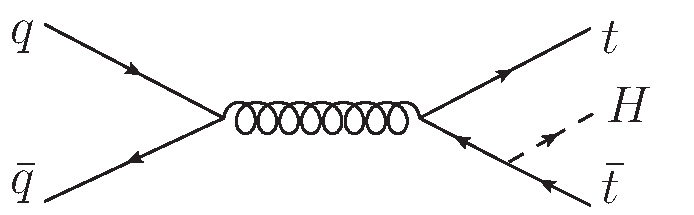
\includegraphics[scale=0.45]{qqs1_II.pdf}}
\hspace*{0.05\textwidth}
%\label{fig1a}}
\subfloat{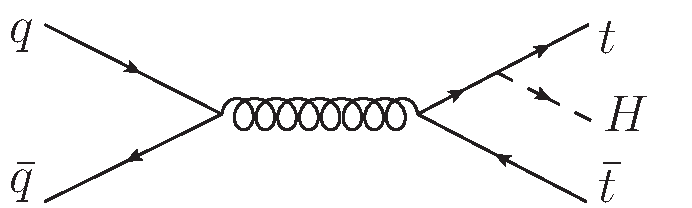
\includegraphics[scale=0.45]{qqs2_II.pdf}}
%\label{fig1b}}
\\[0.032\textwidth]
\subfloat{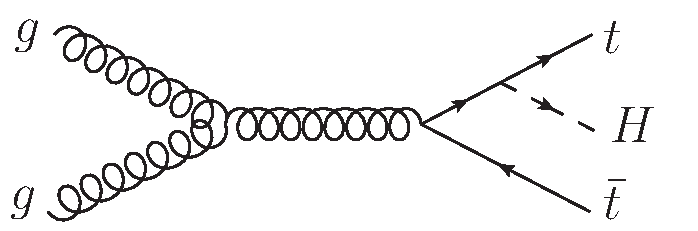
\includegraphics[scale=0.45]{ggs1_II.pdf}}
\hspace*{0.05\textwidth}
%\label{fig1b}}
\subfloat{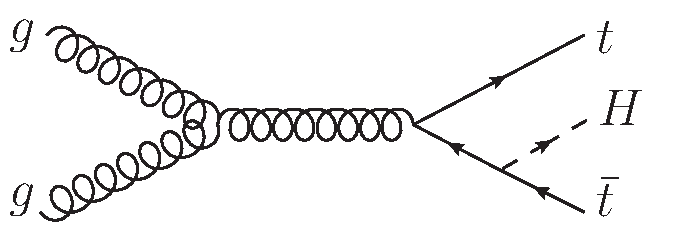
\includegraphics[scale=0.45]{ggs2_II.pdf}}
%\label{fig1c}}
\\[0.032\textwidth]
\subfloat{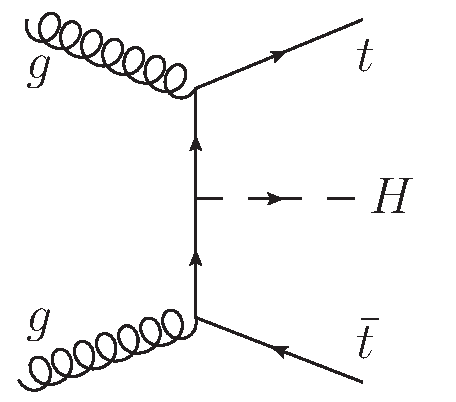
\includegraphics[scale=0.45]{ggt1_II.pdf}}
%\label{fig1b}}
\hspace*{0.025\textwidth}
\subfloat{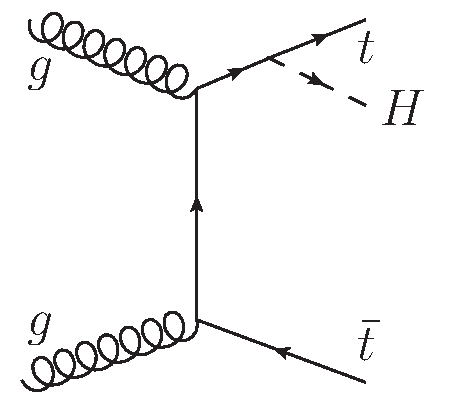
\includegraphics[scale=0.45]{ggt2_II.pdf}}
%\label{fig1c}}
\hspace*{0.025\textwidth}
\subfloat{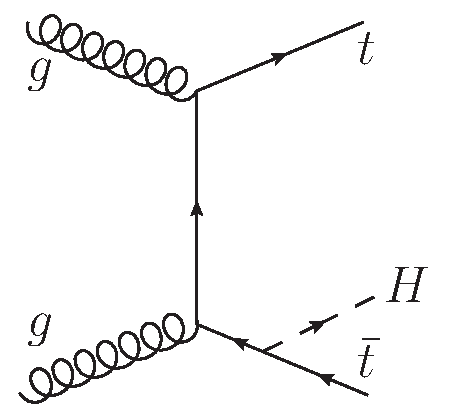
\includegraphics[scale=0.45]{ggt3_II.pdf}}
%\label{fig1b}}
\vspace*{0.02\textwidth}
\caption{Tree-level Feynman diagrams contributing to $t\tbar H$ production
  at the LHC. Three more diagrams are obtained by exchanging the gluon
  lines in the $t$-channel diagrams.}
\label{fig1}
\end{figure}
\end{center}
%%%%%%%%%%%%%%%%%%%%%%%%%%%%%%%%%%%%%%%%%%%%%%%%%%%%%%%%%%%%
\subsection{Factorized expression for the scattering cross section}
\label{subsec:factorize}

In this subsection we focus on the gluon fusion
{\bf (KK: seems repetitive to say ``gluon fusion'' right away
  again\ldots maybe can change this; maybe OK to leave it?)}
contributions
to $t\tbar H$ production, since these dominate over the
the quark-antiquark annihilation contributions.  Furthermore,
we consider the case in which the top and antitop both decay
semileptonically.  As we shall show below, assuming the
narrow width approximation for the top and antitop quarks, the unpolarized
differential cross section for $gg\to t(\to
b{\ell}^+\nu_{\ell})\,\tbar(\to \bbar {\ell}^- \nubar)\,H$ may be
written in the following ``factorized'' form,\footnote{The reader
  is referred to the discussion following Eq.~(\ref{eq17}) for some qualifying
  remarks regarding the ``factorization'' of this expression.}
%
\beq
\label{eq2}
%dd\sigma(gg\to (bl^+\nu_l)(\bbar l^- \nubar) H)=\sum_{\substack{bl^+\nu_l \\ \tiny{\mathrm{spins}}}}\,\sum_{\substack{\bbar l^-\nubar \\ \mathrm{\tiny{spins}}}}\left(\frac{2}{\Gamma_t}\right)^2\,d\sigma(gg\to t(n_t)\tbar (n_{\tbar})H)\,d\Gamma(t(n_t)\to bl^+\nu_l)\,d\Gamma(\tbar (n_{\tbar})\to \bbar l^-\nubar)
d\sigma =\sum_{\substack{b{\ell}^+\nu_l \\ \tiny{\mathrm{spins}}}}\,
   \sum_{\substack{\bbar {\ell}^-\nubar \\ \mathrm{\tiny{spins}}}}\left(\frac{2}{\Gamma_t}\right)^2\,
   d\sigma(gg\to t(n_t)\tbar (n_{\tbar})H)\,
   d\Gamma(t\to b{\ell}^+\nu_{\ell})\,
   d\Gamma(\tbar \to \bbar {\ell}^-\nubar),
\eeq  
%
where $d\sigma(gg\to t(n_t)\tbar (n_{\tbar})H)$ is the differential
cross section for the production of a top and antitop quark,
with spin vectors $n_t$ and $n_{\bar{t}}$, respectively, along with a Higgs
boson.  Also, $d\Gamma(t\to b{\ell}^+\nu_{\ell})$ and
$d\Gamma(\tbar \to \bbar {\ell}^-\nubar)$ are the
partial differential decay widths for an unpolarized top and
anti-top quark.  The four-vectors
$n_t$ and $n_{\tbar}$ are not arbitrary, but are
given by particular combinations of the
momenta of the $t,\tbar, \ell^+$ and $\ell^-$~\cite{Arens},
%
\bea
\label{eq3}
n_t&=&-\frac{p_t}{m_t}+\frac{m_t}{(p_t\cdot p_{{\ell}^+})}p_{{\ell}^+}\\
\label{eq4}
n_{\tbar}&=&\,\frac{p_{\tbar}}{m_t}-\frac{m_t}{(p_{\tbar}\cdot p_{{\ell}^-})}p_{{\ell}^-}.
\eea
%
Expressions similar to Eq.~(\ref{eq2}) have been derived previously for the
production of short-lived particles in $e^-e^+$ colliders
\cite{kawasaki} and for $t\tbar$ production both in
$e^-e^+$ colliders \cite{Arens} and $pp$ colliders
\cite{ale1,*ale2,*ale3,*ale4}. \par

%%%%%%%%%%%%%%%%% FIGURA 2 %%%%%%%%%%%%%%%%%%%%%%
\begin{center}
\begin{figure}[H]
\centering
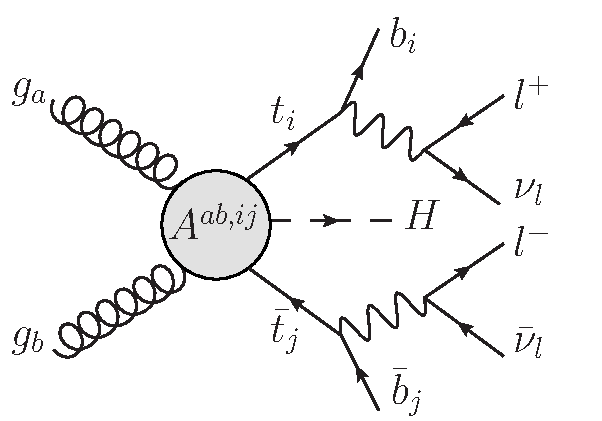
\includegraphics[scale=0.6]{esquematico_II.pdf}
\vspace*{0.02\textwidth}
\caption{Schematic representation of the process $g_ag_b\to t(\to
  b_i{\ell}^+\nu_{\ell})\tbar(\to \bbar_j {\ell}^- \nubar) H$. The
  indices $i,j$ denote the colour of the quarks while $a,b$ are gluon
  indices.}
\label{fig2}
\end{figure}
\end{center}
%%%%%%%%%%%%%%%%%%%%%%%%%%%%%%%%%%%%%%%%%%%%%%%%%

To derive the above expressions, we begin by considering the
schematic representation for the process $g_ag_b\to t(\to
b_i{\ell}^+\nu_{\ell})\,\tbar(\to \bbar_j {\ell}^- \nubar)\,H$
that is sketched in Fig.~\ref{fig2}.
Here $a$ and $b$ denote the initial-state gluons and
$i$ and $j$ refer to the colours of the top and antitop quarks.
%\par
%
The amplitude for this process may be written in the following
compact form
%
\beq
\label{eq6}
\mathcal{M}^{ab,ij}=\bar{\psi}_t\,\mathcal{A}^{ab,ij}\,\psi_{\tbar}\,,
\eeq
%
where the spinors $\bar{\psi}_t$ and $\psi_{\tbar}$
contain all of the information regarding the decay of the
virtual top and anti-top, respectively,
and where the quantity $A^{ab,ij}$ is given by
%
\beq
\label{eq5}
\mathcal{A}^{ab,ij}\equiv A^{ab,ij}_{\mu\nu}(\epsilon_{\lambda_a})^{\mu}(\epsilon_{\lambda_b})^{\nu}=\sum_{k=1}^8 \mathcal{A}^{ab,ij}_k =\kp \sum_{k=1}^8 \mathcal{S}^{ab,ij}_k + i\kpt \sum_{k=1}^8 \mathcal{P}^{ab,ij}_k.
\eeq 
%
The sum over $k$ in the above expression
corresponds to the eight gluon-initiated
diagrams indicated in Fig.~\ref{fig1}; also,
$\epsilon_{\lambda_a}$ and $\epsilon_{\lambda_b}$ are the
polarization vectors corresponding to $g_a$ and $g_b$, respectively.
In the last equality in Eq.~(\ref{eq5})
we have explicitly separated the amplitude into
two sums, with one sum corresponding to the scalar contributions
and the other to the pseudoscalar ones.
Taking all of the final-state particles to be massless, we can use the
spinor techniques
developed in \cite{Kleiss} to write $\bar{\psi}_t$ and
$\psi_{\tbar}$ as follows\footnote{These spinor techniques can also be used
  for massive final-state particles. Given the
  energy scale involved in the process in question, however, the assumption
  of massless final-state particles is sensible and greatly
  simplifies the derivation of Eq.~(\ref{eq2}).}
%
\bea
\label{eq7}
\bar{\psi}_t &=& -g^2\, \mathbb{P}_t(t)\,\mathbb{P}_W(t-b)\,
   \langle b-|\nu_{\ell}+\rangle \langle {\ell}^+\!+|(\tslash+m_t)\\
\label{eq8}
\psi_{\tbar} &=& g^2\, \mathbb{P}_t(\tbar)\,\mathbb{P}_W(\tbar-\bbar)\,
   \langle\nubar+|\bbar-\rangle (\tbslash-m_t)|{\ell}^-+\rangle,
\eea
%
where $|i+(-)\rangle \equiv (1/2)(1\pm \gamma^5)\,\psi_i$
represents a right-handed (left-handed) chiral spinor for final-state
particle $i$ and $\langle i+(-)|$ represents the corresponding adjoint spinor.
Also, $\mathbb{P}_t(q)=(q^2-m^2_t+im_t\Gamma_t)^{-1}$ and
$\mathbb{P}_W(q)=(q^2-m^2_W+im_W\Gamma_W)^{-1}$, and
we have denoted the momenta of the various particles by the symbols
that refer to the names of those particles~\cite{Mangano}.

Using the expressions defined above for $\bar{\psi}_t$ and
$\psi_{\tbar}$, we can write the amplitude $\mathcal{M}^{ab,ij}$
in a form that is (in a sense) factorized.
As a first step, we insert
Eqs.~(\ref{eq7}) and (\ref{eq8}) into Eq.~(\ref{eq6}), yielding
%
\beq
\label{eq9}
\mathcal{M}^{ab,ij}=\!-g^4\,\mathbb{P}_t(t)\,\mathbb{P}_t(\tbar)\,\mathbb{P}_W(t-b)\,\mathbb{P}_W(\tbar-\bbar)\,\langle b-|\nu_{\ell}+\rangle \langle\nubar+|\bbar-\rangle \sqrt{\strut2(t\cdot {\ell}^+)}\sqrt{\strut2(\tbar\cdot {\ell}^-)}\,[\bar{\phi}_t \mathcal{A}^{ab,ij}\phi_{\tbar}],
%\frac{1}{(t^2-m^2_t+im_t\Gamma_t)}\,\frac{1}{(\tbar^2-m^2_t+im_t\Gamma_t)}\,\frac{1}{((t-b)^2-M^2_W)}\frac{1}{((\tbar-\bbar)^2-M^2_W)}\,\langle b-|\nu+\rangle\,\langle\nubar+|\bbar-\rangle
\eeq
%
where the spinors $\phi_{t}$ and $\phi_{\tbar}$ are defined as
%
\beq
\label{eq10}
\phi_t=\frac{(\tslash +m_t)}{\sqrt{\strut2(t\cdot {\ell}^+)}}|{\ell}^++\rangle
\eeq
%
\beq
\label{eq11}
\phi_{\tbar}=\frac{(\tbslash -m_t)}{\sqrt{\strut2(\tbar\cdot {\ell}^-)}}|{\ell}^-+\rangle \,.
\eeq
%
Note that in writing down the above expressions we have adopted the narrow-width
approximation for the top and antitop quarks and for the $W^\pm$ gauge
bosons.\footnote{Since Eq.~(\ref{eq9}) contains the top quark propagator
  term
  $\mathbb{P}_t(t)$, for example, $|\mathcal{M}^{ab,ij}|^2$ contains
  the factor $((t^2-m^2_t)^2+m^2_t\Gamma^2_t)^{-1}$,
  which is replaced by $(\pi/m_t\Gamma_t)\delta(t^2-m^2_t)$
  in the narrow-width approximation.  Thus, except for the propagator terms $\mathbb{P}_t(t)$ and $\mathbb{P}_t(\tbar)$,
   we take the four-vector $t$ appearing in Eqs.~(\ref{eq9})-(\ref{eq11}) to be
  on shell, satisfying $t^2 = m_t^2$.} 
Working out the projection operators $\phi_t\,\bar{\phi}_t$
and $\phi_{\tbar}\,\bar{\phi}_{\tbar}$, we have
%
\beq
\label{eq12}
\phi_t\,\bar{\phi}_t=\frac{1}{2}(1+\nslash_{\!t}\gamma^5)(\tslash +m_t)
\eeq
%
and
%
\beq
\label{eq13}
\phi_{\tbar}\,\bar{\phi}_{\tbar}=\frac{1}{2}(1+\nslash_{\!\tbar}\gamma^5)(\tbslash -m_t),
\eeq
%
with $n_t$ and $n_{\tbar}$ being the four-vectors defined in
Eqs.~(\ref{eq3}) and (\ref{eq4}).  Thus, $\phi_t$ and $\phi_{\tbar}$
may be regarded as
describing a top quark with spin vector $n_t$ and an antitop quark
with spin vector $n_{\tbar}$, respectively.

As a final step toward factorizing the amplitude $\mathcal{M}^{ab,ij}$,
we note that the amplitude for a top quark with spin vector
$n_t$ to decay into $b{\ell}^+\nu_{\ell}$ is given by
%
\beq
\label{eq14}
\mathcal{M}(t(n_t)\to b{\ell}^+\nu_{\ell})=ig^2\mathbb{P}_W(t-b)\langle b-|\nu_{\ell}+\rangle\sqrt{\strut2(t\cdot {\ell}^+)} \,,
\eeq
%
and likewise,
%
\beq
\label{eq15}
\mathcal{M}(\tbar(n_{\tbar})\to \bar{b}{\ell}^-\bar{\nu}_{\ell})=ig^2\mathbb{P}_W(\tbar-\bar{b})\langle \bar{\nu}_{\ell}+|\bar{b}-\rangle\sqrt{\strut2(\tbar\cdot {\ell}^-)}.
\eeq
%
Furthermore, the term inside the square brackets in
Eq.~(\ref{eq9}) is the amplitude for producing a top quark
with spin vector $n_t$, along with an anti-top with spin vector
$n_{\tbar}$ and a Higgs boson,
%
\beq
\label{eq16}
\mathcal{M}(g_ag_b \to t^i(n_t)\tbar^j(n_{\tbar})H)=\bar{\phi}_t \mathcal{A}^{ab,ij}\phi_{\tbar}.
\eeq
%
Combining Eqs.~(\ref{eq14})-(\ref{eq16}), we can write Eq.~(\ref{eq9})
in a form that appears to be factorized,
%
\beq
\label{eq17}
\mathcal{M}^{ab,ij}=\mathbb{P}_t(t)\mathbb{P}_t(\tbar)\,\mathcal{M}(t(n_t)\to b{\ell}^+\nu_{\ell})\,\mathcal{M}(\tbar(n_{\tbar})\to \bar{b}{\ell}^-\bar{\nu}_{\ell})\,\mathcal{M}(g_ag_b \to t^i(n_t)\tbar^j(n_{\tbar})H) \,.
\eeq
%
It is important
to note that, even though the above expression has the appearance of being
factorized into production and decay parts, this apparent
factorization is a bit misleading.  In particular, the amplitude for
$t\tbar H$ production contains the top and antitop quark
spin four-vectors $n_t$ and $n_{\tbar}$, which
depend on final-state kinematical quantities [see
Eqs.~(\ref{eq3}) and (\ref{eq4})].
With this qualification in mind, we may now use the
amplitude in Eq.~(\ref{eq17})
to determine the corresponding scattering cross section.
After some manipulation of the phase space variables
to take advantage of the presence of the
propagator terms, $\mathbb{P}_t(t)$ and $\mathbb{P}_t(\tbar)$,
we arrive at the expression in Eq.~(\ref{eq2}).\footnote{The reader may note that in the differential widths of $t\to b{\ell}^+\nu_{\ell}$ and $\tbar\to \bar{b}{\ell}^-\bar{\nu}_{\ell}$ appearing in 
Eq.~(\ref{eq2}), the spin states of the top an antitop have been averaged. Interestingly, under the assumption of massless final-state particles, the amplitudes $\mathcal{M}(t(-n_t)\to b{\ell}^+\nu_{\ell})$ and $\mathcal{M}(\tbar(-n_{\tbar})\to \bar{b}{\ell}^-\bar{\nu}_{\ell})$ vanish. } This expression
also has the appearance of being factorized, but
qualifying remarks, similar to those above, apply.

%%%%%%%%%%%%%%%%%%% Quitarlo %%%%%%%%%%%%%%%%%%%%
\setlength{\abovedisplayskip}{10.2pt}
\setlength{\belowdisplayskip}{10.2pt}
%%%%%%%%%%%%%%%%%%%%%%%%%%%%%%%%%%%%%%%%%%%%%%%%%

\subsection{Origin of triple product terms}
\label{subsec:origin}

The expression derived above for the scattering cross
section [see Eq.~(\ref{eq2}), as well as Eq.~(\ref{eq17})]
provides significant insight into
how one might analyze $\ppprocess$ in order to determine
the nature of the top-Higgs coupling.  In particular,
let us focus on the production amplitude,
$\mathcal{M}(g_ag_b \to t^i(n_t)\tbar^j(n_{\tbar})H))$, which forms
part of the overall amplitude in Eq.~(\ref{eq17}).
The absolute value squared of the production amplitude
is used to determine $d\sigma(gg\to t(n_t)\tbar (n_{\tbar})H)$,
which in turn forms part of the expression for the ``factorized'' cross section
in Eq.~(\ref{eq2}).  Summing over colour and gluon indices
we have
%
\beq
\label{eq18}
\sum_{\substack{a,b \\ i,j}}|\mathcal{M}(g_ag_b \to t^i(n_t)\tbar^j(n_{\tbar})H)|^2=\sum_{\substack{a,b \\ i,j}}\left|\sum^{8}_{k=1}C^{ab,ij}_k\,\bar{\phi}_t (\kp\mathcal{S}_k+i\kpt\mathcal{P}_k)\phi_{\tbar}\right|^2,
\eeq
%
where we have separated the colour structure of each diagram by defining
$\mathcal{S}^{\,ab,ij}_k= C^{ab,ij}_k \mathcal{S}_k$ and
$\mathcal{P}^{\,ab,ij}_k= C^{ab,ij}_k \mathcal{P}_k$
[see Eqs.~(\ref{eq5}) and (\ref{eq16})]. Also, the factors
$g^2_s m_t/v$ and $-ig^2_s m_t/v$ arising from the vertices of the $t$-
and $s$-channel diagrams respectively have been included in the
definition of $C^{ab,ij}_k$ for convenience. The terms linear in $\kp$
and $\kpt$ can be written as
%
\beq
\label{eq19}
\mathcal{O}(\kp\kpt)\to \frac{1}{2}\kp\kpt \sum_{k,r}\mathbb{C}_{kr}\mathrm{Im}
\left\lbrace \mathrm{Tr}\left[ (1+\nslash_t \gamma^5)(\tslash+m_t)\mathcal{S}_k(1+\nslash_{\tbar}\gamma^5
 )(\tbslash -m_t)\tilde{\mathcal{P}}_r \right] \right\rbrace ,
\eeq
%
where the factor $\mathbb{C}_{kr}=\sum_{ab,ij}C^{ab,ij}_k
C^{ab,ij*}_r$ is real and where $\tilde{\mathcal{P}}_r = \gamma^0
\mathcal{P}^{\dagger}_r \gamma^0$.
The only terms that yield non-zero contributions
in the above sum are those with an
odd number of $\gamma^5$ matrices; these lead to triple-product
(TP) structures
of the form $\epsilon_{\alpha\beta\gamma\delta}\,p^{\alpha}_ap^{\beta}_bp^{\gamma}_cp^{\delta}_d$,
where $p_a$-$p_d$ represent various four momenta associated with the process.
In contrast,
it can be seen from Eq.~(\ref{eq18}) that the terms proportional to
$\kp^2$ and $\tilde{\kappa}^2_t$ descend from traces containing
an even number of $\gamma^5$
matrices and can be written in terms of scalar products of the
available momenta.\par
%\vspace*{-2mm}

With the above considerations in mind, it is useful to
write a general expression for the differential cross
section $d\sigma(gg\to t(n_t)\tbar (n_{\tbar})H)$
in terms of the momenta $q=(q_1-q_2)/2$,
$Q=(q_1+q_2)/2$, $t$, $\bar{t}$, $n_t$ and $n_{\tbar}$, where
$q_{1,2}$ denote the momenta of the initial-state gluons. Note that with this
choice, $q\cdot Q=0$ and $Q^2=-q^2=M^2_{t\tbar H}/4$, where $M_{t\tbar
  H}$ is the invariant mass of the $t\tbar H$ system.
Fifteen TPs can be constructed from these six
four-vectors,\footnote{We note that these fifteen
  TPs are not linearly independent (see the epsilon relations
  discussed in Ref.~\cite{identities}).} so that
%
\beq
\label{eq20}
d\sigma(gg\to t(n_t)\tbar (n_{\tbar})H)= \kp^2\,f_1(p_i\cdot p_j)+\tilde{\kappa}^2_t\,f_2(p_i\cdot p_j)+\kp\kpt\,\sum^{15}_{l=1}g_l(p_i\cdot p_j)\,\epsilon_l,
\eeq   
%
where
$\epsilon_l=\epsilon_{\alpha\beta\gamma\delta}\,p^{\alpha}_ap^{\beta}_bp^{\gamma}_cp^{\delta}_d$
denotes the $l$th TP (we adopt the convention $\epsilon_{0123}=+1$) and where $p_i$ and $p_j$ refer to any of the
six momenta.  The
functions $f_{1,2}$ and $g_k$ depend only on the possible scalar
products and are therefore even under a parity transformation
($\mathrm{P}$). However, the terms linear in $\kp\kpt$ are
$\mathrm{P}$-odd due to the presence of the $\mathrm{P}$-odd
TPs. Hence, only the functions $f_{1,2}$ will contribute to the total
cross-section, whereas the TP terms will be sensitive to the sign of
the anomalous coupling $\kpt$. Of the fifteen TPs mentioned above,
we will focus on those that contain both of the spin
vectors $n_t$ and $n_{\tbar}$, but do not include $q$.
The decision not to consider $q$-dependent TPs is motivated by the fact
that $q$ cannot be expressed in terms of the momenta of final state
particles (as $Q$ can, by virtue of energy-momentum conservation). The
decision to focus on TPs that contain both $n_t$ and $n_{\tbar}$
is rooted in the fact that the spins of pair-produced top and antitop quarks
are highly correlated at hadron colliders 
(even though the quarks themselves are unpolarized).
Observables that combine the decay products of the
$t$ and $\tbar$ will be sensitive to this spin
correlation~\cite{Bernreuther}.  A similar behaviour is expected in $t\tbar H$
production, where it can be shown that single-spin asymmetries
vanish~\cite{Ellis,Biswas}. Hence, in order to construct observables
sensitive to the structure of the $tH$ coupling, we will restrict our attention
to those
TPs that include information on the decay products of both the top and
anti-top quarks. Only five of the fifteen TPs in Eq.~(\ref{eq20}) do
not involve the four vector $q$ and, among these, only three
include both $n_t$ and $n_{\tbar}\,$.  Thus, we will restrict our attention
to the following TPs
%
\beq
\label{eqa1}
\epsilon_1\equiv\epsilon(t,\tbar,n_t,n_{\tbar}),\,\,
\vspace*{1mm}
\eeq
%
\beq
\label{eqa2}
\epsilon_2\equiv\epsilon(Q,\tbar,n_t,n_{\tbar}),
\vspace*{1mm}
\eeq
%
\beq
\label{eqa3}
\epsilon_3\equiv\epsilon(Q,t,n_t,n_{\tbar}).
\vspace*{1mm}
\eeq
%
\par  

Before turning to a consideration of various CP-odd observables,
we remark that even though all of the above discussion took place
within the context of $gg$-initiated production, similar conclusions
are obtained for $q\qbar$-initiated production. In particular, the
definitions of the spin vectors in Eqs.~(\ref{eq3})-(\ref{eq4}) and
the general form of $d\sigma$ introduced in Eq.~(\ref{eq20}) are valid
in both cases.
%%%%%%%%%%%%%%%%%%%%%%%%%%%%%%%%%%%%%%%%%%%%%%%%%
%\newpage
%%%%%%%%%%%%%%%%%%%%%%%%%%%%%%%%%%%%%%%%%%%%%%%%%
%\setlength{\belowdisplayskip}{10pt} \setlength{\belowdisplayshortskip}{10pt}
%\setlength{\abovedisplayskip}{10pt} \setlength{\abovedisplayshortskip}{10pt}
\bigskip
\section{$\mathrm{\mathbf{CP}}$-odd observables}
\label{sec3}
In this section we present three types of observables based on the TPs discussed
in Sec.~\ref{sec2}, namely, asymmetries, angular
distributions and mean values. These observables are sensitive not only to the
magnitude of the pseudoscalar coupling $\kpt$, but also to its
sign.  In order to test the various observables, we have
used $\mathtt{MadGraph5\_aMC@NLO}$ \cite{Madgraph} to simulate the process
$\ppprocess$ at parton level for different values of the couplings
$\kp$ and $\kpt$.  In all cases we have generated $10^5$ events
and have assumed a center-of-mass energy of
$14\,\mathrm{TeV}$.\footnote{Note that, since we generate
  the same number of events in
  each case, the corresponding integrated luminosities are different, since the
  cross section depends on the value of $\kpt$.}
We have also imposed the
following set of cuts: $p_T$ of leptons $> 10\,\mathrm{GeV}$, $|\eta|$
of leptons $< 2.5$, $|\eta|$ of b jets $< 2.5$ and $\Delta
R_{\ell\ell}>0.4$.  Note that we have used this
somewhat large number of events ($10^5$) in order to determine clearly
the extent to which the proposed observables are sensitive to the NP
coupling.  Section~\ref{sec6} contains an
analysis of the experimental feasibility of the more promising observables.

Before continuing on to our analysis, let us make a few comments
regarding the values that we choose for $\kp$ and $\kpt$.
First of all, we note that if the pseudoscalar
coupling $\kpt$ is the only source of physics beyond the SM,
then indirect contraints (based on the signal strength of $gg\to H \to \gamma\gamma$) 
disfavour $\kp < 0$ but do not
resolve the degeneracy in the sign of $\kpt$ \cite{Guadagnoli}. On
the other hand, if one assumes that the tensor structure of the
Higgs interactions are the
same as those of the SM and if one parameterizes these interactions via
one universal Higgs coupling to vector bosons, $\kappa_V$, and one
universal Higgs coupling to fermions, $\kappa_f$, then the measured signal
strengths provided by the ATLAS and CMS collaborations are compatible with
the values predicted by the SM, (namely, $\kappa_f=1$ and $\kappa_V=1$).
With these facts in mind, we will, for the most part,
set the value of the scalar coupling to its SM
value ($\kp=1$) and will allow the pseudoscalar coupling to take on
various values (including both possible signs). In particular, we
analyze the cases $\kpt=0,\pm 0.25, \pm 0.5, \pm 0.75,\pm 1$.
In addition, we also provide some analysis regarding the pure
$\mathrm{CP}$-odd case ($\kp=0,\kpt=1$).
%\newpage
%%%%%%%%%%%%%%%%%%%%%%%%%%%%%%%%%%%%%%%%%%%%%%%%%
\subsection{Asymmetry}
%\bigskip
\label{sec3.1}

The first type of $\mathrm{CP}$-odd observable that we will consider is an
asymmetry that compares the number of events
for which a given TP is positive to that for which it is negative.
Normalizing to the total number of events, we define
%
\beq
\label{eq21}
\mathcal{A}(\epsilon)=\frac{N(\epsilon > 0)-N(\epsilon < 0)}{N(\epsilon > 0)+N(\epsilon < 0)}.
\eeq 
%
By construction, $\mathcal{A}\in [-1,+1]$.
Based on the general expression given in Eq.~(\ref{eq20}), we expect
the following functional form for the asymmetry,
%
\beq
\label{eq22}
\mathcal{A}(\epsilon)=\frac{A\kp\kpt}{B\kappa^2_t+C\tilde{\kappa}^2_t},
\eeq 
%
which for $\kp=1$ can be parameterized as
%
\beq
\label{eq23}
\mathcal{A}(\epsilon)=\frac{a\kpt}{1+b\tilde{\kappa}^2_t},
\eeq 
%
where the parameter $a\equiv A/B$ determines the sensitivity to the
pseudoscalar coupling, whereas $b\equiv C/B$ quantifies the deviation
from linear behaviour.

Table~\ref{table1} shows numerical results for the
asymmetries associated with three different TPs,
$\epsilon_1$, $\epsilon_2$ and $\epsilon_3$, taking
$\kp=1$ and $\kpt=0,\pm 1$.  The asymmetry $\mathcal{A}$
is shown in each case, along with $\mathcal{A}/\sigma_{\mathcal{A}}$, where
$\sigma_{\mathcal{A}}$ is the corresponding
statistical uncertainty.  As is
evident from the table, the asymmetries in question provide
a clear separation between the SM and the 
$\mathrm{CP}$-mixed cases, with typical deviations being of
order $10\sigma$.  Furthermore, the asymmetries
for the SM case are each statistically consistent with zero,
as one would expect.
The three asymmetries also allow one to
determine the sign of $\kpt$,
with deviations between the $\kpt = \pm 1$ cases typically
being of order $20\sigma$.
{\bf (We couldn't figure out how to clarify this. If you find a way go ahead\ldots.)}
The sensitivity of
the asymmetry is quite similar for the three TPs, as can be seen by
including other values of $\kpt$ and using the expression in
Eq.~(\ref{eq23}) as a fitting function (see Fig.~\ref{fig3}).
Performing such a fit, 
we obtain $(a=-0.057\pm 0.006, b=0.5\pm 0.2),
(a=-0.056\pm 0.006, b=0.5 \pm 0.2)$ and $(a=0.058\pm 0.006, b=0.6 \pm
0.2)$ for $\epsilon_1$, $\epsilon_2$ and $\epsilon_3$,
respectively.

The results shown in Table~\ref{table1}
and Fig.~\ref{fig3} all assume a $pp$ initial state, which is
actually a combination of events coming from $gg$ and $q\qbar$
initial states.
While this combination of initial states is the appropriate scenario
to consider, it
is interesting to consider the relative contributions to the asymmetry
coming from the
$gg$ and $q\qbar$ initial states.  Figure~\ref{fig4} shows
three curves for the ``$\epsilon_1$'' case, one for $gg$-initiated
events, one for $q\qbar$-initiated events, and one for the usual
combination of these events (the ``$pp$'' initial state).
Interestingly, we see from Fig.~\ref{fig4} that the asymmetry for this TP
is enhanced for
$gg$-initiated production, while it is reduced and of opposite sign
for the $q\qbar$-initiated events. The asymmetry for the $pp$ case is
evidently
dominated by the $gg$ contribution, but is somewhat smaller
in magnitude due to the
$q\qbar$ contribution.
\newcolumntype{C}[1]{>{\centering\arraybackslash}p{#1}}
\renewcommand{\arraystretch}{1.4}
\begin{table}[H]
  \caption{Asymmetries for three different scenarios,
    obtained by using $10^5$ simulated events for the
    TPs $\epsilon_1=\TPa, \epsilon_2=\TPb$ and $\epsilon_3=\TPc$.
    The three scenarios
  correspond to the SM ($\kp=1$ and $\kpt=\pm 0$) and
  two $\mathrm{CP}$-mixed cases (defined by
  $\kp=1$ and $\kpt=\pm 1$).}
\label{table1}
\begin{center}
\begin{tabular}{|C{1cm}|C{1cm}||C{2cm}|C{2cm}||C{2cm}|C{2cm}||C{2cm}|C{2cm}|}
%\begin{tabular}{|c|r||r|c||r|c||r|c|}
\hhline{|========|}
%\hhline{|--------|}
$\kappa_t$&$\tilde{\kappa}_t$~~&$\mathcal{A}(\epsilon_1)$~~&$\mathcal{A}(\epsilon_1)/\sigma_{\mathcal{A}}$& $\mathcal{A}(\epsilon_2)$~~&$\mathcal{A}(\epsilon_2)/\sigma_{\mathcal{A}}$&$\mathcal{A}(\epsilon_3)$~~&$\mathcal{A}(\epsilon_3)/\sigma_{\mathcal{A}}$  \\ 
\hhline{|========|} 
%\hhline{|--------|}
$1$ & $-1$~~~ & $0.0315$~ & $10.0$ & $0.0332$~ & $10.5$~ & $-0.0307$~~~ & $-9.7$~~~\\[0.6mm]
\hline
$1$ & $0$ & $-0.0021$~~~ & $-0.7$~~~ & $0.0009$~ & $0.3$~ & $-0.0011$~~~ & $-0.3$~~~\\[0.6mm]
\hline
$1$ & $1$ & $-0.0379$~~~ & $-12.0$~~~ & $-0.0411$~~~& $-13.0$~~~ & $\,0.0378$~ & $12.0$ \\[0.6mm]
\hhline{|========|}
%\hhline{|--------|}
\end{tabular}
\end{center} 
\end{table}
%%%%%%%%%%%%%%%%%%%%%%%%% FIGURA 3 %%%%%%%%%%%%%%%%%%%%%%%%%
\begin{center}
\vspace*{2.5mm}
\begin{figure}[H]
%\centering
\hspace*{-0.45cm}
\subfloat{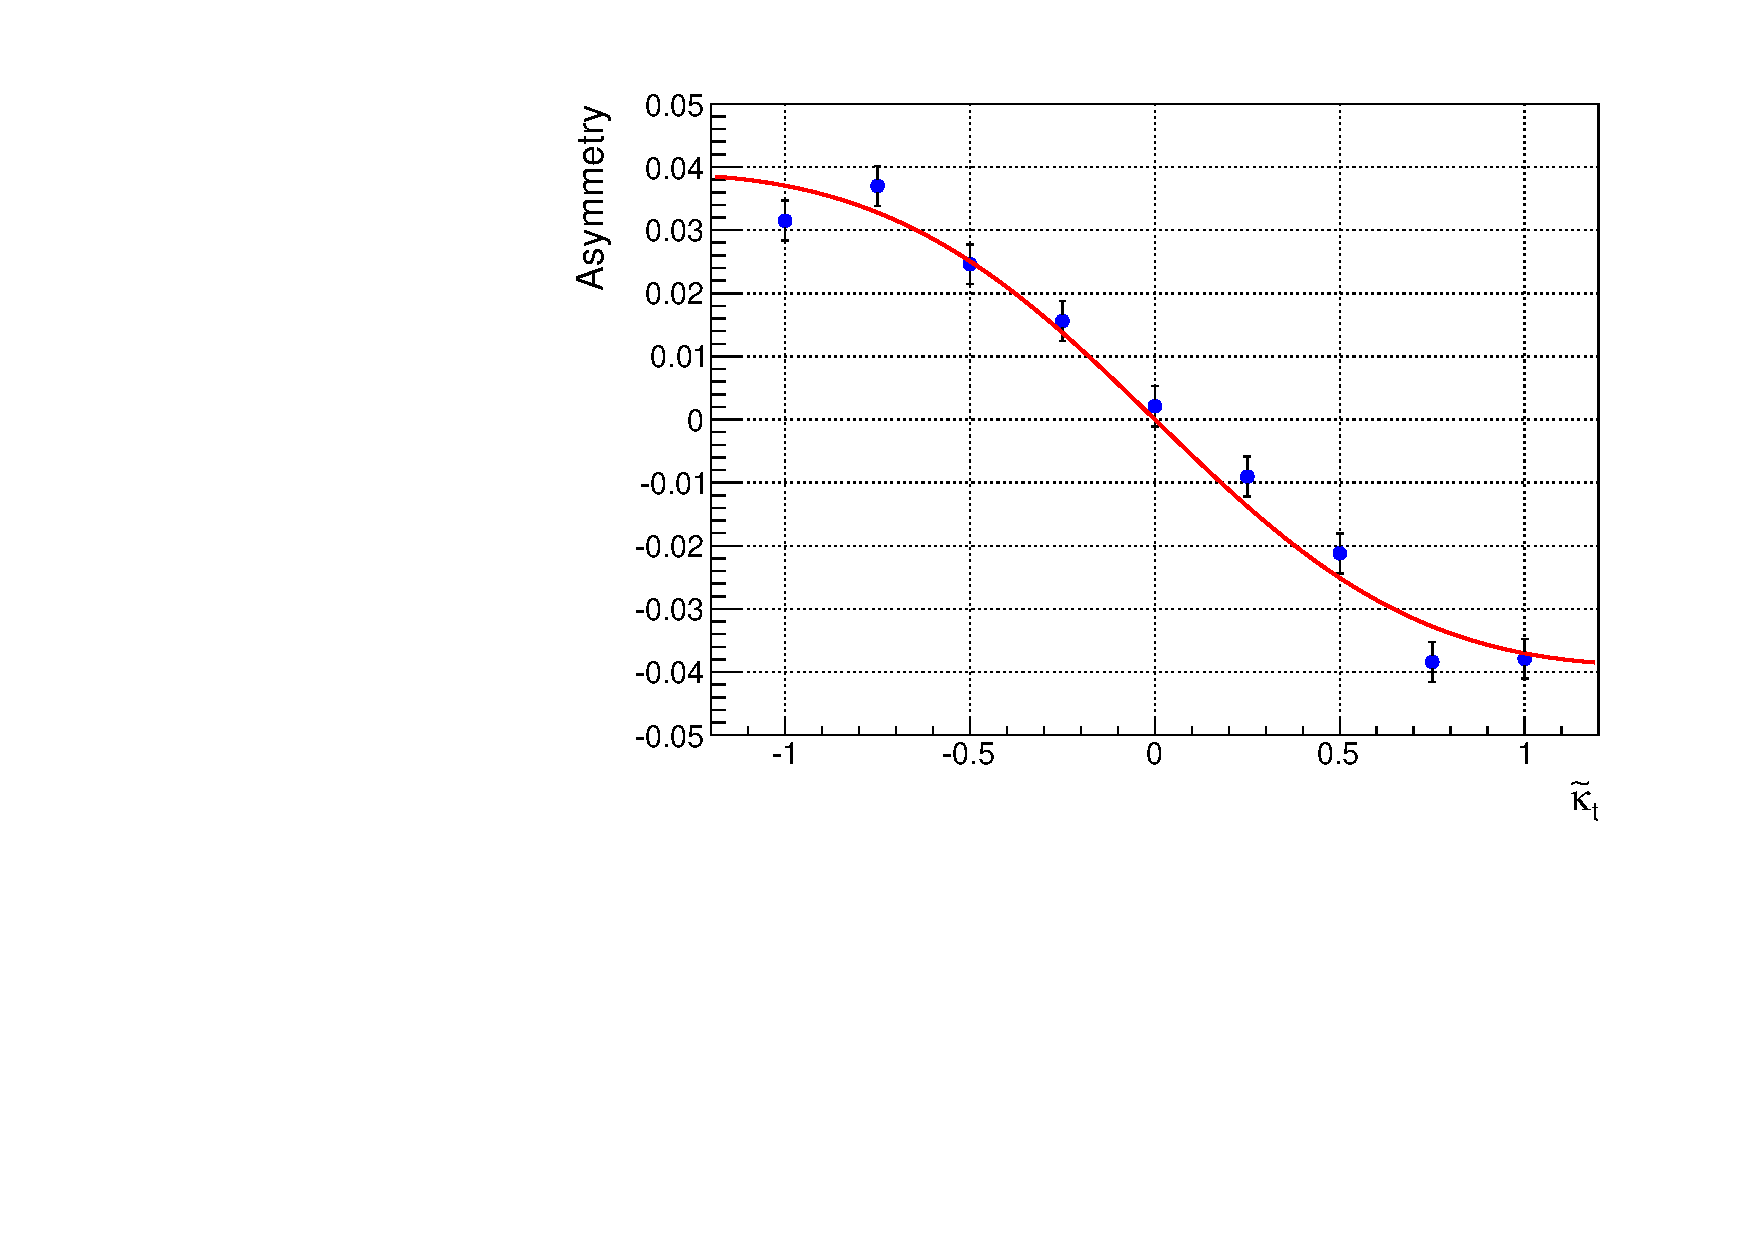
\includegraphics[scale=0.45]{ATP1_nuevo.pdf}}
\hspace*{0.002\textwidth}
\subfloat{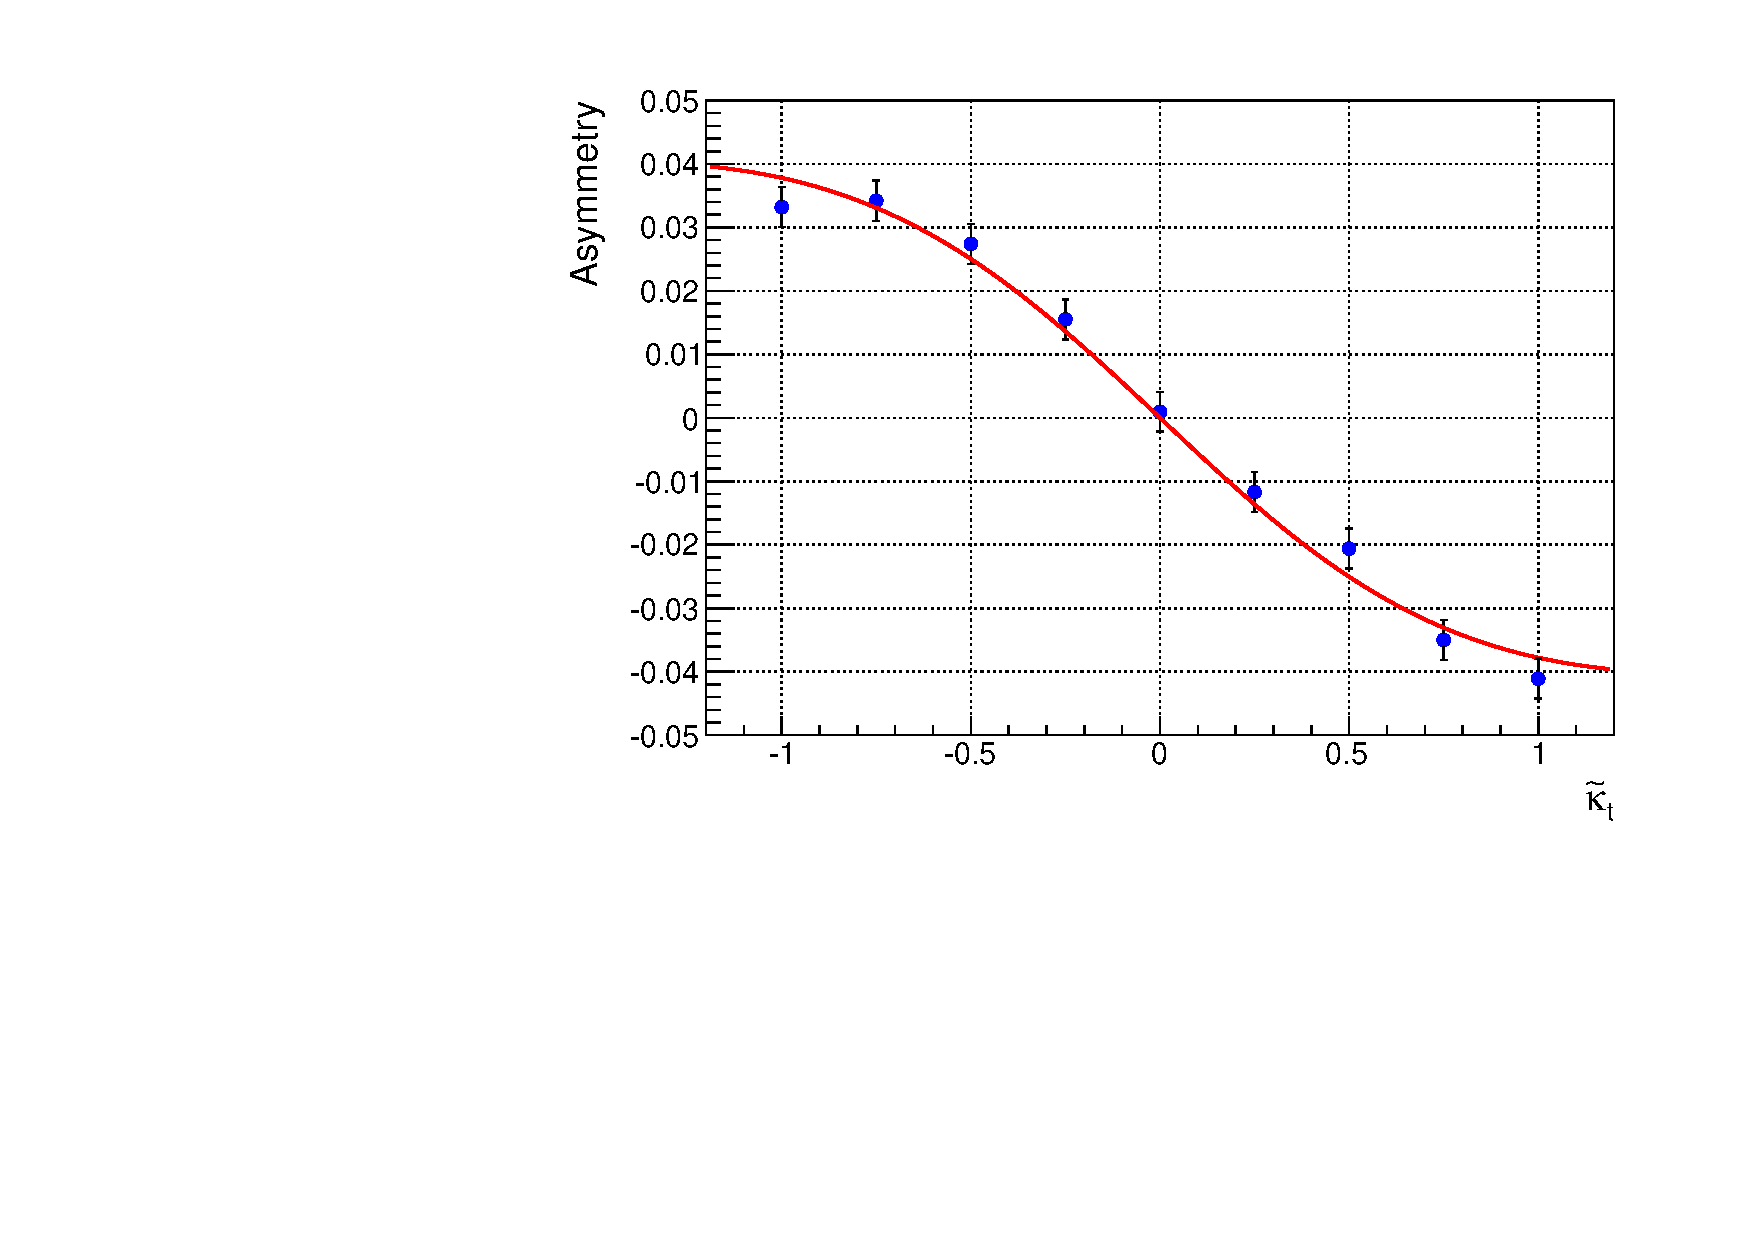
\includegraphics[scale=0.45]{ATP2_nuevo.pdf}} \\
%\hspace*{0.03\textwidth}
\centering
\subfloat{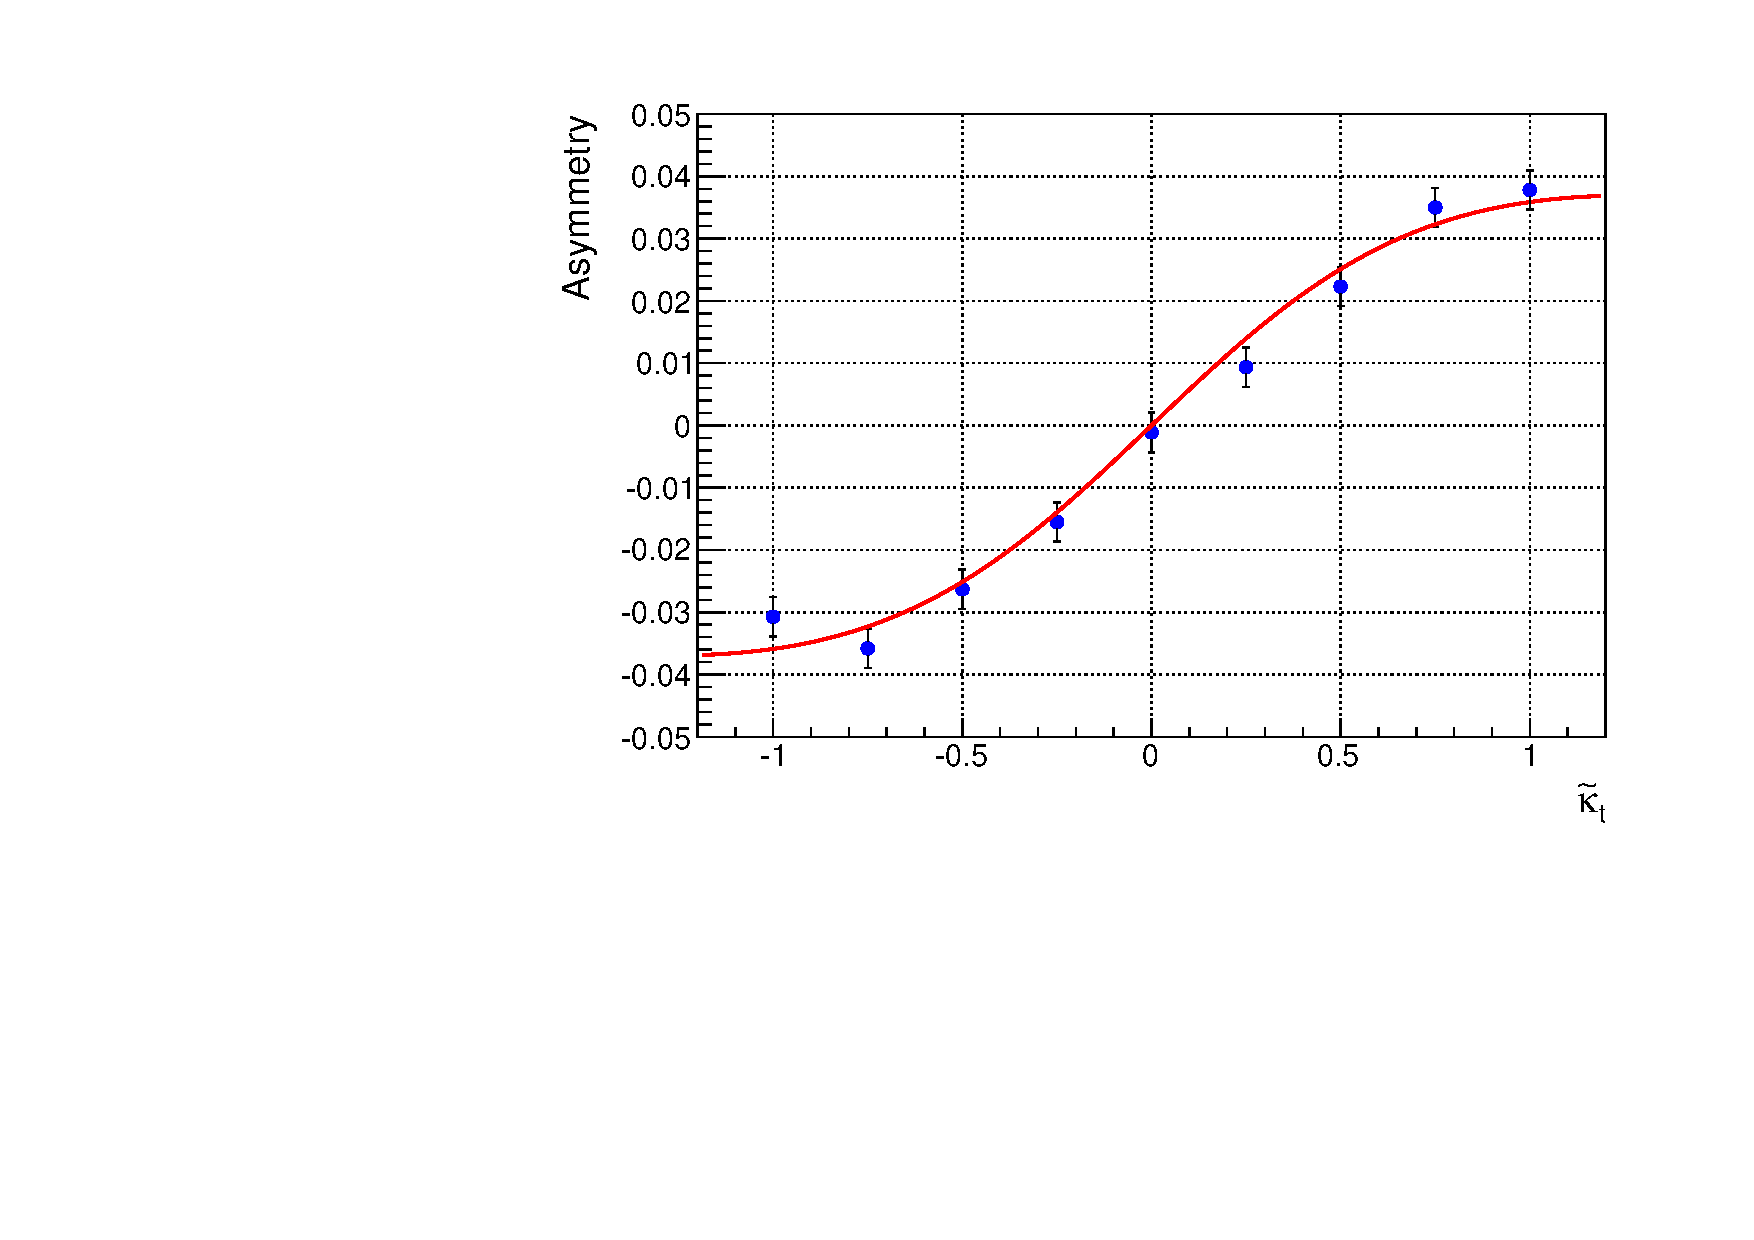
\includegraphics[scale=0.45]{ATP3_nuevo.pdf}}
\caption{Asymmetries for the TPs
  $\epsilon_1=\epsilon(t,\tbar,n_t,n_{\tbar})$ (top-left),
  $\epsilon_2=\epsilon(Q,\tbar,n_t,n_{\tbar})$ (top-right) and
  $\epsilon_3=\epsilon(Q,t,n_t,n_{\tbar})$ (bottom). The points
  represent the values for $\kpt=0,\pm 0.25, \pm 0.5, \pm 0.75,\pm 1$
  and the red solid line is the fitting curve.}
\label{fig3}
\end{figure}
\end{center}
%%%%%%%%%%%%%%%%%%%%%%%%%%%%%%%%%%%%%%%%%%%%
%
%%%%%%%%%%%%%%%%%%%%% FIGURA 4  %%%%%%%%%%%%%%%%%%%%%%%%%%%%
\begin{center}
\vspace*{-4mm}
\begin{figure}[H]
\centering
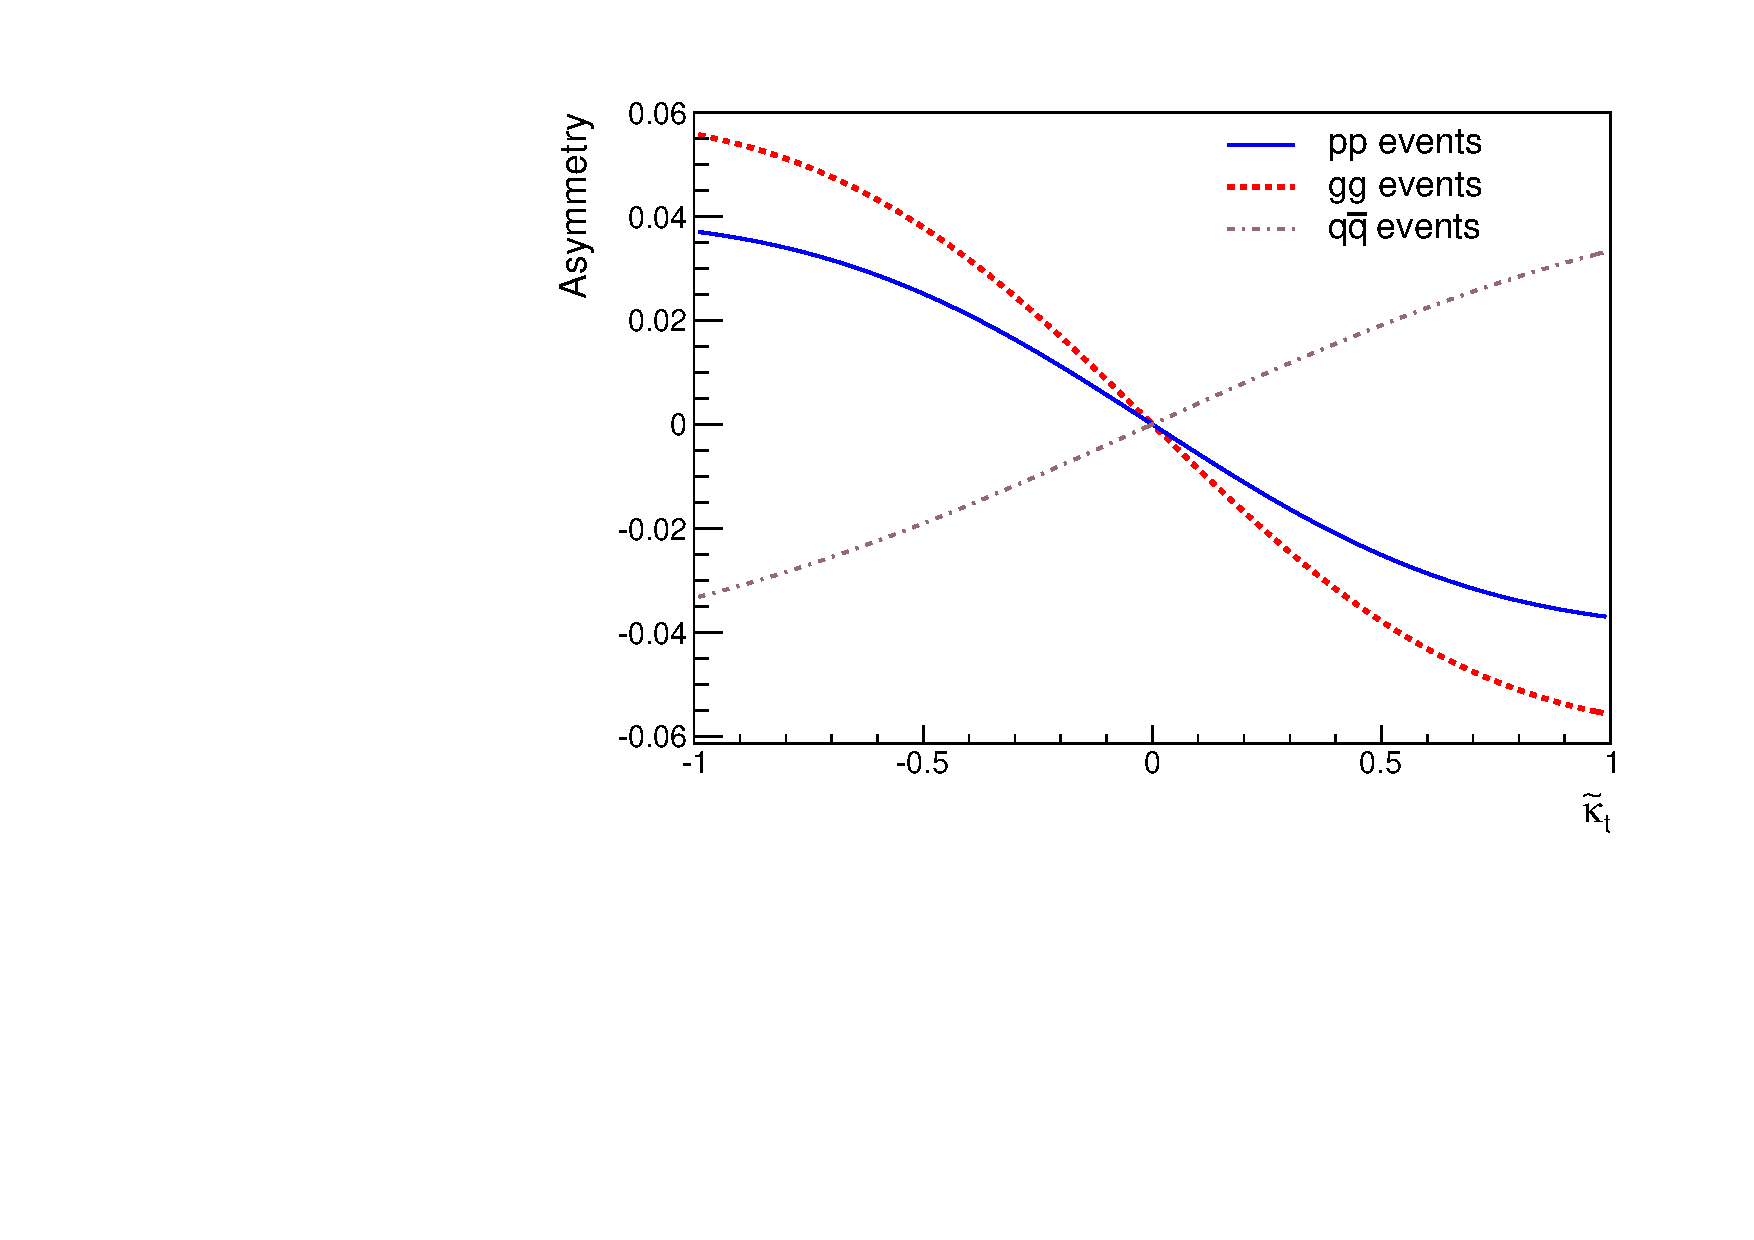
\includegraphics[scale=0.45]{ATP1juntos_nuevo.pdf}
\caption{Asymmetry for the TP
  $\epsilon_1=\epsilon(t,\tbar,n_t,n_{\tbar})$. The dashed line (red)
  corresponds to $gg$-initiated production, the dot-dashed line (grey)
  to $q\qbar$-initiated production and the solid line (blue) to $pp$
  production.}
\label{fig4}
\end{figure}
\end{center}
%%%%%%%%%%%%%%%%%%%%%%%%%%%%%%%%%%%%%%%%%%%%%%%%%%%%%%%%%%%%%
\vspace*{-6mm}

We have also tested various
linear combinations of the TPs $\epsilon_{1,2,3}$ and have found
that the asymmetry is enhanced for the following combination:
%
\beq
\setlength{\abovedisplayskip}{9.5pt}
\setlength{\belowdisplayskip}{9.5pt}
\label{eq24}
\epsilon_4=\epsilon_3-\epsilon_2=\epsilon(Q,t-\tbar,n_t,n_{\tbar}).
\eeq
%
Note that in the $Q$ rest frame, $\epsilon_4=Q^0
(\vec{t}-\vec{\tbar}\,)\cdot(\vec{n}_t\times \vec{n}_{\tbar})$ and the
sign of this TP is determined by the quantity
$(\vec{t}-\vec{\tbar}\,)\cdot(\vec{n}_t\times \vec{n}_{\tbar})$.
{\bf (KK: try to connect previous sentences to something later on\ldots.)}
The
values obtained for the asymmetry associated with this TP are shown in
Table~\ref{table2}. By comparing the results in Tables \ref{table1}
and \ref{table2}, we see that the capability of this
asymmetry to distinguish between the
two $\mathrm{CP}$-mixed hypotheses is increased by at least $3\sigma$.
\vspace{4mm}
\begin{table}[H]
\caption{Asymmetry for the TP $\epsilon_{4}$ for the SM case and the
  two $\mathrm{CP}$-mixed cases defined by $\kp=1,\kpt=\pm 1$. The
  values are obtained by using $10^5$ simulated events.}
\label{table2}
\begin{center}
\begin{tabular}{|C{1cm}|C{1cm}||C{2cm}|C{2cm}|}
%\begin{tabular}{|c|r||r|c||r|c||r|c|}
\hhline{|====|}
%\hhline{|--------|}
$\kappa_t$&$\tilde{\kappa}_t$~~&$\mathcal{A}(\epsilon_4)$~~&$\mathcal{A}(\epsilon_4)/\sigma_{\mathcal{A}}$ \\ 
\hhline{|====|} 
%\hhline{|--------|}
$1$ & $-1$~~~ & $-0.0371$~~~ & $-12$~~~ \\[0.6mm]
\hline
$1$ & $0$ & $0.0004$~ & $0.1$ \\[0.6mm]
\hline
$1$ & $1$ & $0.0461$~ & $14\,$ \\[0.6mm]
\hhline{|====|}
%\hhline{|--------|}
\end{tabular}
\end{center} 
\end{table}
\par Finally, it is worth noting that the asymmetries
described in this subsection are not useful for
discriminating between the SM hypothesis ($\kp=1,\kpt=0$) and the pure
pseudoscalar hypothesis ($\kp=0,\kpt=1$).  Since
the numerators of the 
asymmetries are all linear in both
$\kp$ and $\kpt$, they are expected to vanish in these cases. However, we
will show in the next subsection
that there exist angular distributions
derived from the TPs that are actually suitable for distinguishing between these
two hyphotheses.
%%%%%%%%%%%%%%%%%%%%%%%%%%%%%%%%%%%%%%%%%%%%%%%%%
\subsection{Angular Distributions}
\label{sec3.2}

Given a certain TP, it is possible to define associated angular
distributions that are sensitive to the pseudoscalar coupling
$\kpt$. In order to clarify this, let us first consider the TP
$\epsilon(t,\tbar,n_t,n_{\tbar})$. This TP can be written as
$\epsilon(t+\tbar,\tbar,n_t,n_{\tbar})$, so that in the reference frame
defined by $\vec{t}+\vec{\tbar} =0$ and $\vec{\tbar}\parallel \hat{z}$
we have
%
\beq
\label{eq25}
\epsilon(t+\tbar,\tbar,n_t,n_{\tbar})=M_{t\tbar}\,|\vec{\tbar}|\,(\vec{n}_t\times \vec{n}_{\tbar})_z=M_{t\tbar}\,|\vec{\tbar}||\vec{n}_t||\vec{n}_{\tbar}|\sin\theta_{n_t}\sin\theta_{n_{\tbar}}\sin \Delta \phi(n_t,n_{\tbar}),
\eeq
%
where $M_{t\tbar}$ is the invariant mass of the $t\tbar$ pair, the
angles $\theta_{n_t}$ and $\theta_{n_{\tbar}}$ denote the polar angles
of $\vec{n}_t$ and $\vec{n}_{\tbar}$, respectively, and 
$\Delta\phi(n_t,n_{\tbar})$ is the angular difference between the
projections of $\vec{n}_t$ and $\vec{n}_{\tbar}$ onto the plane
perpendicular to $\vec{\bar{t}}$. If we define the angle
$\Delta\phi(n_t,n_{\tbar})$  to be within the
range $[-\pi,\pi]$, we see from Eq.~(\ref{eq25}) that its sign will
determine the sign of the TP. Thus, the distribution of the
number of events with respect to the angle
$\Delta\phi(n_t,n_{\tbar})$ is related to the asymmetry of the TP,
%
\beq
\label{eq26}
\mathcal{A}(\epsilon)=1-2\frac{N(\epsilon < 0)}{N_T}\,\,\mbox{ and }\,\,\frac{N(\epsilon < 0)}{N_T}=\int^0_{-\pi}\frac{1}{N_T}\frac{dN}{d\Delta\phi(n_t,n_{\tbar})}\,d\Delta\phi(n_t,n_{\tbar}),
\eeq  
%
where $N_T$ is the total number of events.
{\bf (KK: Have we checked numerically that the above
  expression does indeed hold numerically for the various
  distributions?  It's an exact relation, correct?)}
Moreover, for a certain TP
one can derive different angular distributions by considering
different reference frames, although all of these will satisfy
Eq.~(\ref{eq26}) (note that $\mathcal{A}(\epsilon)$
is Lorentz invariant). Recalling the various TPs considered
in Sec.~\ref{sec2}, we examine the following angular distributions.
\begin{enumerate}
\item {\boldmath $\epsilon_1 = \TPa$.}  To probe $\epsilon_1$, we construct
  the distribution
  $d\sigma/d\Delta\phi_1(n_t,n_{\tbar})$ in the rest frame of $t\tbar$,
  taking $\vec{\tbar}$ to define the $z$-axis. The angle
  $\Delta\phi_1(n_t,n_{\tbar})$ is the angular difference between the
  projection of the spin vectors in the plane perpendicular to
  $\vec{\tbar}$.
\item {\boldmath $\epsilon_2 = \TPb$.}  In this case, we
  define the distribution
  $d\sigma/d\Delta\phi_2(n_t,n_{\tbar})$ in the rest frame of $Q$, taking
  $\vec{\tbar}$ to define the $z$-axis. The angle
  $\Delta\phi_2(n_t,n_{\tbar})$ is the angular difference between the
  projection of the spin vectors in the plane perpendicular to
  $\vec{\tbar}$.
\item {\boldmath $\epsilon_3 = \TPc$.}  The distribution
  $d\sigma/d\Delta\phi_3(n_t,n_{\tbar})$ is also defined
  in the rest frame of $Q$, but this time taking
  $\vec{t}$ to be along the $z$-axis. The angle $\Delta\phi_3(n_t,n_{\tbar})$
  is the angular difference between the projection of the spin vectors
  in the plane perpendicular to $\vec{t}$.
\end{enumerate}
\par
%
Figure~\ref{fig5} shows the normalized distributions obtained
for the first case listed above.
Four scenarios are considered, corresponding to the SM
($\kp= 1$ and $\kpt=0$), two cases in which the Higgs boson
has mixed $\mathrm{CP}$ couplings ($\kp= 1$ and $\kpt=\pm 1$)
and a case in which the Higgs boson is purely 
$\mathrm{CP}$-odd ($\kp= 0,\kpt=1$). Figure~\ref{fig6} shows
the analogous distributions for $\epsilon_2$. The distributions
corresponding to $\epsilon_3$ are similar to those of $\epsilon_2$,
except that the ``shifts'' are in the opposite directions for
the two mixed-$\mathrm{CP}$ cases.  Given the similarities of the
plots we do not include them here.  {\bf (KK: did I reword this correctly?)}
%%%%%%%%%%%%%%%%%%%%%%%%% FIGURA 5 %%%%%%%%%%%%%%%%%%%%%%%%%
%%%% ruta turin facultad: /home/nico/Documentos/ttbarH/Material_final/ todas las figs para abajo
\begin{center}
\vspace*{1.4mm}
\begin{figure}[H]
%\centering
\hspace*{-0.52cm}
\subfloat{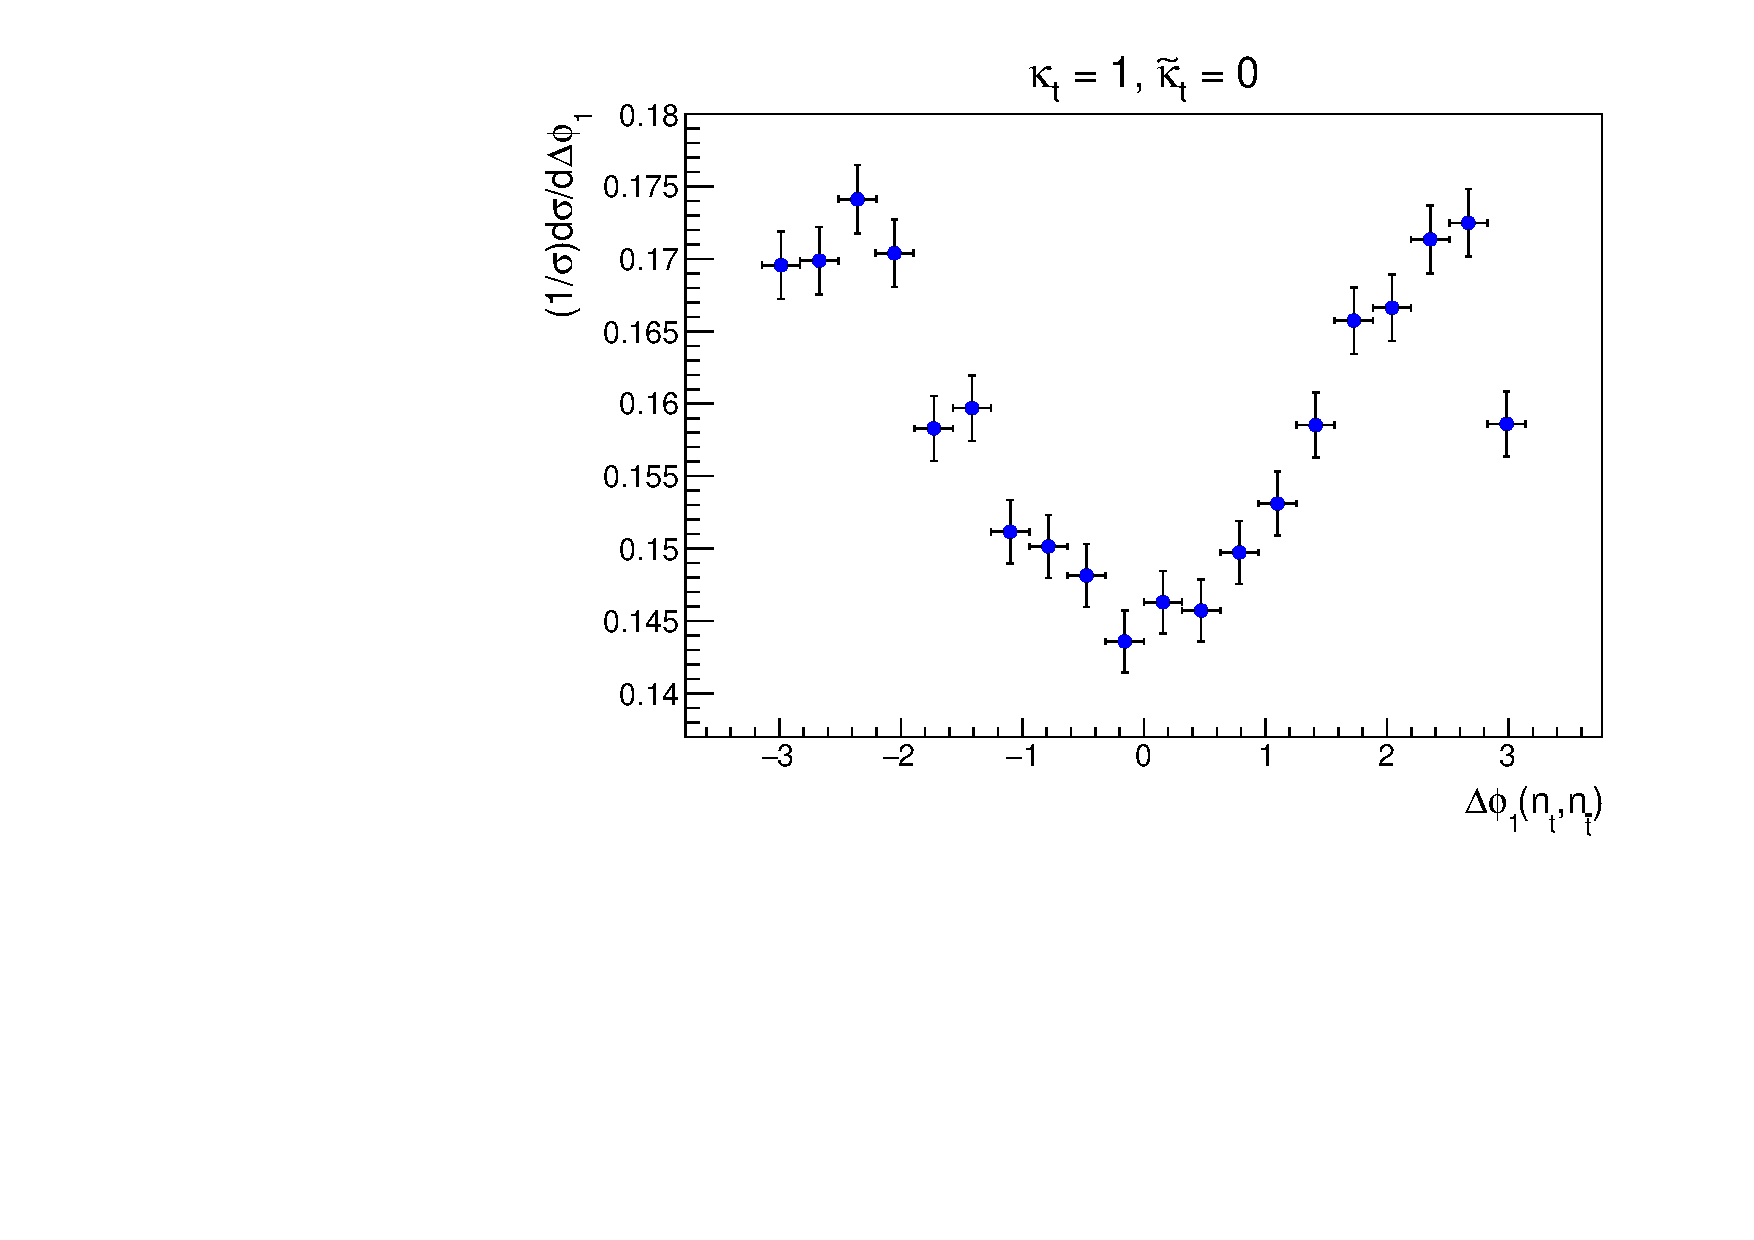
\includegraphics[scale=0.45]{TP1_10_nuevo.pdf}}
\hspace*{-0.006\textwidth}
\subfloat{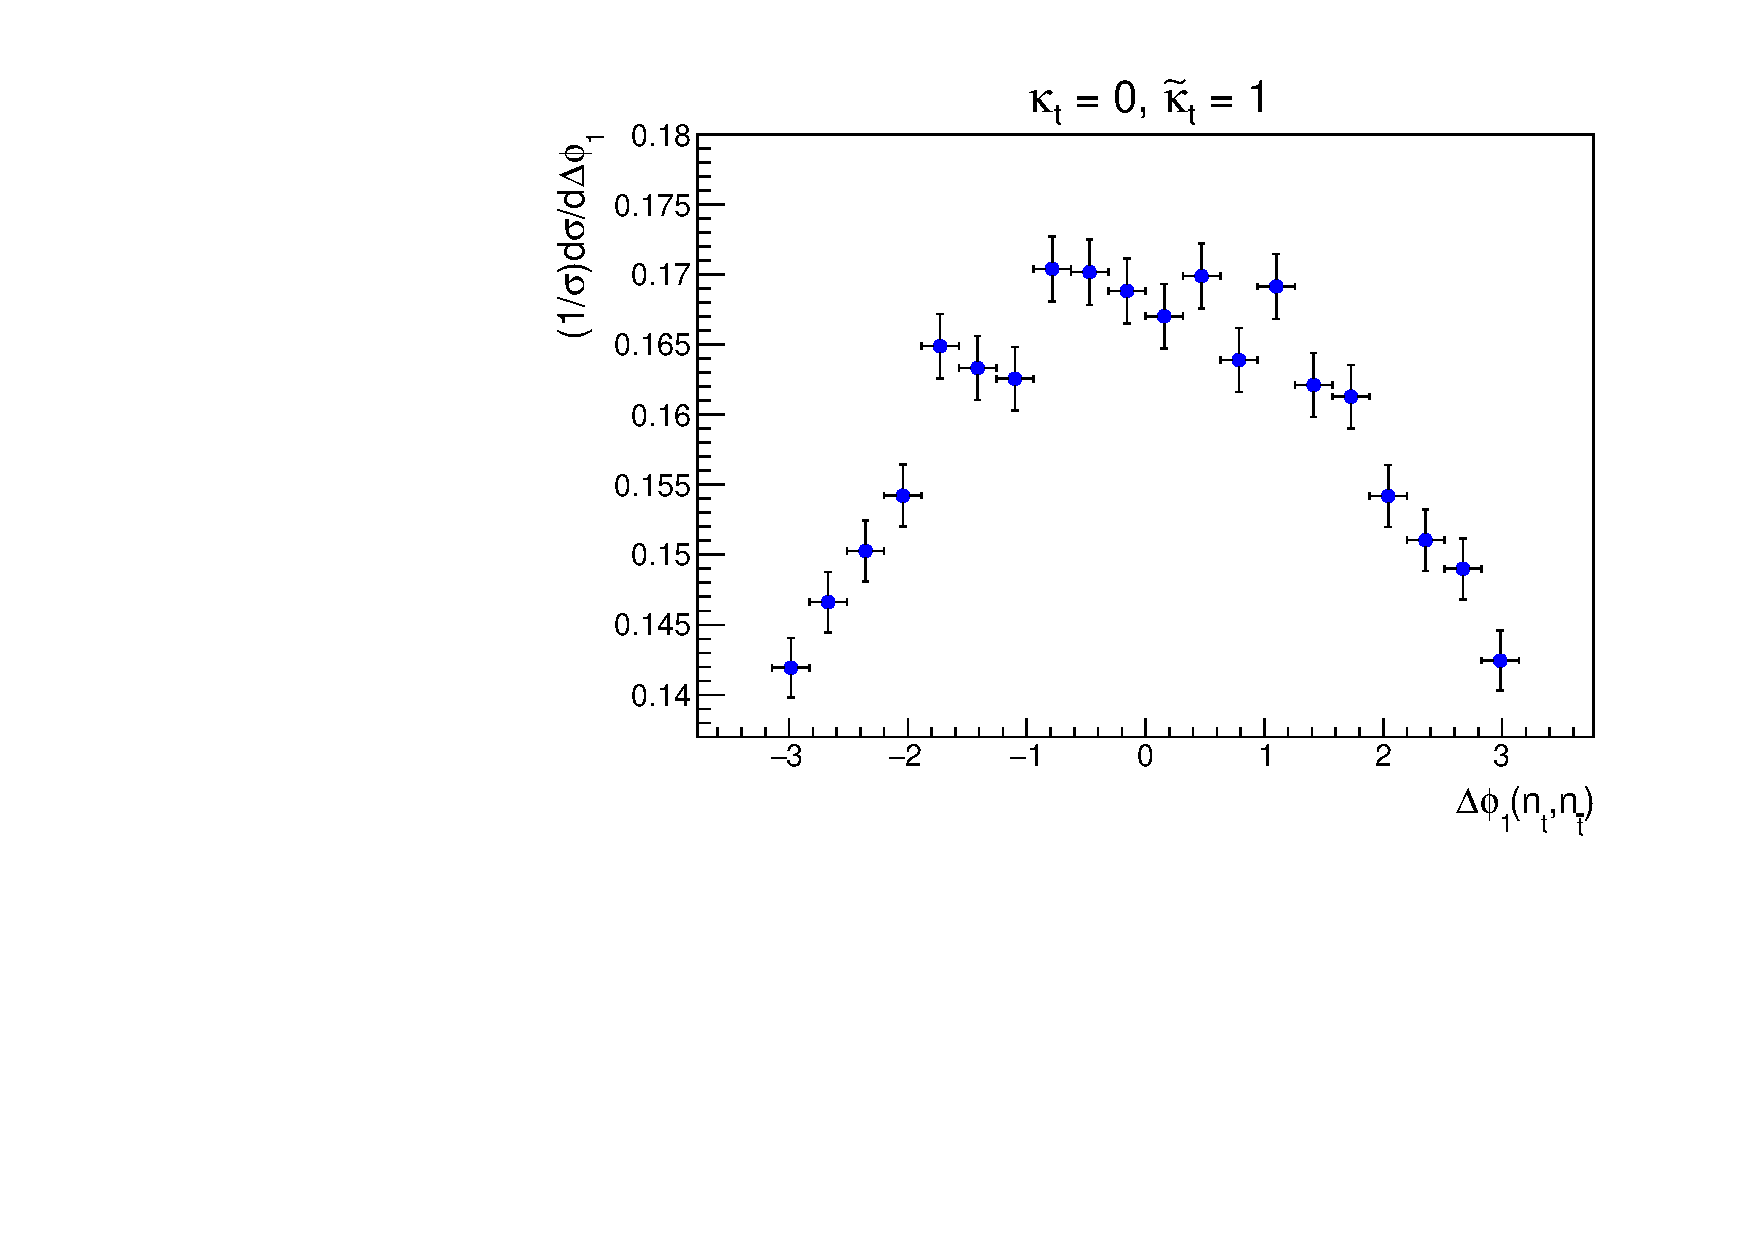
\includegraphics[scale=0.45]{TP1_01_nuevo.pdf}} \\
\hspace*{-0.45cm}
%\hspace*{0.03\textwidth}
\subfloat{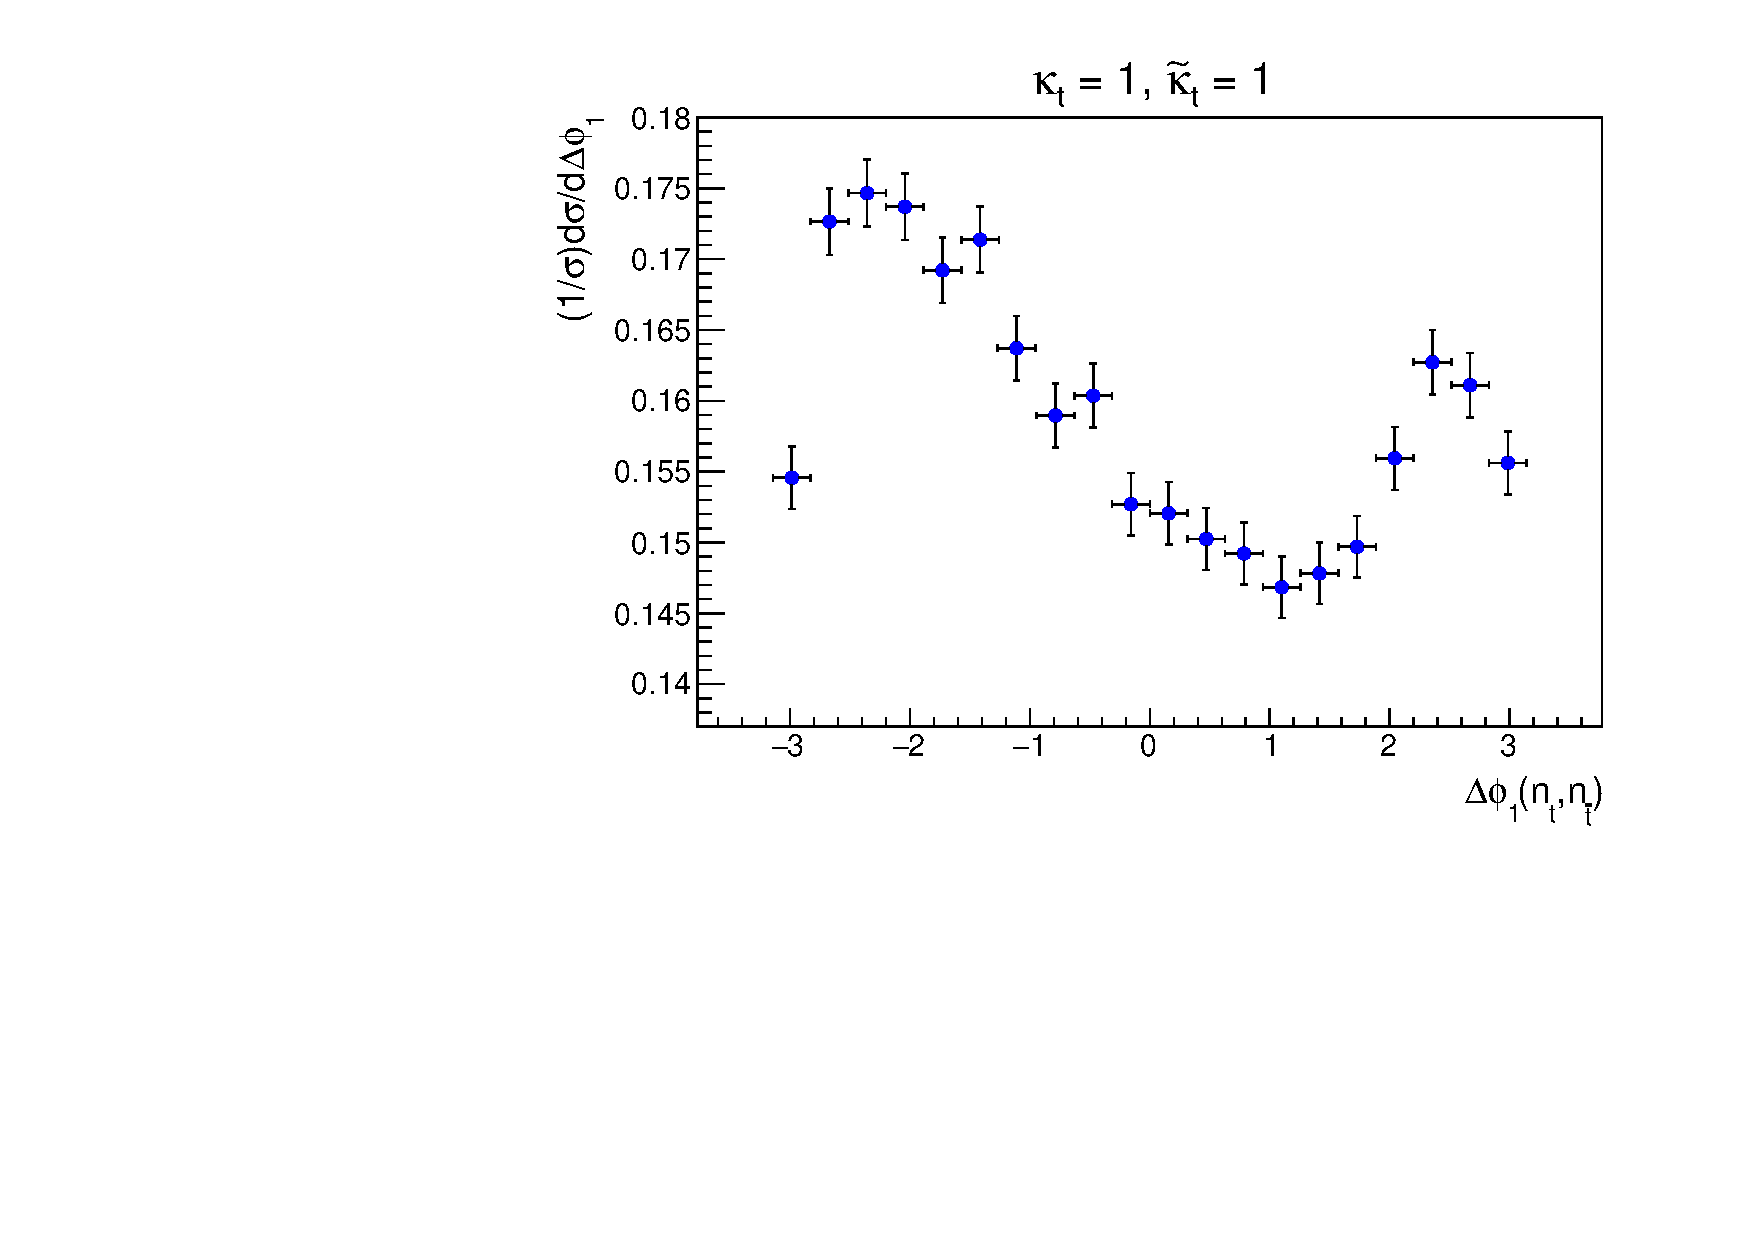
\includegraphics[scale=0.45]{TP1_11_nuevo.pdf}}
\hspace*{-0.006\textwidth}
\subfloat{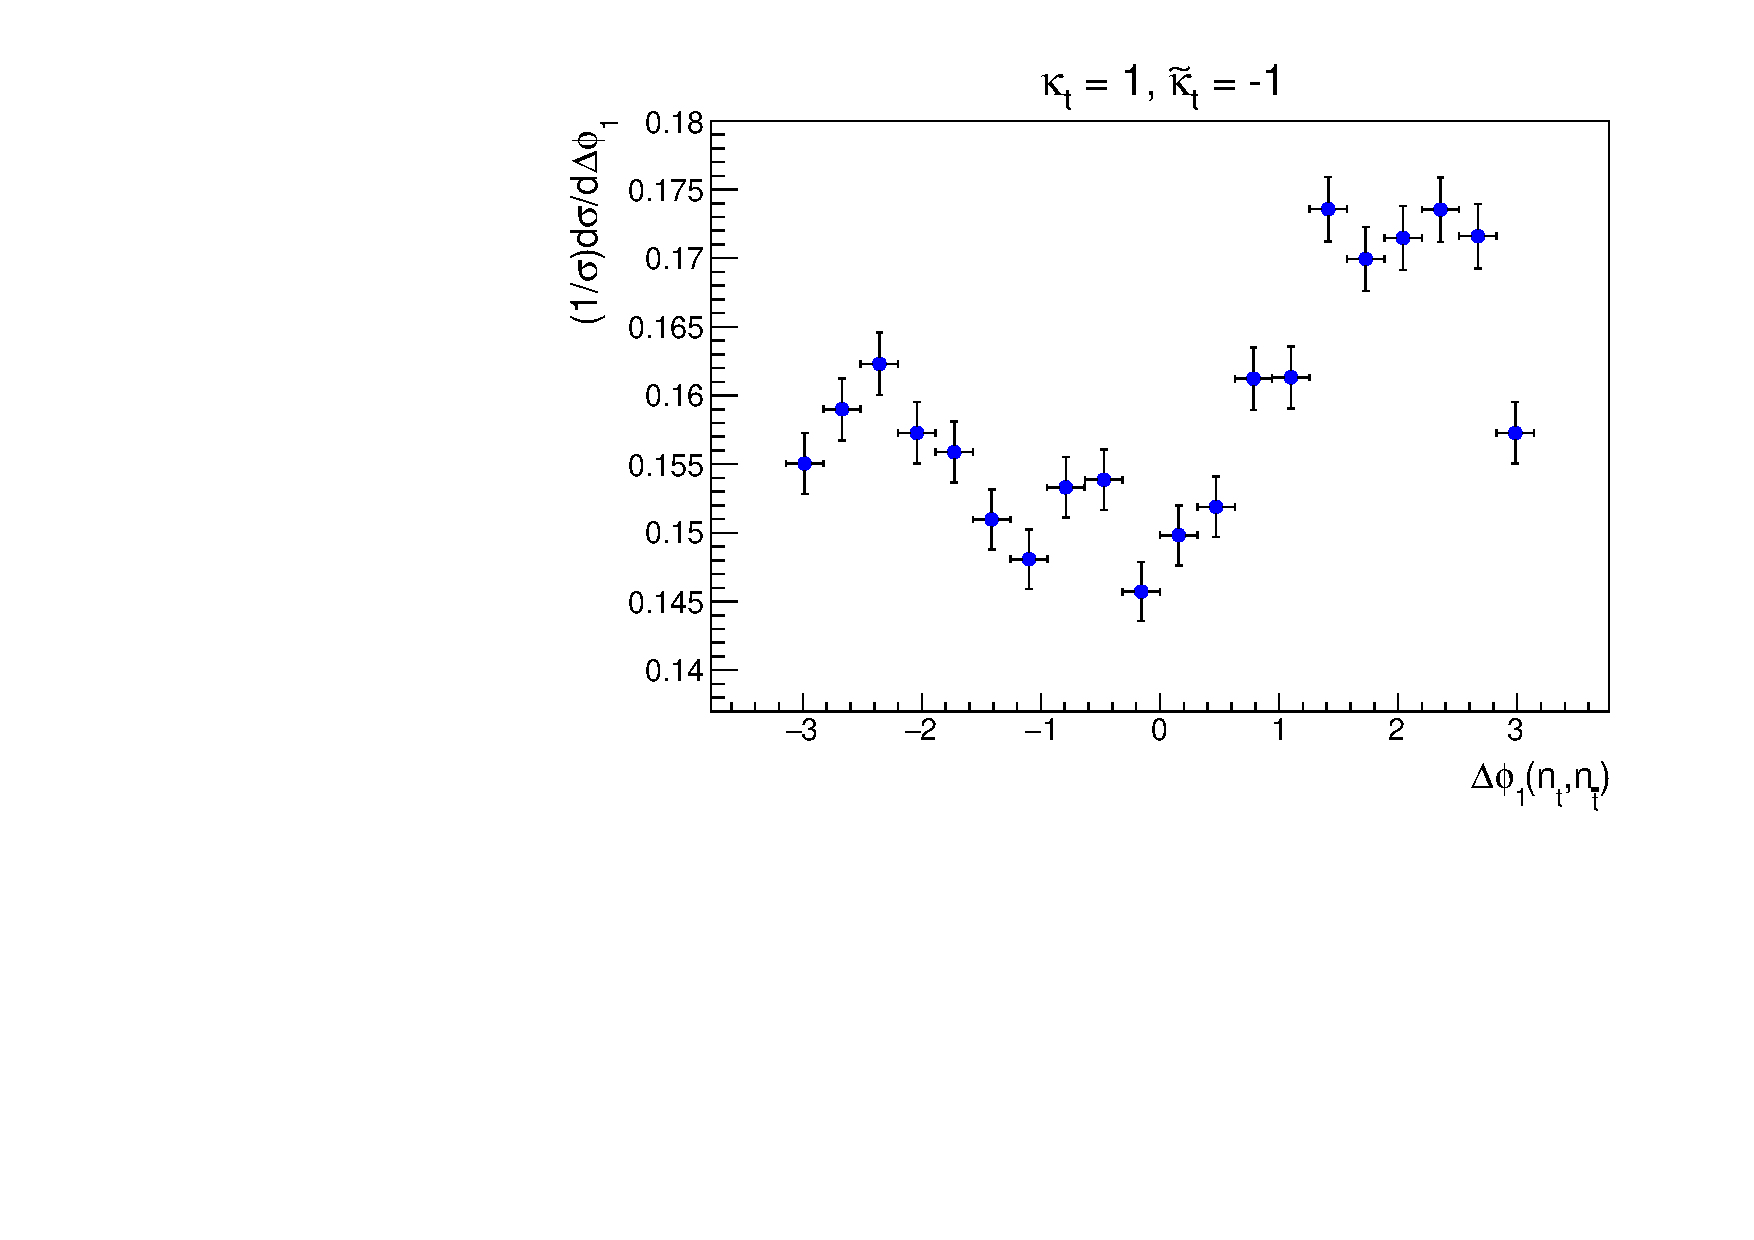
\includegraphics[scale=0.45]{TP1_1-1_nuevo.pdf}}
\caption{Angular distributions associated with the TP
  $\epsilon_1 = \epsilon(t,\tbar,n_t,n_{\tbar})$ for various values of
  $\kp$ and $\kpt$. The error bars correspond to the statistical
  uncertainties.}
\label{fig5}
\end{figure}
\end{center}
%%%%%%%%%%%%%%%%%%%%%%%%% FIGURA 6 %%%%%%%%%%%%%%%%%%%%%%%%%
\begin{center}
%\vspace*{-4mm}
\begin{figure}[H]
%\centering
\hspace*{-0.52cm}
\subfloat{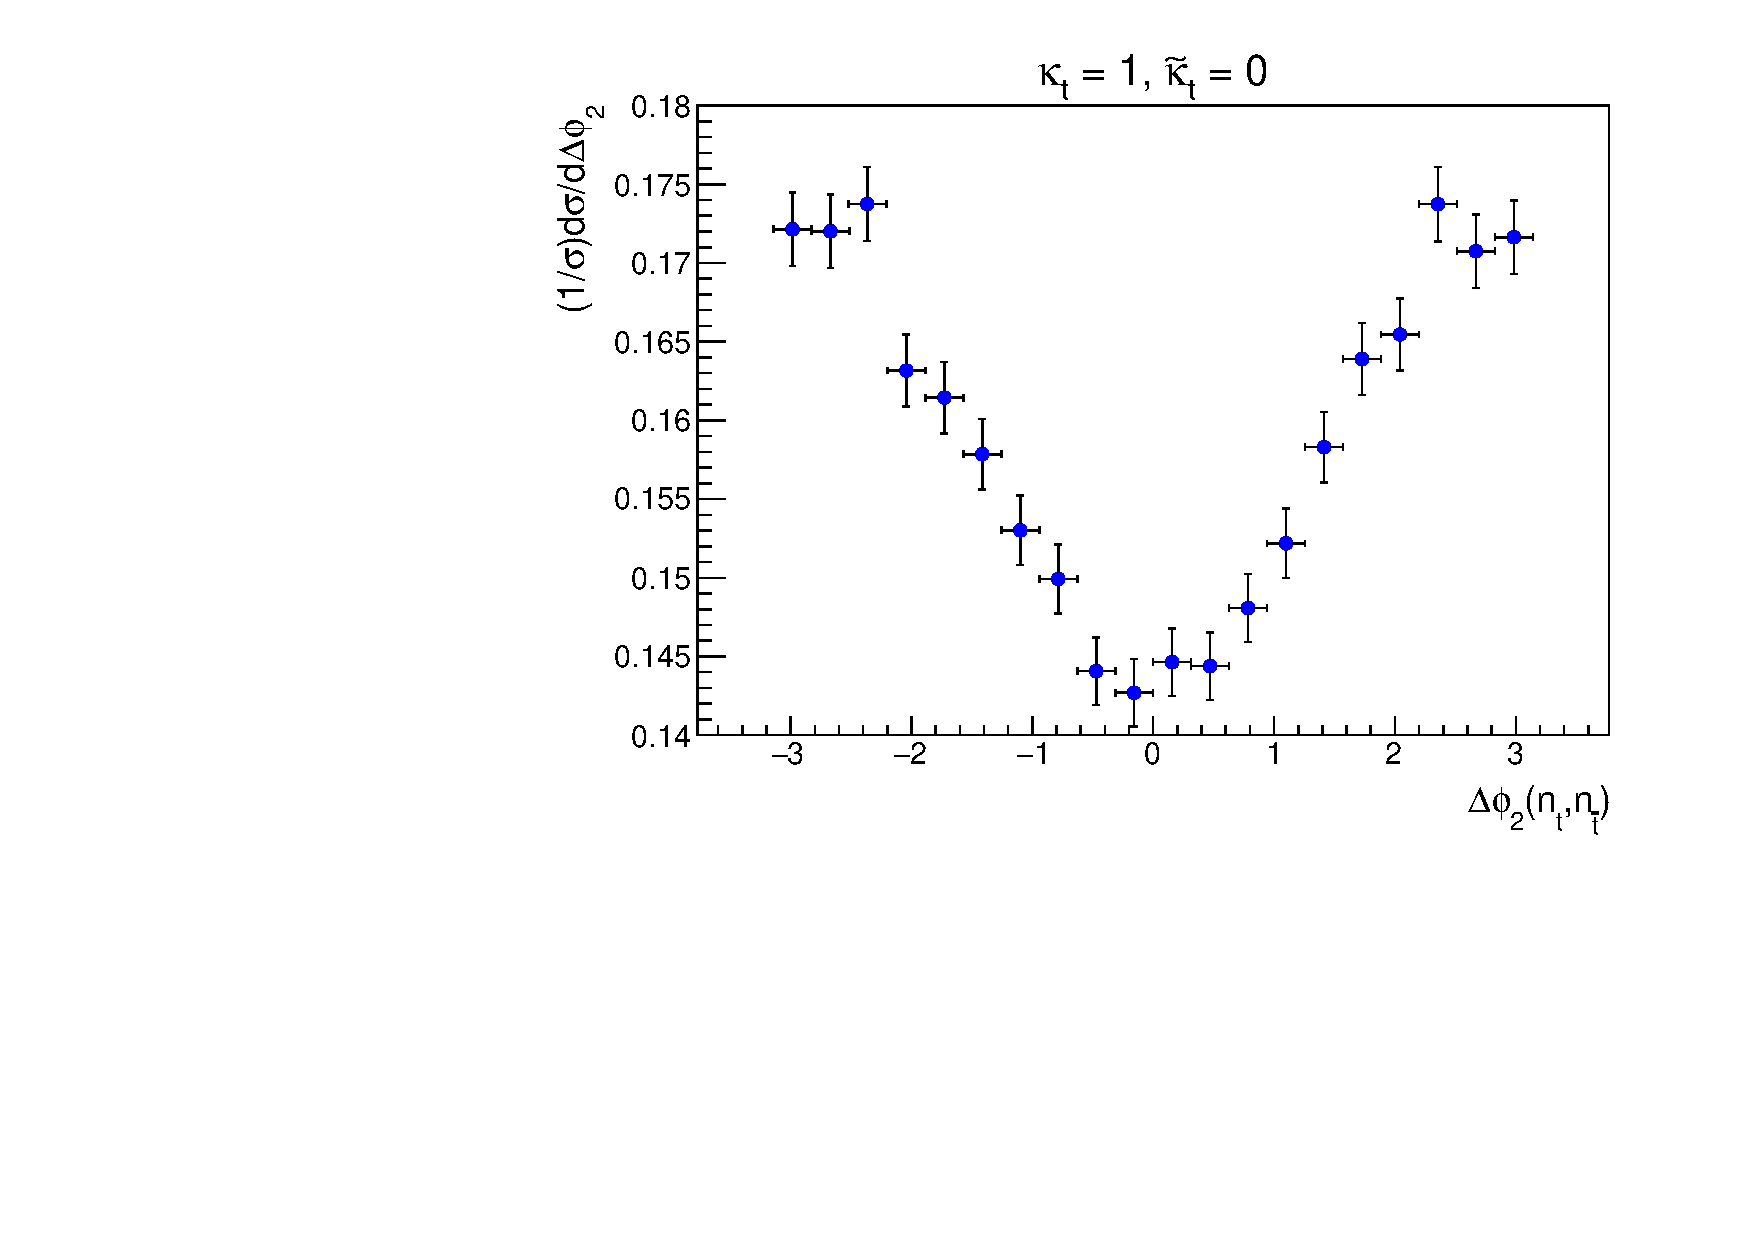
\includegraphics[scale=0.45]{TP2_10_nuevo.pdf}}
\hspace*{-0.006\textwidth}
\subfloat{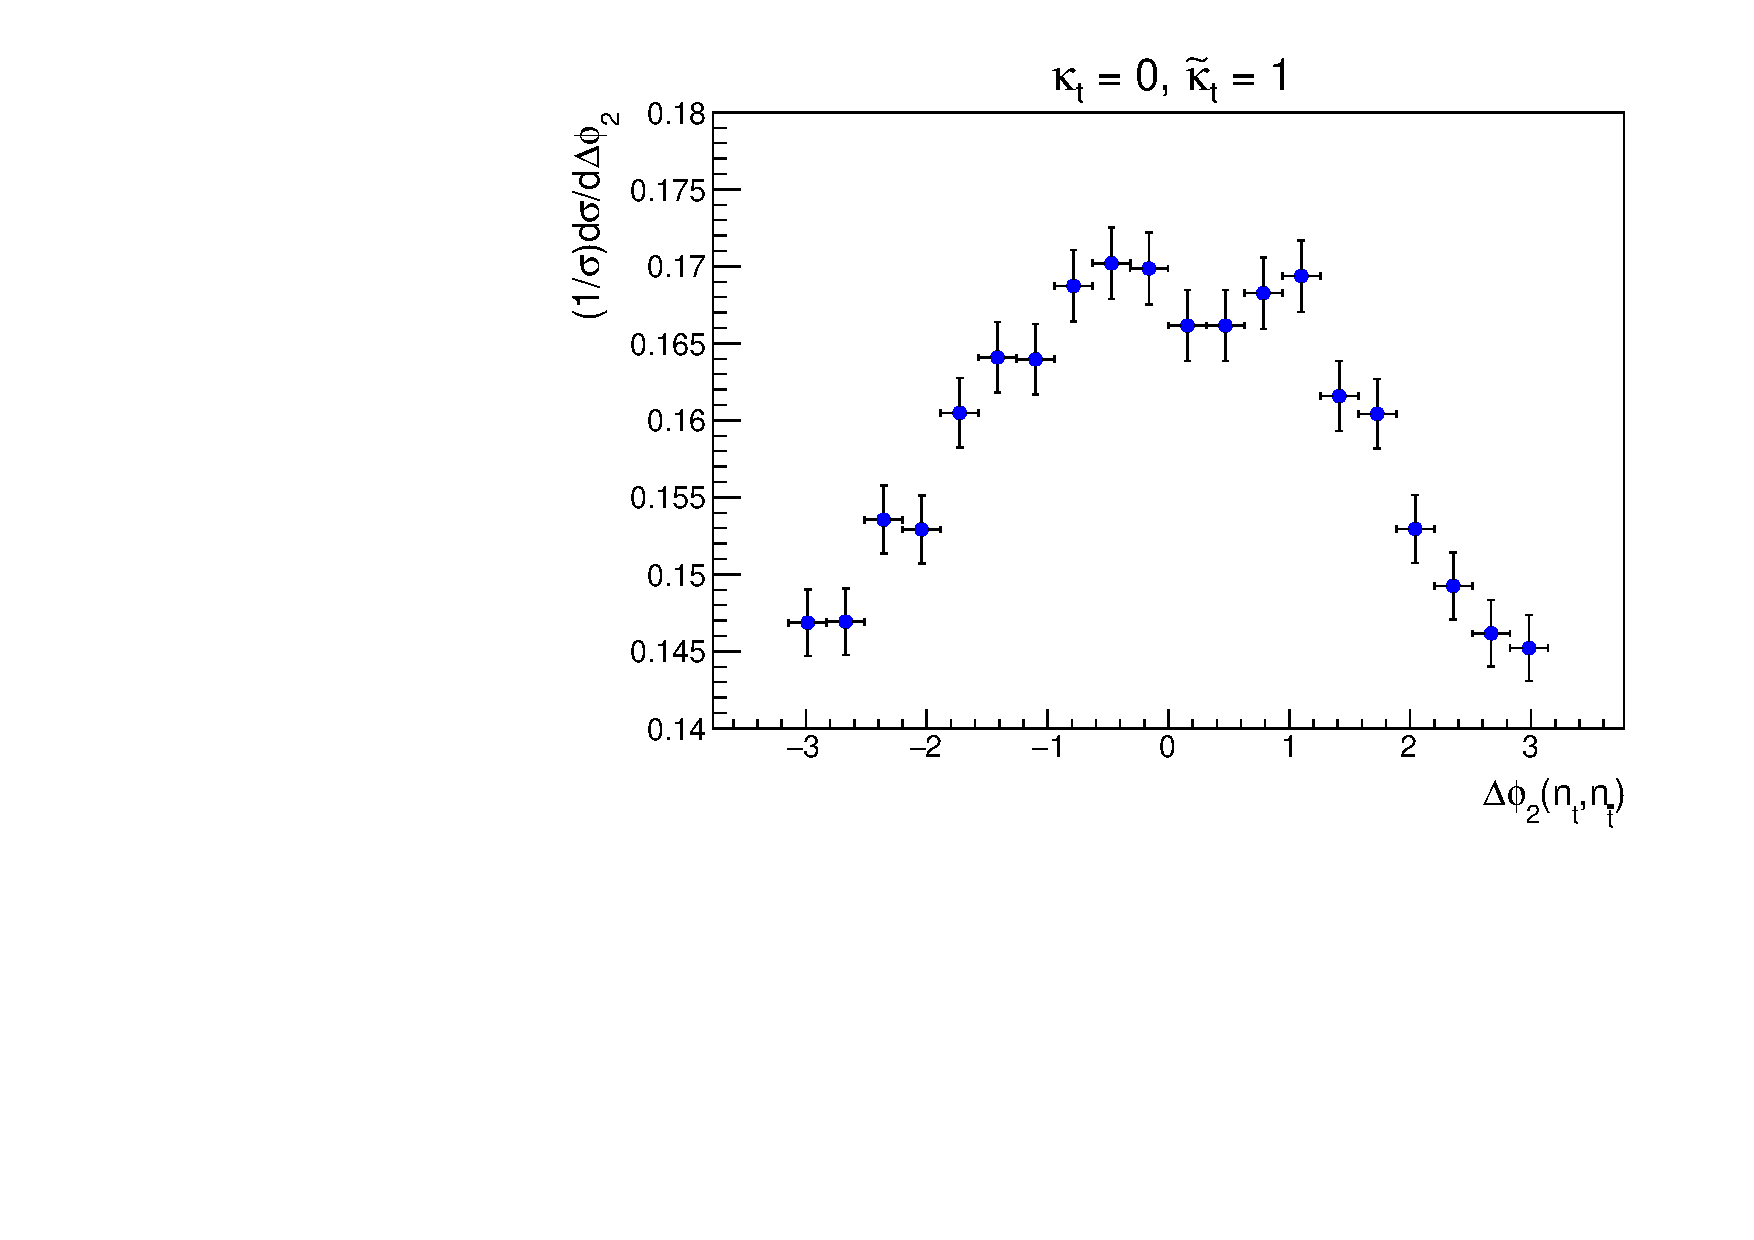
\includegraphics[scale=0.45]{TP2_01_nuevo.pdf}} \\
\hspace*{-0.45cm}
%\hspace*{0.03\textwidth}
\subfloat{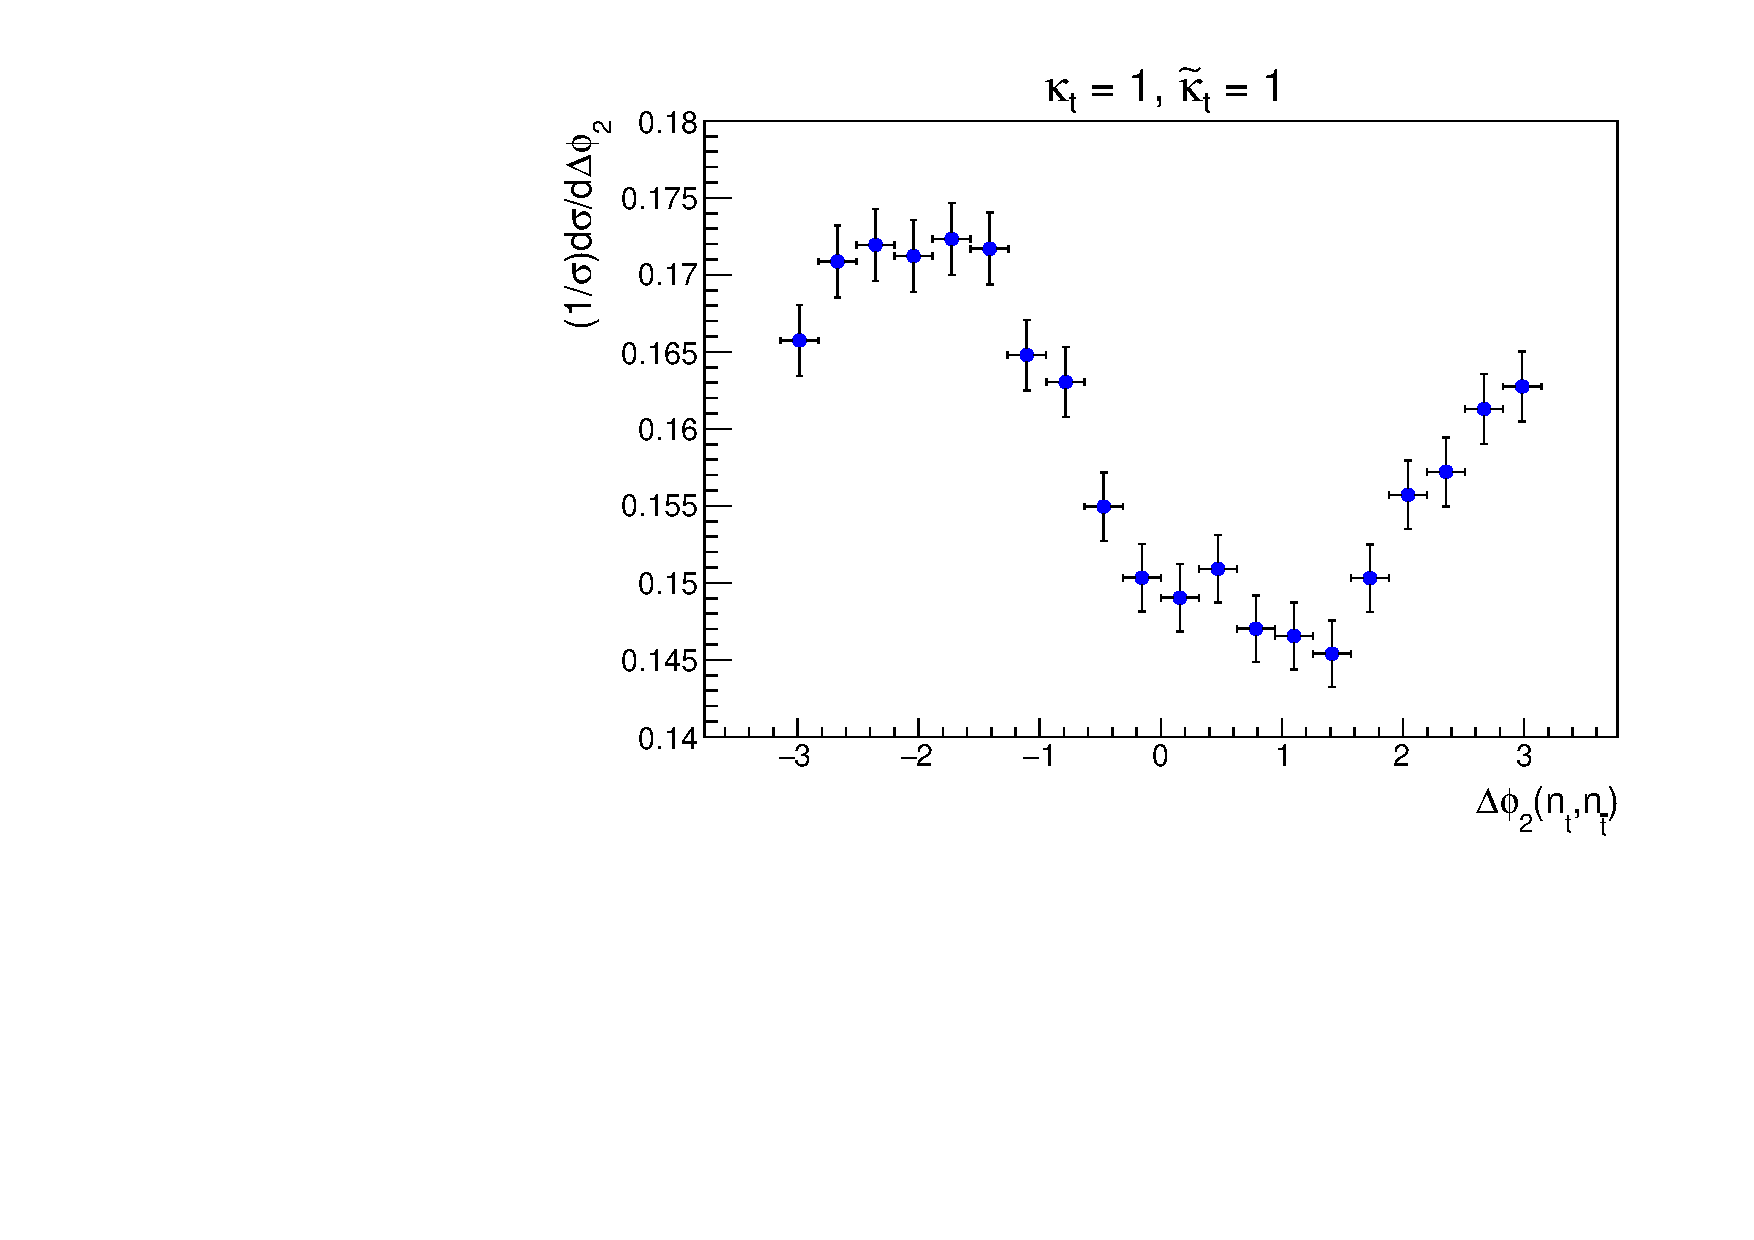
\includegraphics[scale=0.45]{TP2_11_nuevo.pdf}}
\hspace*{-0.006\textwidth}
\subfloat{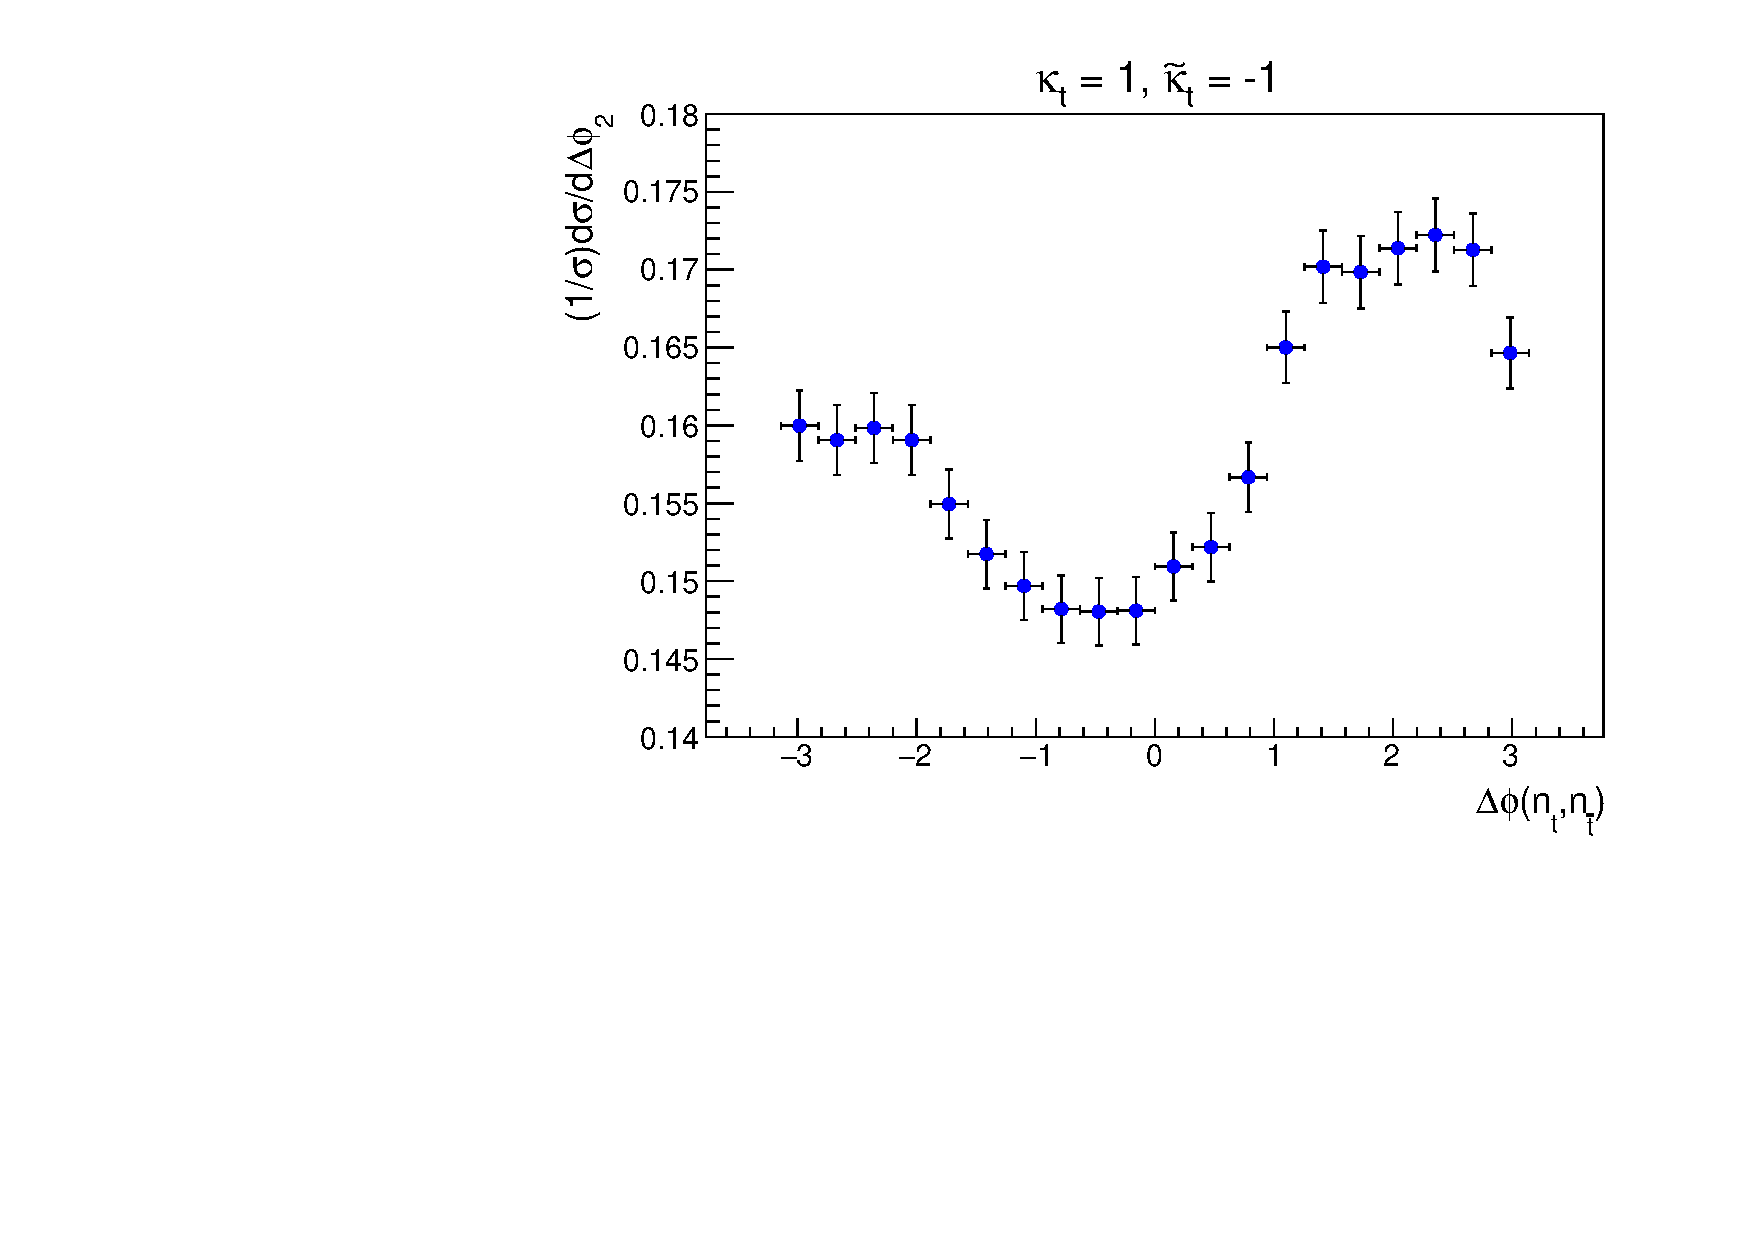
\includegraphics[scale=0.45]{TP2_1-1_nuevo.pdf}}
\caption{Angular distributions associated with the TP $\epsilon_2 = \TPb$ for
  various values of $\kp$ and $\kpt$. The error bars indicate the statistical
  uncertainties.}
\label{fig6}
\end{figure}
\end{center}
\par As can be seen from Figs.~\ref{fig5} and \ref{fig6}, the
peaks of the 
distributions are shifted to the left or the right of the origin
in the mixed-$\mathrm{CP}$
cases ($\kp =1$ and $\kpt=\pm 1$).
The magnitude of the shift appears to be approximately the
same in both cases, but with
opposite sign for $\kp=\kpt=1$ and $\kp=-\kpt=1$, thus allowing
one to distinguish
the sign of the pseudoscalar coupling. The observed dependence
on the sign of $\kpt$ in these cases
is consistent with the fact that the numerator of $\mathcal{A}(\epsilon)$
is linear in $\kpt$ [see Eq.~(\ref{eq26})]
and that the quantity $N(\epsilon < 0)/N_T$ is related
to the angular distribution according to Eq.~(\ref{eq26}). The angular
distributions for the SM case ($\kp =1$ and $\kpt=0$) and
the pure pseudoscalar case ($\kp =0$ and $\kpt= 1$) are
visibly different from each other and from the mixed-$\mathrm{CP}$
scenarios. Comparing the SM and purely pseudoscalar cases,
we note that while the angular distributions for the former case
exhibit a minimum at $\Delta\phi_{1,2}(n_t,n_{\tbar})=0$, those
for the latter case exhibit a peak at this location.
Thus, these two scenarios can be distinguished from each other
via these angular distributions.  This is to be contrasted
with the situation for the asymmetries $\mathcal{A}(\epsilon)$, which vanish
in both cases.  In order to quantify the mentioned shifts, we have fitted
the simulated distributions with the following function proposed in
\cite{Ellis},
%
\beq
\label{eq27}
\frac{1}{\sigma}\frac{d\sigma}{d\Delta\phi_i(n_t,n_{\tbar})}=a_0 + a_1\cos(\Delta\phi_i(n_t,n_{\tbar})+\delta),\qquad\, i=1,2,3.
\eeq
%
To the extent that this equation is exact we note that
Eq.~(\ref{eq29}) gives $\mathcal{A}(\epsilon_i)=4a_1 \sin\delta$. With
this fitting function, we obtain phase shifts approximately between
$0.9$ and $1$ ($-1$ and $-0.9$) for $\kp=\kpt=1$ ($\kp=-\kpt=1$) both
for $\epsilon_1$ and $\epsilon_2$. However, the quality of the fits is
not good enough, being worse in the case of the $\epsilon_1$
distributions for which $\chi^2/\mathrm{d.o.f}$ is in the range
$1.69$-$3.86$, in contrast to the range $0.53$-$1.16$ obtained for
$\epsilon_2$. The main impact on the deviation from the functional
form proposed in Eq.~(\ref{eq27}) appears to be caused by the $\Delta
R_{ll}$ cut we have imposed. In fact, when this cut is turned off the
above ranges for $\chi^2/\mathrm{d.o.f}$ modify to $0.75$-$1.14$ and
$0.44$-$1.07$ for the $\epsilon_1$ and $\epsilon_2$ distributions
respectively. In Tables \ref{table3} and \ref{table4} we list the
results of the fits obtained when the $\Delta R_{\ell\ell}$ cut is
relaxed. The results for the TP $\epsilon_3$ are pretty similar to
those for $\epsilon_2$ but with opposite sign in the phase shifts of
the $\mathrm{CP}$-mixed hypotheses and hence we do not include them
here. In addition, we show in Fig.~\ref{fig7} the angular
distributions along with the fit curves for both $\mathrm{CP}$-mixed
cases when no cut is imposed in $\Delta R_{\ell\ell}$.
\renewcommand{\arraystretch}{1.2}
\begin{table}[H]
\caption{Fit results for the angular distribution $d\sigma/(\sigma
  d\Delta\phi_1(n_t,n_{\tbar}))$ related to the TP
  $\epsilon_1=\epsilon(t,\tbar,n_t,n_{\tbar})$ when the $\Delta
  R_{\ell\ell}$ is turned off. Note that the parameter $a_1$ change
  its sign for $\kp=0,\kp=1$.}
\label{table3}
\begin{center}
\begin{tabular}{|C{1cm}|C{1cm}||C{3cm}|C{3cm}|C{3cm}|}
%\begin{tabular}{|c|r||r|c||r|c||r|c|}
\hhline{|=====|}
%\hhline{|--------|}
$\kappa_t$&$\tilde{\kappa}_t$~~&$a_0$~~&$a_1$& $\delta$~~ \\ 
\hhline{|=====|} 
%\hhline{|--------|}
$1$ & $-1$~~~ & $0.1592 \pm 0.0006$ & $-0.0139 \pm 0.0008$ & $0.81 \pm 0.07$ \\[0.6mm]
\hline
$1$ & $0$ & $0.1595 \pm 0.0006$ & $-0.0181 \pm 0.0008$ & $0.002 \pm 0.06\,\,$ \\[0.6mm]
\hline
$1$ & $1$ & $0.1591 \pm 0.0006$ & $-0.0131 \pm 0.0008 $ & $\,-0.82 \pm 0.07\quad$  \\[0.6mm]
\hline
$0$ & $1$ & $0.1591 \pm 0.0006$ & ~~$\,0.0102 \pm 0.0008$ & $0.11 \pm 0.08$ \\
\hhline{|=====|}
%\hhline{|--------|}
\end{tabular}
\end{center} 
\end{table}
%%%%%%%%%%%%%%%%%%%%%%%%%%%%%%%%%%%%%%%%%%%%%%%%%%%%%
\begin{table}[H]
\caption{Fit results for the angular distribution $d\sigma/(\sigma
  d\Delta\phi_2(n_t,n_{\tbar}))$ related to the TP
  $\epsilon_2=\epsilon(Q,\tbar,n_t,n_{\tbar})$ when the $\Delta
  R_{\ell\ell}$ is turned off. Note that the parameter $a_1$ change
  its sign for $\kp=0,\kp=1$.}
\label{table4}
\begin{center}
\begin{tabular}{|C{1cm}|C{1cm}||C{3cm}|C{3cm}|C{3cm}|}
%\begin{tabular}{|c|r||r|c||r|c||r|c|}
\hhline{|=====|}
%\hhline{|--------|}
$\kappa_t$&$\tilde{\kappa}_t$~~&$a_0$~~&$a_1$& $\delta$~~ \\ 
\hhline{|=====|} 
%\hhline{|--------|}
$1$ & $-1$~~~ & $0.1591 \pm 0.0006$ & $-0.0146 \pm 0.0008$ & $0.73 \pm 0.06$ \\[0.6mm]
\hline
$1$ & $0$ & $0.1594 \pm 0.0007$ & $-0.0190 \pm 0.0008$ & $0.005 \pm 0.06\,\,$ \\[0.6mm]
\hline
$1$ & $1$ & $0.1592 \pm 0.0006$ & $-0.0136 \pm 0.0008 $ & $\,-0.77 \pm 0.07\quad$  \\[0.6mm]
\hline
$0$ & $1$ & $0.1591 \pm 0.0006$ & ~~$\,0.0113 \pm 0.0008$ & $0.09 \pm 0.08$ \\
\hhline{|=====|}
%\hhline{|--------|}
\end{tabular}
\end{center} 
\end{table}
\par From Tables \ref{table3} and \ref{table4} we see that the
parameter $\delta$ is sensitive not only to the modulus of $\kpt$ but
also to its sign, as expected if Eq.~(\ref{eq26}) is taken into
account. The phase shift $\delta$ for the distribution of the angle
$\Delta\phi_1$ appears to exhibit a slightly higher sensitivity than
that obtained from the $\Delta\phi_2$-distribution, albeit both are
still compatible within the statistical uncertainties. However, it is
important to stress that the fits of the $\Delta\phi_2$-distributions
give allways smaller values for $\chi^2/\mathrm{d.o.f}$.
%%%%%%%%%%%%%%%%%%%%%%%%% FIGURA 7 %%%%%%%%%%%%%%%%%%%%%%%%%
\begin{center}
%\vspace*{-4mm}
\begin{figure}[H]
%\centering
\hspace*{-0.52cm}
\subfloat{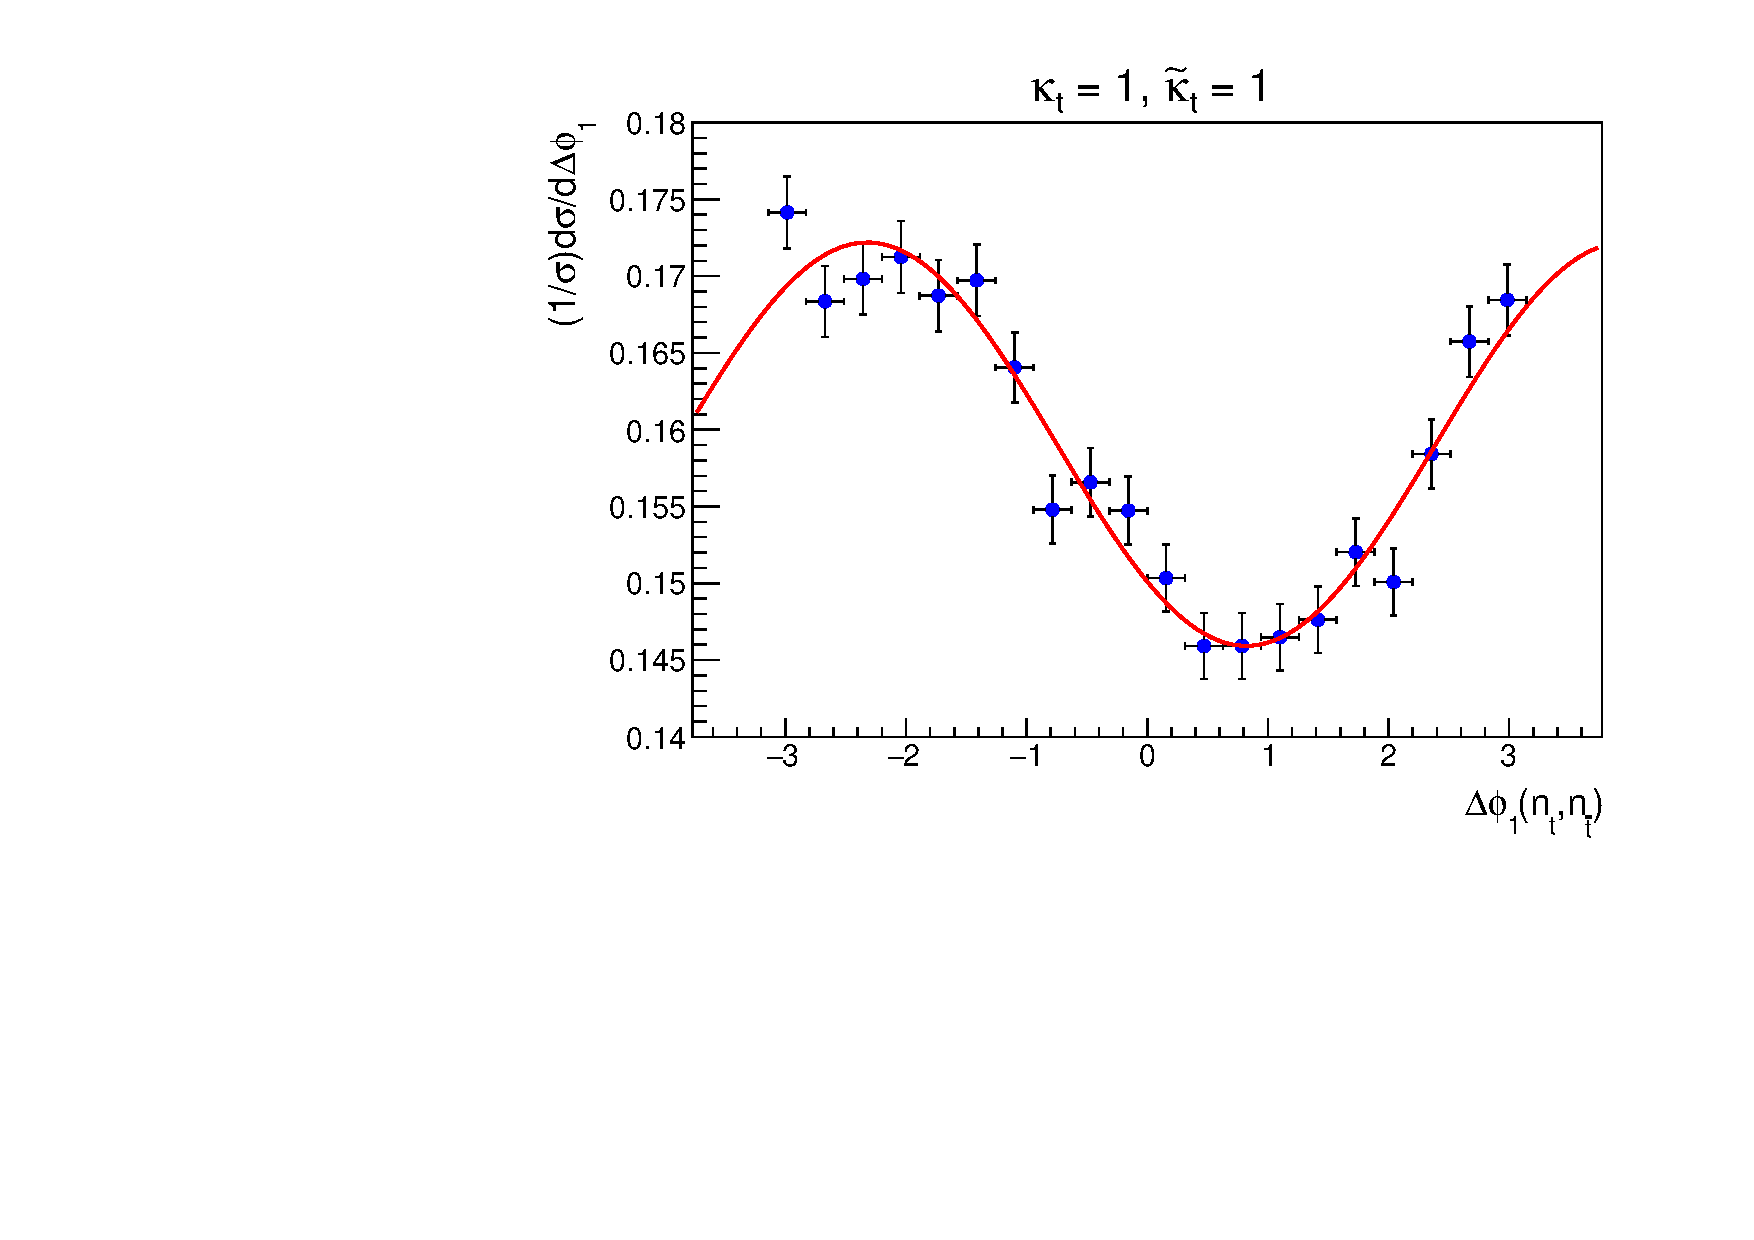
\includegraphics[scale=0.45]{TP1_11_nocuts_nuevo.pdf}}
\hspace*{-0.006\textwidth}
\subfloat{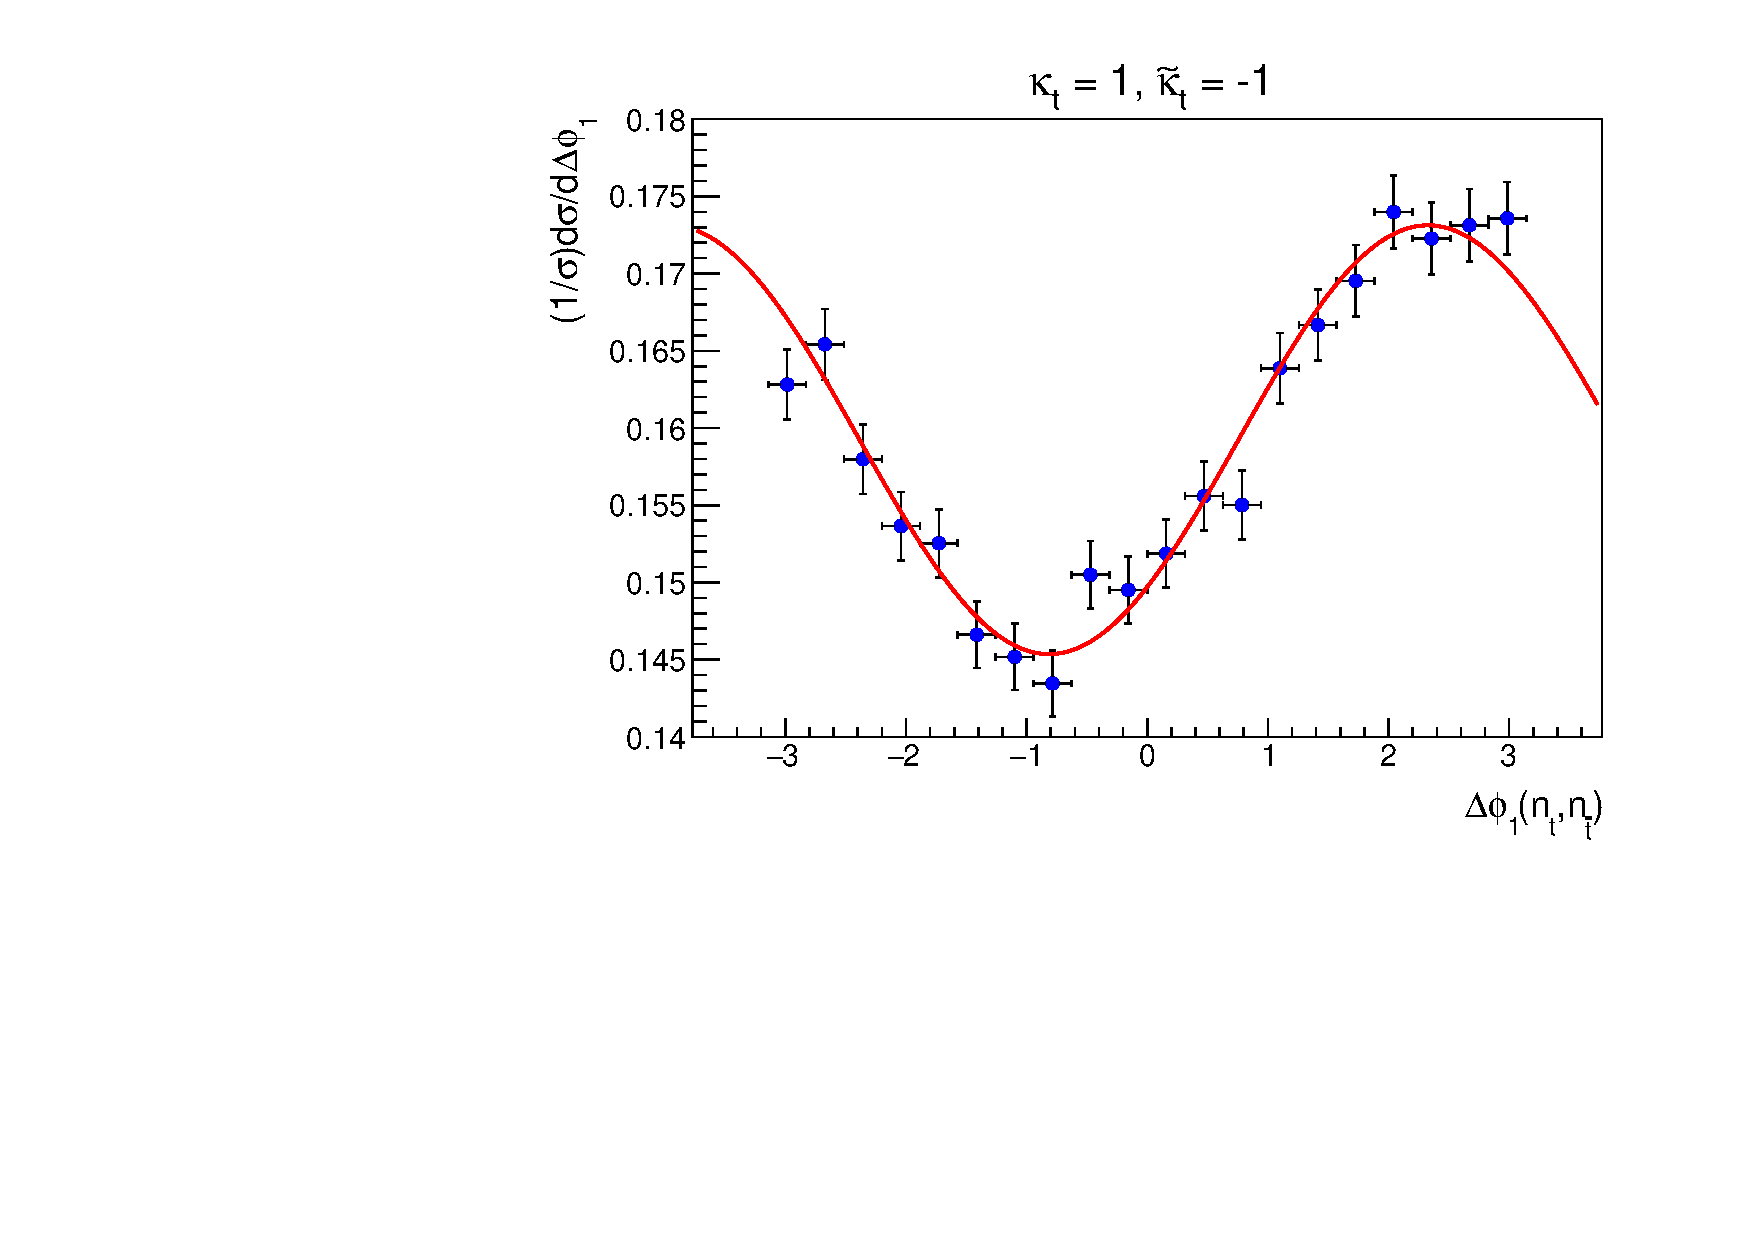
\includegraphics[scale=0.45]{TP1_1-1_nocuts_nuevo.pdf}} \\
\hspace*{-0.52cm}
%\hspace*{0.03\textwidth}
\subfloat{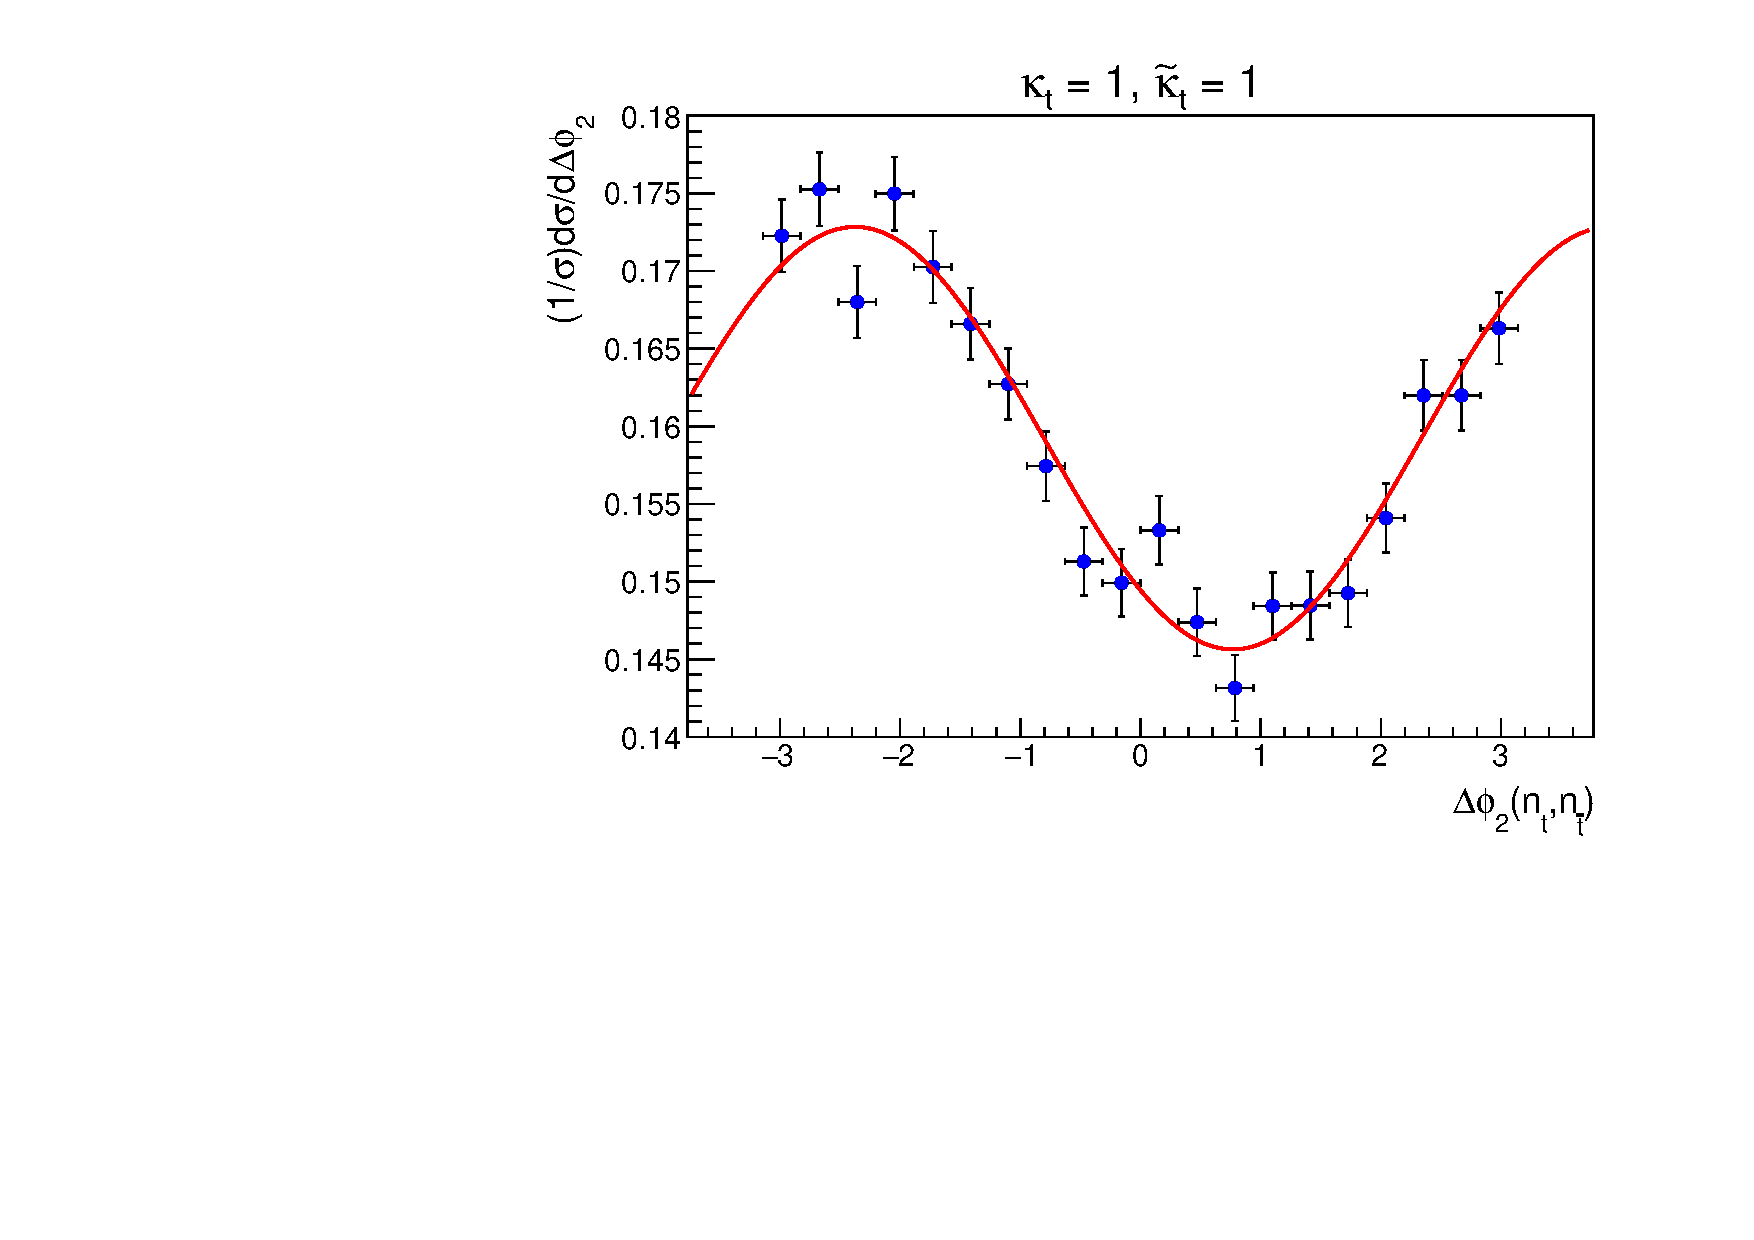
\includegraphics[scale=0.45]{TP2_11_nocuts_nuevo.pdf}}
\hspace*{-0.006\textwidth}
\subfloat{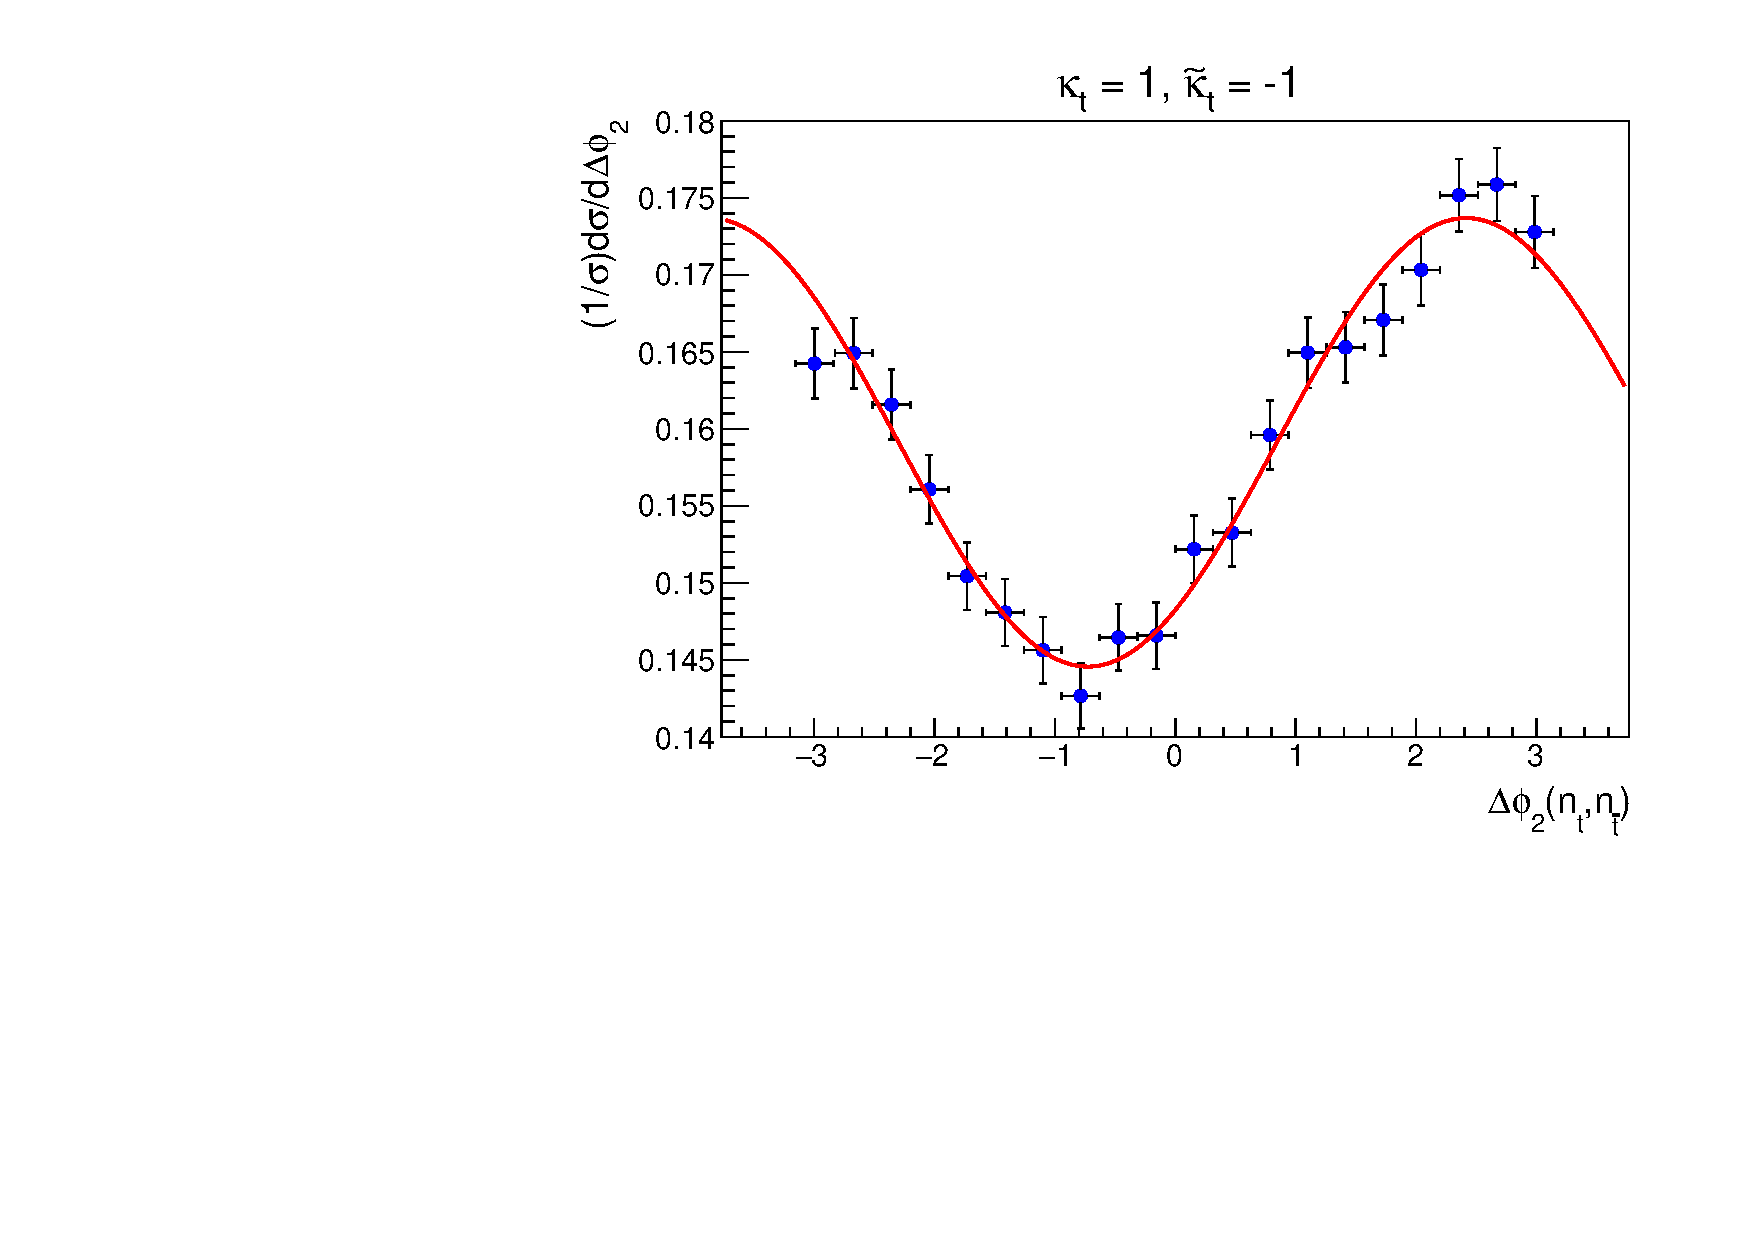
\includegraphics[scale=0.45]{TP2_1-1_nocuts_nuevo.pdf}}
\caption{Angular distributions $d\sigma/(\sigma
  d\Delta\phi_1(n_t,n_{\tbar}))$ (top) and $d\sigma/(\sigma
  d\Delta\phi_2(n_t,n_{\tbar}))$ (bottom) associated with the TPs
  $\epsilon_1=\TPa$ and $\epsilon_2=\TPb$ respectively for the
  $\mathrm{CP}$-mixed cases $\kp=\kpt=1$ (left) and $\kp=-\kpt=1$
  (right) when the $\Delta R_{\ell\ell}$ cut is turned off. Also, the
  corresponding fit curves are displayed in red.}
\label{fig7}
\end{figure}
\end{center}
\par Concerning the angular distributions that can be related to the
combination $\epsilon_4$, we have analized the
$\Delta\phi(n_t,n_{\tbar})$ distribution in the $Q$ rest frame with
$H$ in the $z$-axis for various values of $\kp$ and $\kpt$. We have
found that these distributions are not described by Eq.~(\ref{eq27})
and their range of variation is larger than that of the distributions
displayed in Figs.~\ref{fig5} and \ref{fig6}. Unlike the distributions
related to $\epsilon_1$-$\epsilon_3$, those arising from $\epsilon_4$
exhibit small changes in their shapes for all the considered
hypotheses and for this reason we have not included the corresponding
plots here. However, the larger range of variation of the $\epsilon_4$
distributions leads to higher values for the asymmetry (as can be sees
from Tables \ref{table1} and \ref{table2}) even when the changes in
the respective shapes are smaller than in the case of the
distributions described by Eq.~(\ref{eq27}).  \par
%%%%%%%%%%%%%%%%%%%%%%%%%%%%%%%%%%%%%%%%%%%%%%%%%%%%%%%%%%%%%%%%%%%%%%%%%%
\subsection{Mean value}
\label{sec3.3}
We turn now to consider the last type of observables constructed from
the TPs that are sensitive to $\kpt$, the mean value. Given a certain
TP, we define its mean value in the following manner,
%
\beq
\label{eq28}
\langle \epsilon \rangle = \frac{\int\epsilon\, \{d\sigma (pp\to b\,\ell^+\nu_{\ell}\,\bbar\,\ell^-\bar{\nu}_{\ell}H)/ d\Phi\}\,d\Phi}{\int \{d\sigma (pp\to b\,\ell^+\nu_{\ell}\,\bbar\,\ell^-\bar{\nu}_{\ell}H)/ d\Phi\}\,d\Phi},
\eeq
%
where $\Phi$ is the Lorentz invariant phase space corresponding to the
final state
$b\,\ell^+\nu_{\ell}\,\bbar\,\ell^-\bar{\nu}_{\ell}H$. From
Eq.~(\ref{eq20}) we see that only the terms linear in $\kp$ and $\kpt$
will contribute to the mean value, so that we expect this observable
to be sensitive not only to the value but also to the relative sign of
the couplings.\par The results obtained for the TPs $\epsilon_1=
\epsilon(t,\tbar,n_t,n_{\tbar})$, $\epsilon_2=
\epsilon(Q,\tbar,n_t,n_{\tbar})$ and $\epsilon_3
=\epsilon(Q,t,n_t,n_{\tbar})$ introduced in Sec.~\ref{sec2} are
displayed in Table \ref{table5}, where we list the deviation of the
mean values from the SM case ($\kpt = 0$) in terms of the
corresponding statistical uncertainty of the estimator of $\langle
\epsilon \rangle$, $\bar{\epsilon}$.
\renewcommand{\arraystretch}{1.6}
\begin{table}[H]
\caption{Mean values obtained for the TPs $\epsilon_{1,2,3}$ for the
  SM case and two $\mathrm{CP}$-mixed cases with opposite sign in the
  pseudoscalar coupling. The values are obtained by using $10^5$
  simulated events.}
\label{table5}
\begin{center}
\begin{tabular}{|C{1cm}|C{1cm}||C{2cm}||C{2cm}||C{2cm}|}
%\hhline{|=====|}
\hhline{|-----|}
$\kappa_t$ & $\tilde{\kappa}_t$ & $\langle \epsilon_1 \rangle /\sigma_{\bar{\epsilon}_1}$ & $\langle \epsilon_2 \rangle /\sigma_{\bar{\epsilon}_2}$ & $\langle \epsilon_3 \rangle /\sigma_{\bar{\epsilon}_3}$ \\ 
\hhline{|=====|} 
%\hhline{|-----|}
%\vspace*{.5mm}
\renewcommand{\arraystretch}{1.0}
$1$~ & $-1$~~~ & $4.26$~ & $4.94$~ & $-5.81$~~~\\[0.6mm]
\hline
$1$ & $0$~ & $-0.91$~~~ & $-0.22$~~~ & $1.25$~\\[0.6mm]
\hline
$1$ & $1$~ & $-7.98$~~~ & $-8.83$~~~& $8.75$~\\[0.6mm]
\hhline{|=====|}
%\hhline{|-----|}
\end{tabular}
\end{center} 
\end{table}
We see that the three observables are capable of disinguishing the SM
case from both $\mathrm{CP}$-mixed cases. Further, the observables are
sensitive to the sign of $\kpt$ and the two $\mathrm{CP}$-mixed cases
are also clearly disentangled. The observables $\langle \epsilon_2
\rangle$ and $\langle \epsilon_3 \rangle$ appear to be slightly more
sensitive than $\langle \epsilon_1 \rangle$. On the other hand, the
mean value for the combination $\epsilon_4$ introduced in
Sec.~\ref{sec3.1} gives slightly smaller values than those listed in
Table \ref{table5}, with $-4.32, 1.11$ and $7.23$ for the cases
$(\kp=1,\kpt=-1,0,1)$ respectively. As with the asymmetry, the
hypotheses $\mathrm{CP}$-even and $\mathrm{CP}$-odd cannot be
distinguished by the mean value that is also linear in both $\kp$ and
$\kpt$ (see Eqs.~(\ref{eq20}) and (\ref{eq28})). By taking into
account the results given in Sec.~\ref{sec3.1}, we can conclude that
the sensitivity to the NP contribution is smaller for the mean values
than for the asymmetries of the TPs under consideration.
%%%%%%%%%%%%%%%%%%%%%%%%%%%%%%%%%%%%%%%%%%%%%%%%% 
\section{{\boldmath $\mathrm{CP}$}-odd observables not depending on \MakeLowercase{{\boldmath $t$}} and \MakeLowercase{{\boldmath $\tbar$}} spin vectors}
\label{sec4}
So far we have considered three TPs involving the momenta $t,\tbar$
and $Q$ and the spin vectors $n_t$ and $n_{\tbar}$ given in
Eqs.~(\ref{eq3})-(\ref{eq4}). In fact, we have described the general
form of the differential cross-section in terms of these vectors in
Eq.~(\ref{eq20}). Here, we will take into account another
possibilities for the choice of the vectors from which the
$\mathrm{CP}$-odd observables can be constructed. From the definitions
in Eqs.~(\ref{eq3})-(\ref{eq4}), we see that the TPs
$\epsilon_{1,2,3}$ can be written as follows,
%
\beq
\label{eq29}
\TPa = \frac{m^2_t}{(t\cdot \ell^+)(\tbar\cdot \ell^-)}\,\epsilon(t,\tbar,\ell^-\!,\ell^+),
\eeq
%
\vspace*{1mm}
\beq
\label{eq30}
\TPb = \frac{m^2_t}{(t\cdot \ell^+)(\tbar\cdot \ell^-)}\left(\epsilon(t,\tbar,\ell^-\!,\ell^+)+\epsilon(H,\tbar,\ell^-\!,\ell^+)+\frac{(t\cdot\ell^+)}{m^2_t}\epsilon(H,\tbar,t,\ell^-\!)\right)
\eeq
%
\vspace*{1mm}
\beq
\label{eq31}
\TPc = \frac{m^2_t}{(t\cdot \ell^+)(\tbar\cdot \ell^-)}\left(-\epsilon(t,\tbar,\ell^-\!,\ell^+)+\epsilon(H,t,\ell^-\!,\ell^+)+\frac{(\tbar\cdot\ell^-)}{m^2_t}\epsilon(H,\tbar,t,\ell^+\!)\right).
\vspace*{2mm}
\eeq
%
The above equations express the TPs studied in the last sections as
linear combination of TPs involving the momenta $t,\tbar,H,\ell^+$ and
$\ell^-$, with coefficients that are functions of phase space
variables. These five momenta give rise to five TPs whose sensitivity
can also be tested by means of the observables introduced in
Secs.~\ref{sec3.1}-\ref{sec3.3}. In the first place, we have found
that TPs not including both lepton and anti-lepton momenta present a
negligible sensitivity, and then we will concentrate here on the
results obtained for the remaining TPs,
$\epsilon_5\equiv\epsilon(t,\tbar,\ell^-\!,\ell^+),
\epsilon_6\equiv\epsilon(H,t,\ell^-\!,\ell^+)$ and $\epsilon_7\equiv
\epsilon(H,\tbar,\ell^-\!,\ell^+)$. The Tables \ref{table6} and
\ref{table7} summarize the results for these TPs.
\renewcommand{\arraystretch}{1.6}
\begin{table}[H]
\caption{Mean values obtained for the TPs $\epsilon_{5,6,7}$ for the
  SM case and two $\mathrm{CP}$-mixed cases with opposite sign in the
  pseudoscalar coupling. The values correspond to $10^5$ simulated
  events.}
\label{table6}
\begin{center}
\begin{tabular}{|C{1cm}|C{1cm}||C{2cm}||C{2cm}||C{2cm}|}
%\hhline{|=====|}
\hhline{|-----|}
$\kappa_t$ & $\tilde{\kappa}_t$ & $\langle \epsilon_5 \rangle /\sigma_{\bar{\epsilon}_5}$ & $\langle \epsilon_6 \rangle /\sigma_{\bar{\epsilon}_6}$ & $\langle \epsilon_7 \rangle /\sigma_{\bar{\epsilon}_7}$ \\ 
\hhline{|=====|} 
%\hhline{|-----|}
%\vspace*{.5mm}
\renewcommand{\arraystretch}{1.0}
$1$~ & $-1$~~~ & $3.98$~ & $-1.96$~~~ & $1.69$~ \\[0.6mm]
\hline
$1$ & $0$~ & $-0.43$~~~ & $1.25$~ & $0.74$~ \\[0.6mm]
\hline
$1$ & $1$~ & $-6.76$~~~ & $3.46$~ & $-3.29$~~~~\\[0.6mm]
\hhline{|=====|}
%\hhline{|-----|}
\end{tabular}
\end{center} 
\end{table}
\renewcommand{\arraystretch}{1.4}
\begin{table}[H]
\caption{Asymmetries for the TPs $\epsilon_{5,6,7}$ for the SM case
  and the two $\mathrm{CP}$-mixed cases defined by $\kp=1,\kpt=\pm
  1$. The values correspond to $10^5$ simulated events.}
\label{table7}
\begin{center}
\begin{tabular}{|C{1cm}|C{1cm}||C{2cm}|C{2cm}||C{2cm}|C{2cm}||C{2cm}|C{2cm}|}
%\begin{tabular}{|c|r||r|c||r|c||r|c|}
\hhline{|========|}
%\hhline{|--------|}
$\kappa_t$&$\tilde{\kappa}_t$~~&$\mathcal{A}(\epsilon_5)$~~&$\mathcal{A}(\epsilon_5)/\sigma_{\mathcal{A}}$& $\mathcal{A}(\epsilon_6)$~~&$\mathcal{A}(\epsilon_6)/\sigma_{\mathcal{A}}$&$\mathcal{A}(\epsilon_7)$~~&$\mathcal{A}(\epsilon_7)/\sigma_{\mathcal{A}}$  \\ 
\hhline{|========|} 
%\hhline{|--------|}
$1$ & $-1$~~~ & $0.0315$~ & $10.0$~ & $-0.0134$~~~ & $-4.2$~~~ & $0.0111$~ & $3.5$~\\[0.6mm]
\hline
$1$ & $0$ & $-0.0021$~~~ & $-0.7$~~~ & $-0.0011$~~~ & $-0.3$~~~ & $0.0009$~& $0.3$~\\[0.6mm]
\hline
$1$ & $1$ & $-0.0379$~~~ & $-12.0$~~~ & $0.0143$~ & $4.5$~ & $-0.0137$~~~ & $\,-4.3$~~~  \\[0.6mm]
\hhline{|========|}
%\hhline{|--------|}
\end{tabular}
\end{center} 
\end{table}
\par
%
We see that the TP $\epsilon_5$ gives rise to asymmetries and mean
values that are clearly higher than those obtained from $\epsilon_6$
and $\epsilon_7$. This is in contrast to the TPs $\epsilon_{1,2,3}$,
for which the asymmetries and mean values are comparable (see Tables
\ref{table1} and \ref{table5}). We also note that the asymmetry for
$\epsilon_5$ is exactly the same as for $\epsilon_1$ as was expected
from Eq.~(\ref{eq29}) since the proportionality factor relating them
is positive definite. Regarding the mean values, we see by comparing
Tables \ref{table5} and \ref{table6} that the TPs $\epsilon_{1,2,3}$
appear to have a higher sensitivity to the pseudoscalar coupling than
$\epsilon_{5,6,7}$.  \par It is important to mention that in the
$t\tbar$ rest frame the sign of the TP $\epsilon_5$ is defined through
the angle $\Delta\phi_{\ell^-\ell^+}$ (recall the discussion on
Eq.~(\ref{eq28})), which is the angular difference between the
projections of the leptons momenta onto the plane perpendicular to
$\vec{\tbar}$. By a similar argument to that discussed at the
beginning of Sec.~\ref{sec3.2}, we can construct an associated angular
distribution that, being constrained by the $\mathcal{A}(\epsilon_5)$,
will be also sensitive to the sign of the pseudoscalar coupling. This
angular variable is nothing but that proposed in \cite{Ellis} as a
useful $\mathrm{CP}$-odd observable. Moreover, it is shown in
\cite{Ellis} that this angular distribution follows the functional
form given in Eq.~(\ref{eq27}). Due to the fact that this distribution
is constrained by $\mathcal{A}(\epsilon_5)$ which is equal to
$\mathcal{A}(\epsilon_1)$ and smaller than
$\mathcal{A}(\epsilon_{2,3})$, the corresponding shifts ($\delta$)
obtained for different values of $\kpt$ are expected to be of the same
order than those exhibited by the $\Delta\phi_1(n_t,n_{\tbar})$
distribution and somewhat smaller than those observed in the
$\Delta\phi_2(n_t,n_{\tbar})$ distribution.  \par In analogy to the
combination of TPs considered in Sec.~\ref{sec3}, we have found a
combination of the TPs $\epsilon_{5,6,7}$ for which the asymmetry is
enhanced with respect to $\epsilon_5$-$\epsilon_7$,
%
\beq
\label{eq32}
\epsilon_8 = 2\epsilon_5 -\epsilon_6 +\epsilon_7 = \epsilon(t+\tbar+H,t-\tbar,\ell^+,\ell^-).
%2\epsilon(t,\tbar,\ell^-,\ell^+)+\epsilon(H,\tbar,\ell^-,\ell^+)-\epsilon(H,t,\ell^-,\ell^+)
\eeq
%
We see from Eq.~(\ref{eq32}) that in the $t\tbar H$ rest frame
$\epsilon_8=M_{t\tbar H}(\vec{t}-\vec{\tbar})\cdot (\vec{\ell}^+\!
\times \vec{\ell}^-)$, where $M_{t\tbar H}$ is the invariant mass of
the system $t\tbar H$. Hence, in this reference frame the sign of the
combination $\epsilon_8$ is set by the quantity
$(\vec{t}-\vec{\tbar})\cdot (\vec{\ell}^+\! \times
\vec{\ell}^-)$. Taking into account Eqs.~(\ref{eq24}) and (\ref{eq32})
along with the definition $Q=(t+\tbar+H)/2$, we see that the only
relevant difference between $\epsilon_4$ and $\epsilon_8$ is that in
the latter the spin vectors $n_t$ and $n_{\tbar}$ have been replaced
by the momenta of the leptons $\ell^+$ and $\ell^-$ respectively. The
values obtained for $\mathcal{A}(\epsilon_8)$ are shown in Table
\ref{table8}. Compared to the TPs $\epsilon_5$-$\epsilon_7$ and
$\epsilon_1, \epsilon_3$ (see Tables \ref{table1} and \ref{table7}),
the chosen combination exhibits a slightly higher sensitivity in the
asymmetry for resolving the $\mathrm{CP}$-mixed cases. This is not
true in the case of the TPs $\epsilon_2$ and $\epsilon_4$, for which
the asymmetry is larger (see Tables \ref{table1}, \ref{table2} and
\ref{table8}). In particular, the comparison between $\epsilon_4$ and
$\epsilon_8$ indicates that the use of the momenta of the leptons
instead of the spin vectors produces a decrease in the sensitivity of
the asymmetry. \par From the TPs $\epsilon_5$-$\epsilon_7$ one can
derive various angular distributions in the same manner we have
discussed in Sec.~\ref{sec3.2} for $\epsilon_1$-$\epsilon_3$. Of
course, in this case the corresponding angle will be defined in terms
of the momenta of the leptons instead of using the spin vectors. These
distributions have the same behaviour than those derived from
$\epsilon_1$-$\epsilon_3$, but only the shift obtained in the case of
$\epsilon_5$ is compatible to the values given in Tables for
$\epsilon_1$-$\epsilon_3$. The shifts resulting from the fit of the
distributions related to $\epsilon_6$ and $\epsilon_7$ are
smaller. Taking into account these facts we do not give further
details of the angular distributions for the TPs discussed in this
section.\par The mean value of $\epsilon_8$ for the hypotheses under
consideration is comparable with the values listed in Table
\ref{table6} for $\epsilon_5$. Concerning the associated angular
distributions, their range of variation is larger than in the case of
the distributions related to $\epsilon_5$-$\epsilon_7$ but exhibit
smaller changes in their shapes for the different hypothesis and for
this reason we do not include here the corresponding plots.
\begin{table}[H]
\caption{Asymmetry for the TP $\epsilon_{8}$ for the SM case and the
  two $\mathrm{CP}$-mixed cases defined by $\kp=1,\kpt=\pm 1$. The
  values are obtained with $10^5$ simulated events.}
\label{table8}
\begin{center}
\begin{tabular}{|C{1cm}|C{1cm}||C{2cm}|C{2cm}|}
%\begin{tabular}{|c|r||r|c||r|c||r|c|}
\hhline{|====|}
%\hhline{|--------|}
$\kappa_t$&$\tilde{\kappa}_t$~~&$\mathcal{A}(\epsilon_8)$~~&$\mathcal{A}(\epsilon_8)/\sigma_{\mathcal{A}}$ \\ 
\hhline{|====|} 
%\hhline{|--------|}
$1$ & $-1$~~~ & $0.0331$~ & $10.5$~ \\[0.6mm]
\hline
$1$ & $0$ & $0.0023$~ & $0.7$~ \\[0.6mm]
\hline
$1$ & $1$ & $-0.0403$~~~ & $\,-12.7$~~~~ \\[0.6mm]
\hhline{|====|}
%\hhline{|--------|}
\end{tabular}
\end{center} 
\end{table}
\section{{\boldmath{$\mathrm{CP}$}}-odd observables not depending on \MakeLowercase{{\boldmath $t$}} and \MakeLowercase{{\boldmath $\tbar$}} momenta}
\label{sec5}
All the observables discussed in the above sections involve the
momenta of the top and anti-top quarks thus requiring the full
reconstruction of the kinematics of the individual $t$ and $\tbar$
systems in order to be measured. Although challenging due to the
presence of two neutrinos in the final state, this can be in principle
done by applying a kinematic reconstruction method such that the
neutrino weighting technique \cite{atlasconf,atlascharge}. Another
possibility is to define observables that are not dependent on the $t$
and $\tbar$ momenta but make use of the quarks $b$ and $\bbar$. In
order to construct such observables we will modify here the most
sensitive observables studied in Secs.~\ref{table3} and \ref{sec4},
namely the combinations $\epsilon_4$ and $\epsilon_8$
respectively. Let us first consider the combination $\epsilon_8$
defined in Eq.~(\ref{eq32}) and replace the top and antitop momenta by
the bottom and antibottom momenta respectively. Thus, we define
%
\beq
\label{eq33}
\epsilon_9 = \epsilon(b+\bbar+H,b-\bbar,\ell^+,\ell^-).
\eeq
%
Note that now the sign of the TP $\epsilon_9$ is set by the sign of
the quantity $(\vec{b}-\vec{\bbar})\cdot(\vec{\ell}^+\!\times
\vec{\ell}^-)$ in the $b\bbar H$ rest frame. This quantity is in fact
used in \cite{Guadagnoli} but in the lab frame in order to define a
$\mathrm{CP}$-odd observable that only depends on lab frame
variables. The values of the asymmetry for $\epsilon_9$ are listed in
Table \ref{table9}. By comparing Tables \ref{table8} and \ref{table9}
we see that the use of the $b,\bbar$ instead of $t,\tbar$ leads to a
decrese in the sensitivity of the asymmetry by $\sim 5\sigma$ for
$\kp=1,\kpt=\pm 1$. However, the observable is still capable of
discriminating not only between the two $\mathrm{CP}$-mixed hypotheses
but also between these and the SM case.
%\newpage
We proceed now in a similar way with the combination $\epsilon_4$. By
using Eq.~(\ref{eq24}) along with the definitions of the spin vectors
in Eqs.~(\ref{eq3})-(\ref{eq4}), we can write
%
\beq
\label{eq34}
\epsilon_4 = \frac{m^2_t}{(t\cdot\ell^+)\cdot(\tbar\cdot\ell^-)}\,\epsilon(Q,t-\tbar,\ell^-,\ell^+)+\frac{1}{(t\cdot\ell^+)}\,\epsilon(Q,t,\ell^+,\tbar)-\frac{1}{(\tbar\cdot \ell^-)}\,\epsilon(Q,\tbar,t,\ell^-).
\eeq
%
Since the asymmetry is not changed by an overall positive definite
factor, we will concentrate on the following combination arising from
the expression in Eq.~(\ref{eq34}),
%
\beq
\label{eq35}
\epsilon(Q,t-\tbar,\ell^-,\ell^+)+\frac{(\tbar\cdot \ell^-)}{m^2_t}\epsilon(Q,t,\ell^+,\tbar)-\frac{(t\cdot\ell^+)}{m^2_t}\epsilon(Q,\tbar,t,\ell^-),
\eeq
%
\begin{table}[H]
\caption{Asymmetry for the TP $\epsilon_{9}$ for the SM case and the
  two $\mathrm{CP}$-mixed cases defined by $\kp=1,\kpt=\pm 1$. The
  values are obtained with $10^5$ simulated events.}
\label{table9}
\begin{center}
\begin{tabular}{|C{1cm}|C{1cm}||C{2cm}|C{2cm}|}
%\begin{tabular}{|c|r||r|c||r|c||r|c|}
\hhline{|====|}
%\hhline{|--------|}
$\kappa_t$&$\tilde{\kappa}_t$~~&$\mathcal{A}(\epsilon_9)$~~&$\mathcal{A}(\epsilon_9)/\sigma_{\mathcal{A}}$ \\ 
\hhline{|====|} 
%\hhline{|--------|}
$1$ & $-1$~~~ & $0.0171$~ & $5.4$~ \\[0.6mm]
\hline
$1$ & $0$ & $0.0010$~ & $0.3$~ \\[0.6mm]
\hline
$1$ & $1$ & $-0.0247$~~~ & $\,-7.8$~~~~ \\[0.6mm]
\hhline{|====|}
%\hhline{|--------|}
\end{tabular}
\end{center} 
\end{table}
\noindent
%
and instead of replacing $t$ and $\tbar$ directly by $b$ and $\bbar$,
we use their visible parts, namely $b+\ell^+$ and $\bbar +\ell^-$
respectively. This results in the following definition
%
\beq
\label{eq36}
\epsilon_{10}=\epsilon(\tilde{Q},c_{b\bbar}\,,\ell^-,\ell^+)-w_1\,\epsilon(\tilde{Q},b,\bbar,\ell^+)+w_2\,\epsilon(\tilde{Q},b,\bbar,\ell^-),
\eeq
%
where $\tilde{Q}\equiv (b+\ell^+\!+\bbar +\ell^-)/2$ stands for the
visible part of $Q$, $c_{b\bbar}=(1-w_1)\,b-(1-w_2)\,\bbar$ and the
weights $w_{1,2}$ are given by $(\bbar\cdot \ell^-)/m^2_t $ and
$(b\cdot \ell^+)/m^2_t$ respectively. Also, the contribution
$m^2_{\ell}/m^2_t$ has been neglected both in $w_1$ and in $w_2$. Note
that if we set $w_1=w_2=0$, the combination $\epsilon_{10}$ reduces to
$\epsilon_9 /2$ and $\mathcal{A}(\epsilon_{10})$ becomes equal to
$\mathcal{A}(\epsilon_9)$. The results obatined for the asymmetry of
$\epsilon_{10}$ are given in Table \ref{table10}. By comparing Tables
\ref{table2} and \ref{table10} we see again that the sensitivity of
the asymmetry decreases when $t$ and $\tbar$ are not included in the
TP. Nevertheless, the combination $\epsilon_{10}$ remains a useful
observable for discriminating the $\mathrm{CP}$ nature of the Higgs
boson, with the corresponding asymmetry having a sensitivity even
higher than that of $\epsilon_9$, as can be checked by taking into
account Tables \ref{table9} and \ref{table10}. More precisely, the
separation between the $\mathrm{CP}$-mixed hypotheses is enhanced by
about $3\sigma$. This improvement in the asymmetry of $\epsilon_{10}$
with respect to $\epsilon_9$ may be due to two facts. In the first
place, as was pointed out in Sec.~\ref{sec4} when comparing the TPs
$\epsilon_4$ and $\epsilon_8$, the asymmetry appears to be higher when
the spin vectors are used instead of the lepton momenta and we see
from Eqs.~(\ref{eq33}) and (\ref{eq36}) that $\epsilon_{10}$, being
obtained from $\epsilon_4$, contains the information on the spin
vectors, as opposed to $\epsilon_9$ that depends directly on the
lepton momenta because it is derived from $\epsilon_8$. In the second
place, in order to obtain $\epsilon_{10}$ we have replaced in the
expression for $\epsilon_4$ the top and antitop momenta by their
visible part, while in the case of $\epsilon_9$ the bottom and
antibottom momenta have been used.
\begin{table}[H]
\caption{Asymmetry for the TP $\epsilon_{10}$ for the SM case and the
  two $\mathrm{CP}$-mixed cases defined by $\kp=1,\kpt=\pm 1$. The
  values are obtained by using $10^5$ simulated events.}
\label{table10}
\begin{center}
\begin{tabular}{|C{1cm}|C{1cm}||C{2cm}|C{2cm}|}
%\begin{tabular}{|c|r||r|c||r|c||r|c|}
\hhline{|====|}
%\hhline{|--------|}
$\kappa_t$&$\tilde{\kappa}_t$~~&$\mathcal{A}(\epsilon_{10})$~~&$\mathcal{A}(\epsilon_{10})/\sigma_{\mathcal{A}}$ \\ 
\hhline{|====|} 
%\hhline{|--------|}
$1$ & $-1$~~~ & $-0.0213$~~~ & $-6.7$~~~ \\[0.6mm]
\hline
$1$ & $0$ & $0.0031$~ & $1.0$~ \\[0.6mm]
\hline
$1$ & $1$ & $0.0300$~ & $9.5$~ \\[0.6mm]
\hhline{|====|}
%\hhline{|--------|}
\end{tabular}
\end{center} 
\end{table}
\par
%
By using our set of simulated events we have also tested, for
comparison purposes, the asymmetry of the lab frame observable given
in \cite{Guadagnoli}. We have obtained that this observable appears to
be slightly less sensitive than the combination $\epsilon_{10}$,
giving rise to a separation between the $\mathrm{CP}$-mixed hypotheses
smaller by about $1.4\sigma$.
\section{Experimental Feasibility}
\label{sec6}
%
By considering the mild selection cuts introduced in Sec.~\ref{sec3},
the SM cross section for $\ppprocess$, $\ell=e,\mu$ at
$14\,\mathrm{TeV}$ is $\sim 15.3\,\mathrm{fb}$ and hence the number of
events expected within the context of the HL-LHC is $\sim
15.3\,\mathrm{fb} \times 3000\,\mathrm{fb}^{-1} = 4.59\times
10^4$. This number is expected to be even larger in the case of
$\kp=1,\kpt\neq 0$ since the corresponding cross section is then
higher than the SM one. By taking into account NLO corrections to the
production process and considering a $K$-factor around $1.2$
\cite{Dawson,Beenakker,Dittmaier}, the number of events can be raised
up to $\sim 5.49 \times 10^4$. On the other hand, additional cuts as
well as the efficiency related to the reconstruction of particles
momenta will contribute to decrease this number. For instance, in
order to obtain the asymmetry of $\epsilon_4$, the $t$ and $\tbar$
momenta need to be reconstructed. This is challenging not only due to
the presence of two neutrinos in the final state which escape the
detector undetected but also because final state objects need to be
asocciated with the respective parent quark \cite{atlasconf}. As was
already mentioned in Sec.~\ref{sec5}, a possibility is to use the
neutrino weighting technique along with the kinematic equations
arising from kinematic constraints related to the top and $W$ masses
as well as from the energy-momentum conservation at each of the decay
vertices involved in the process. Within the context of $t\tbar$ this
procedure has been used, for instance, in order to obtain measurements
of spin correlation \cite{atlasconf} and charge asymmetry
\cite{atlascharge}. Also, events reconstructed with this technique has
been used in \cite{dosSantos} for analyzing angular distributions that
are useful for discriminating the signal from the backgrounds in
$t\tbar H (H\rightarrow b\bbar)$. In all these cases the corresponding
efficiency in the reconstruction of the momenta is up to $\sim 80
\%$.\par Based on the discussion given in the previous paragraph, we
have simulated sets of $5\times 10^4, 1\times 10^4$ and $5\times 10^3$
events and recalculated the most sensitive observable, namely
$\mathcal{A}(\epsilon_4)$, for each case. The results are displayed in
Table \ref{table11}, where it can be seen that for a number of events
close to that roughly estimated above within the context of the
HL-LHC, the observable is still sensitive to $\kpt$ allowing to
separate the $\mathrm{CP}$-mixed cases by $19\sigma$. As expected, the
sensitivity worsen as the number of events is reduced, but even with
$5\times 10^3$ events the separation between the $\mathrm{CP}$-mixed
hypotheses under consideration is around $6.5\sigma$. \par Although
the combination $\epsilon_{10}$ discussed in Sec.~\ref{sec5} avoids
the problem of reconstructing the top and antitop momenta, we have
also considered the respective asymmetry obtained for more
conservative numbers of events. In Table \ref{table12} we show the
results for $\mathcal{A}(\epsilon_{10})$ when the number of events is
reduced from $5\times 10^4$ to $1\times 10^4$. We see in this case
that even with $1\times 10^4$ simulated events the observable is
capable to discriminate the $\mathrm{CP}$-mixed cases by
$5.6\sigma$.\par Finally, it is important to mention that a realistic
analysis of the sensistivity of the observables discussed in this
paper requires the study of the impact of the backgrounds as well as
the hadronization of the quarks in the final state and the effects of
the detector. If we consider the dominant decay mode of the higgs,
$H\rightarrow b\bbar$, in order to maximize the cross section of the
process, the signature is given by $4$ $b$-jets, two leptons and
missing energy, while the main background arise from the production of
$t\tbar$ in asocciation with additional jets, being the dominant
source the production of $t\tbar + b\bbar$. By applying a small set of
cuts it is shown in \cite{chinos} that the
\begin{table}[H]
\caption{Asymmetry for the TP $\epsilon_4$ obtained by using $5\times
  10^4, 1 \times 10^4$ and $5\times 10^3$ simulated events for the SM
  case and the two $\mathrm{CP}$-mixed cases defined by
  $\kp=1,\kpt=\pm 1$. }
\label{table11}
\begin{center}
\begin{tabular}{|C{1cm}|C{1cm}||C{2cm}|C{2cm}||C{2cm}|C{2cm}||C{2cm}|C{2cm}|}
%\begin{tabular}{|c|r||r|c||r|c||r|c|}
\hhline{|========|}
%\hhline{|--------|}
\multirow{2}{*}{$\kappa_t$} & \multirow{2}{*}{$\tilde{\kappa}_t$} & \multicolumn{2}{c||}{$N_{\mathrm{ev}}=5\times 10^4$} & \multicolumn{2}{c||}{$N_{\mathrm{ev}}=1\times 10^4$} & \multicolumn{2}{c|}{$N_{\mathrm{ev}}=5\times 10^3$} \\ \cline{3-8}
& & $\mathcal{A}(\epsilon_4)$~~&$\mathcal{A}(\epsilon_4)/\sigma_{\mathcal{A}}$ &  $\mathcal{A}(\epsilon_4)$~~&$\mathcal{A}(\epsilon_4)/\sigma_{\mathcal{A}}$ &  $\mathcal{A}(\epsilon_4)$~~&$\mathcal{A}(\epsilon_4)/\sigma_{\mathcal{A}}$ \\
\hhline{|========|} 
%\hhline{|--------|}
$1$ & $-1$~~~ & $-0.0405$~~~ & $-9.1$~~~ & $-0.0426$~~~ & $-4.3$~~~ & $-0.0496$~~~ & $-3.5$~~~ \\[0.6mm]
\hline
$1$ & $0$ & $0.0004$~ & $0.1$~ & $-0.0084$~~~ & $-0.8$~~~ & $-0.0004$~~~ & $-0.03$~~~ \\[0.6mm]
\hline
$1$ & $1$ & $0.0443$~ & $9.9$~ & $0.0434$~ & $4.2$~ & $\,0.0420$~ & $3.0\,\,$ \\
\hhline{|========|}
%\hhline{|--------|}
\end{tabular}
\end{center} 
\end{table}
\begin{table}[H]
\caption{Asymmetry for the TP $\epsilon_{10}$ in the SM case and the
  two $\mathrm{CP}$-mixed cases defined by $\kp=1,\kpt=\pm 1$ when the
  number of simulated events is reduced from $5\times 10^4$ to $1
  \times 10^4$.}
\label{table12}
\begin{center}
\begin{tabular}{|C{1cm}|C{1cm}||C{2cm}|C{2cm}||C{2cm}|C{2cm}|}
%\begin{tabular}{|c|r||r|c||r|c||r|c|}
\hhline{|======|}
%\hhline{|--------|}
\multirow{2}{*}{$\kappa_t$} & \multirow{2}{*}{$\tilde{\kappa}_t$} & \multicolumn{2}{c||}{$N_{\mathrm{ev}}=5\times 10^4$} & \multicolumn{2}{c|}{$N_{\mathrm{ev}}=1\times 10^4$} \\ \cline{3-6}
& & $\mathcal{A}(\epsilon_{10})$~~&$\mathcal{A}(\epsilon_{10})/\sigma_{\mathcal{A}}$ &  $\mathcal{A}(\epsilon_{10})$~~&$\mathcal{A}(\epsilon_{10})/\sigma_{\mathcal{A}}$ \\
\hhline{|======|} 
%\hhline{|--------|}
$1$ & $-1$~~~ & $-0.0270$~~~ & $-6.0$~~~ & $-0.0184$~~~ & $-1.8$~~~  \\[0.6mm]
\hline
$1$ & $0$ & $0.0022$~ & $0.5$~ & $-0.0086$~~~ & $-0.9$~~~  \\[0.6mm]
\hline
$1$ & $1$ & $0.0313$~ & $7.0$~ & $0.0380$~ & $3.8\,$ \\
\hhline{|======|}
%\hhline{|--------|}
\end{tabular}
\end{center} 
\end{table}
\noindent
%
signal to background ratio is largely improved. On the other hand, a
rigorous treatment of the backgrounds and their impact with respect to
the signal is performed in \cite{atlasger} by using $20.3\,
\mathrm{fb}^{-1}$ of data at $\sqrt{s}=8\,\mathrm{TeV}$.  \par The
results shown in tables \ref{table11} and \ref{table12} reveal that
with $5\times 10^3$ and $1\times 10^4$ events respectively the
observables $\mathcal{A}(\epsilon_4)$ and $\mathcal{A}(\epsilon_{10})$
are still useful for testing $\kpt$. Without considering the lack of
events related to the experimental analysis, these numbers of events
correspond to a luminosity around $\sim
300\,$-$\,600\,\mathrm{fb}^{-1}$ for the SM and even smaller for the
$\mathrm{CP}$-mixed cases due to the larger cross section. This range
of luminosities is in principle achievable in the short term by the
LHC. We note that in order to be fully conclusive about the required
luminosity, it is important to include the effects of hadronization,
detector resolution, reconstruction eficciencies and so
forth. However, this kind of analysis is out of the scope of this
paper.
%%%%%%%%%%%% with Cuts
%51.46/17 -0.02 +- 0.08
%45.48/17  -1.09 +- 0.07
%65.60/17   0.96 +- 0.08
%28.84/17   0.02 +- 0.07
%%%%%%%
%9.13/17     0.01 +- 0.06
%9.05/17     -0.98 +- 0.07
%19.7/17     0.80 +- 0.07
%16.59/17    0.06 +- 0.07
%
%%%%%%%%%%%% without Cuts
%16.36/17    0.0022 +-0.06
%15.25/17    -0.82 +- 0.07
%12.80/17    0.81 +- 0.07
%19.38/17    0.11 +- 0.08
%%%%%%
%7.45/17    0.005 +- 0.06
%18.17/17   -0.77 +- 0.07
%9.59/17    0.73 +- 0.06
%12.39/17   0.09 +- 0.08
%%%%%%%%%%%%%%%%%%%%%%%%%%%%%%%%%%%%%%%%%%%%%%%%%
\section{Conclusions}
\label{sec7}
%
In this paper we have presented a collection of $\mathrm{CP}$-odd
observables based on triple product correlations that are useful for
disentangling the relative sign between the scalar ($\kp$) and a
potential pseudoscalar ($\kpt$) top-Higgs couplings in the $t\tbar H$
production with both tops decaying leptonically. We have tested the
sensitivity of the proposed observables by considering three types of
observables: asymmetries, mean values and angular distributions.\par

Through the use of spinor techniques we have written the expression
for the differential cross section of the full process in such a
manner that the production and the decay parts are separated, although
connected by the spin vectors of the top and antitop which are given
in terms of the momenta of the leptons in the final state. Moreover,
we have indentified the terms linear in $\kp$ and $\kpt$ as those
involving TPs. Among these, we have explored the three that do not
involve the momenta of the incoming quarks/gluons and at the same time
incorporate both spin vectors: $\epsilon_1\equiv \TPa$,
$\epsilon_2\equiv \TPb$ and $\epsilon_3\equiv \TPc$.\par We have found
that $\epsilon_{1,2,3}$ allow to distinguish between the
$\mathrm{CP}$-mixed hypotheses by more than $\sim 20\sigma$ in the
case of asymmetries and $\sim 10\sigma$ in the case of mean values
when $1 \times 10^5$ simulated events are used. Furthermore, we have
shown that the angular distributions asocciated with these TPs are
also sensitive to the value of $\kp$ and $\kpt$ exhibiting a phase
shift that varies according to the values taken by these couplings. On
the other hand, by exploring TPs that incorporate the momenta of the
Higgs and the leptons instead of the spin vectors we can conclude that
the observables studied here appear to be more sensitive when the spin
vectors are used.\par

On the other hand, we have proposed a combination of the TPs
considered in the first place, $\epsilon_4\equiv
\epsilon_3-\epsilon_2$, that exhibits the highest sensitivity with the
separation between the $\mathrm{CP}$-mixed hypotheses being increased
by at least $3\sigma$ in the asymmetry for $1 \times 10^5$ events with
respect to $\mathcal{A}(\epsilon_{1,2,3})$. Again, when a similar
combination is constructed by using the leptons momenta instead of the
spin vectors ($\epsilon_8$), the sensitivity in the asymmetry is
decreased by $\sim 3\sigma$ compared to $\mathcal{A}(\epsilon_4)$ for
the same number of events, giving values compatible with those
obtained for the asymmetry of $\epsilon_2$ and $\epsilon_3$. \par

Taking into account the challenge of reconstructing the top and
antitop momenta due to the presence of two neutrinos in the final
state, we have proposed and tested two TP correlations that avoid this
difficulty. The first one is obtained by replacing the $t$ and $\tbar$
by the $b$ and $\bbar$ momenta ($\epsilon_9$), whereas the second
includes the visible part of the $t$ and $\tbar$ momenta
($\epsilon_{10}$). We have encountered that the latter is the most
sensitive leading to a discrimination of the $\mathrm{CP}$-mixed cases
under analysis by up to $\sim 16\sigma$.\par

Finally we have discussed the feasibility of the most sensitive
observables proposed here. We have found that with $5\times 10^3$ and
$1\times 10^4$ events respectively the observables
$\mathcal{A}(\epsilon_4)$ and $\mathcal{A}(\epsilon_{10})$ are still
useful for testing the hypotheses $(\kp=1,\kpt=\pm 1)$ giving rise to
separations of order $\sim 6\sigma$. These required number of events
would be reachable in principle in the short term by the LHC and hence
the capability of the observables studied here for testing the sign of
$\kpt/\kp$ could be probed in that context.

%%%%%%%%%%%%%%%%%%%%%%%%%%%%%%%%%%%%%%%%%%%%%%%%%
\bigskip
\noindent
{\bf Acknowledgments}
\noindent 
This work has been partially supported by ANPCyT under grants No. PICT
2013-0433 and No. PICT 2013-2266, and by CONICET (NM, AS). The work of
KK was supported by the U.S.  National Science Foundation under Grant
PHY-1215785. KK also acknowledges sabbatical support from Taylor
University.
%%%%%%%%%%%%%%%%%%%%%%%%%%%%%%%%%%%%%%%%%%%%%%%%%
\section*{\refname}
\let\bibsection\relax

\setlength{\bibsep}{10pt}
\bibliography{PaperDraftbiblio}
\bibliographystyle{apsrev4-1}

\end{document}
